\documentclass[11pt,a4paper]{article}
% ---- 页面与字体 ----
\usepackage[margin=1in]{geometry}
\usepackage{microtype}
\usepackage{lmodern}
\usepackage[T1]{fontenc}
\usepackage[utf8]{inputenc}
% ---- 数学与算法 ----
\usepackage{amsmath, amssymb, amsfonts, amsthm}
\usepackage{bm}
\usepackage{mathtools}
\usepackage{algorithm}
\usepackage{algorithmic}
% ---- 图表 ----
\usepackage{graphicx}
\usepackage{placeins}
\graphicspath{{figures/}}

\usepackage{booktabs}
\usepackage{xcolor}
\usepackage{enumitem}
\usepackage{caption}
\usepackage{subcaption}
% ---- 引用与超链接 ----
\usepackage[numbers,sort&compress]{natbib}
\usepackage{hyperref}
\hypersetup{
    colorlinks=true,
    linkcolor=blue!50!black,
    citecolor=blue!50!black,
    urlcolor=blue!50!black
}
\usepackage{url}
% ---- 作者信息排版（arXiv 风格） ----
\usepackage{authblk}
% ---- 自定义命令 ----
\newcommand{\R}{\mathbb{R}}
\newcommand{\xopt}{x_*}
\newcommand{\Deltak}{\Delta_k}
\newcommand{\norm}[1]{\left\| #1 \right\|}
\DeclareMathOperator*{\argmin}{arg\,min}
% ---- 定理环境 ----
\newtheorem{theorem}{Theorem}[section]
\newtheorem{lemma}[theorem]{Lemma}
\newtheorem{proposition}[theorem]{Proposition}
\newtheorem{corollary}[theorem]{Corollary}
\newtheorem{definition}[theorem]{Definition}
\newtheorem{assumption}[theorem]{Assumption}
\newtheorem{remark}[theorem]{Remark}
% ---- 标题与作者 ----
\title{\bfseries TOBYQA: A Time-Augmented Trust-Region Method \\
       for Derivative-Free Optimization in Dynamic Environments}
\author[1]{Haoyu Yao}
\author[2,\,$\dagger$]{Pengcheng Xie}
\affil[1]{School of Computer Science and Technology, Xi'an Jiaotong University, Xi'an, China \\
          \texttt{julius06@foxmail.com}}
\affil[2]{Lawrence Berkeley National Laboratory, Berkeley, CA, United States \\
          \texttt{pxie@lbl.gov}}
\affil[$\dagger$]{Corresponding author.}
\date{\today}
\begin{document}
\maketitle

\begin{abstract}
Derivative-free optimization (DFO) faces major challenges in dynamic
scenarios where the observation channel drifts continuously over time
and function evaluations are subject to observation noise. Conventional
trust-region methods generally presume a static landscape, leading to
stale-data bias, improper radius updates, and an inability to
distinguish spatial descent from temporal drift in the observed
function values. We propose TOBYQA (Time-augmented Optimization
BY Quadratic Approximation), a regularized DFO framework that jointly
incorporates spatial geometry and temporal variations within a unified
quadratic interpolation system. TOBYQA augments the classical KKT
interpolation system with a ridge term on the $(1,1)$-block, which
accommodates observation noise and ensures well-posedness under a mild
full-column-rank condition on the constraint block. This relaxes the
stringent geometric poisedness requirements of classical methods. An
explicit linear-in-time drift term is embedded into the interpolation
model, which enables a drift-compensated ratio test that subtracts the
estimated temporal component from the observed reduction. Also, a diagonal
affine-scaling adapts the search geometry to local variation in
curvature. Benchmark evaluations on the Mor\'e--Wild $88$-function
suite across various temporal drifts and dimensions
($n \in \{6,10,20\}$) demonstrate that TOBYQA exhibits enhanced
robustness under drift, while maintaining competitive performance in
static environments.
\end{abstract}

\noindent\textbf{Keywords:} Derivative-free optimization; trust-region methods; affine scaling; time-varying optimization.
\vspace{1em}

\section{Introduction}\label{sec:intro}

Consider the problem of tuning the hyperparameters of a time-series forecasting model on financial data. The hyperparameter vector $\bm{x}\in\mathbb{R}^{n}$ is evaluated by training multiple models on a held-out validation set of market data and measuring their loss. Because financial markets do not repeat, the validation window necessarily rolls forward with physical time. Consequently, the returned validation loss $F(\bm{x},t)$ depends on the query time $t$ in addition to $\bm{x}$ itself. Each evaluation entails a full retraining and backtest pass, which strictly limits the total number of queries; furthermore, no mechanism exists to re-query a previously visited point under exactly identical market conditions.

A second instance arises in the data-driven design of functional materials. In recent work on the accelerated design of magnetic high-entropy alloys, Li, Shan, Zhang and Shek train machine-learning surrogates of the saturation magnetization $M_s$ and Vickers hardness $H$ as functions of the alloying composition $\bm{x}\in\mathbb{R}^{n}$. They search the composition space for Pareto-optimal points through a multi-objective evolutionary algorithm guided by expected-improvement scores derived from the surrogates. Each candidate composition $\bm{x}$ is scored by the current surrogate, but the surrogate itself is periodically re-trained as newly synthesized alloys are added to the training set. Therefore, the score $F(\bm{x},t)$ observed by the search loop is a dynamic reflection of the underlying physical objective, drifting as the surrogate's training distribution evolves with physical time. Each re-training pass is expensive, the synthesis budget generating new training data is strictly constrained by experimental cost, and once the model is refreshed, the surrogate at time $t_1$ cannot be exactly re-queried at $t_2>t_1$. Similar dynamics appear in any iterative design loop where a continuously updated single learned model serves as the scoring function.

Motivated by these examples, we consider a latent static objective $f:\mathbb{R}^n\to\mathbb{R}$ that cannot be queried directly. A query at point $\bm{x}\in\mathbb{R}^n$ and time $t\ge 0$ returns
\begin{equation}
    F(\bm{x},t)=\phi_t(f(\bm{x}))+\varepsilon(\bm{x},t), \qquad \phi_t(\cdot):=\phi(\cdot,t),
\end{equation}
where $\phi_t$ is strictly increasing and $\varepsilon(\bm{x},t)$ is a zero-mean observation error. In the noise-free case, the monotonicity of $\phi_t$ preserves the minimizers of the latent objective. With observation noise, the minimizer of a single realized function $F(\cdot,t)$ may be perturbed, but the optimization target remains the minimizer of $f$. The time dependence in Equation (1) therefore affects the observation channel rather than the definition of the optimization target.

The model in Equation (1) captures several structural features that an optimization method must accommodate: the latent objective $f$ lacks an explicit analytic form and is accessible only through pointwise evaluations of the time-varying observation channel; derivative information is unavailable or unreliable, rendering traditional gradient-based optimization methods inapplicable; the returned evaluation value depends on the query time; and the evaluation budget is limited, requiring the method to extract spatial information from a small number of drifting observations.

The derivative-free optimization problem in the static case (where $F$ depends solely on $\bm{x}$) has been extensively studied. Theoretical foundations and representative algorithms are systematically treated in the monographs of Conn, Scheinberg and Vicente, and Audet and Hare. Among model-based methods, Powell's NEWUOA and BOBYQA maintain a quadratic surrogate of the objective through minimum Frobenius norm interpolation and have become reference implementations for unconstrained and bound-constrained derivative-free optimization (DFO). Recent work has extended this framework to noisy and stochastic environments: Cartis, Fiala, Marteau and Roberts introduced DFO-LS, which replaces the determined interpolation system with an overdetermined least-squares fit, thereby absorbing observation noise into the residuals; Chen, Menickelly and Scheinberg relaxed the $\Lambda$-poisedness condition to a probabilistic one and established convergence under random sampling. When smoothness cannot be assumed, direct-search and evolutionary methods provide complementary tools. However, all these methods are built on the assumption of a static observation channel: evaluations of the same location at different times are presumed to differ only by mean-zero noise.

By contrast, within the model-based DFO framework, the time-varying case remains largely unaddressed. In the gradient-based setting, Fazlyab, Paternain, Preciado and Ribeiro and subsequent studies explored time-varying optimization through a prediction-correction framework, which exploits knowledge of the temporal derivative of $F$ to track a moving KKT point. In the derivative-free domain, research on dynamic environments is primarily concentrated in the evolutionary computation community (see the survey by Yazdani, Cheng, Tan and Branke); in Bayesian optimization, Morales-Enciso and Branke introduced a temporal kernel function into the Gaussian process model to downweight stale observations. Neither path engages with the algebraic core of the model-based trust-region paradigm, and thus neither inherits its local convergence guarantees, sample efficiency, or the determinism of methods like NEWUOA, BOBYQA, and DFO-LS. To our knowledge, no model-based trust-region DFO method explicitly handles a time-varying observation channel.

Bridging this gap requires overcoming three primary obstacles. The first is stale-data bias. A model-based DFO method maintains an interpolation set accumulated over past evaluations. When the observation channel drifts, function values attached to older samples no longer reflect the current temporal surface. Consequently, a model fit to mixed-time data biases the recovered gradient and Hessian in directions unpredicted by classical interpolation theory. Second, the standard trust-region ratio test $\rho_k = (F(\bm{x}_k)-F(\bm{x}_k+\bm{s}_k))/(\text{predicted reduction})$ loses its validity. The numerator mixes the spatial descent with the temporal drift of the channel between the two evaluations. Thus, depending entirely on the sign of the drift, a step producing genuine spatial improvement might be rejected, or a useless step might be accepted. Third, standard remedies for these issues---resampling the current optimal solution, or shrinking the trust region until drift is negligible---contradict the strictly limited evaluation budget. An effective method must isolate the spatial and temporal contributions to the observed reduction directly within the model itself, rather than expending budget on redundant queries.

In this paper, we propose a model-based trust-region DFO method named TOBYQA (Time-augmented Optimization BY Quadratic Approximation), which addresses these three obstacles within a unified algebraic system. We extend the NEWUOA-style quadratic interpolation framework by appending a linear-in-time column to the interpolation system, introducing a drift coefficient $\gamma$ that is jointly recovered with the spatial gradient and Hessian, and used to compensate the ratio test. Meanwhile, hard interpolation constraints are replaced by ridge regularization, which absorbs observation noise into the residuals and relaxes classical geometric poisedness requirements. When solving the trust-region subproblem, a diagonal affine-scaling is applied to adapt to the local curvature anisotropy. We prove that its recovery operator yields a clean additive decomposition under linear drift and a bounded perturbation under nonlinear drift.


% --- 第二部分：理论推导 ---
\section{Time-Augmented Trust-Region Model}
\label{sec:soft-constraint}

Model-based derivative-free trust-region methods maintain a quadratic
surrogate $Q_k$ of the objective and compute a trial step by
minimizing $Q_k$ inside a trust region whose radius reflects the
current model accuracy. The theoretical foundations of this class of
methods are developed in the monographs of Conn, Gould and Toint
\cite{ConnGouldToint2000} and Conn, Scheinberg and Vicente
\cite{ConnScheinbergVicente2009}. The representative implementations
are Powell's NEWUOA \cite{Powell2006NEWUOA} and BOBYQA
\cite{Powell2009BOBYQA}, which determine $Q_k$ from $m = 2n+1$
interpolation conditions $Q_k(\bm{x}_i) = f(\bm{x}_i)$ together with
the minimum-Frobenius-norm closure
$\min\norm{\nabla^2 Q_k - \nabla^2 Q_{k-1}}_F$ that resolves the
remaining degrees of freedom. Two later developments refine this
template along directions that are relevant to the present work.
Cartis, Fiala, Marteau and Roberts \cite{CartisRoberts2019}
introduced DFO-LS, in which the determined interpolation system is
replaced by an overdetermined least-squares fit and the trust-region
update is adjusted to account for a user-specified noise level, so
that observation noise is absorbed by the residuals rather than
forced into the recovered Hessian. Chen, Menickelly and Scheinberg
\cite{ChenMenickelly2018} relaxed the deterministic
$\Lambda$-poisedness condition to a probabilistic one and established
convergence when the model is $\kappa$-fully linear with sufficiently
high probability, permitting the interpolation set to be constructed
by random sampling. Closer to the algebraic formulation adopted
below, Xie and Yuan \cite{Xie2025DFOp} considered objectives whose
observed values undergo a step-dependent transformation $T_k$, and
showed that for the class of transformations they identify, the
solution shift induced by $T_k$ leaves the location of the
minimizer of the model subproblem invariant across iterations.

None of these methods addresses the regime in which the observation
channel itself depends on $t$. Time-varying optimization has been
studied extensively in the gradient-based setting, where the
prediction--correction framework of Fazlyab, Paternain, Preciado and
Ribeiro \cite{Fazlyab2018} and its descendants exploit knowledge of
the temporal derivative of $F$ to track a moving KKT point. On the
derivative-free side, work on dynamic environments has been pursued
primarily in the evolutionary computation community, surveyed by
Yazdani, Cheng, Tan and Branke \cite{Yazdani2024}, with
representative Bayesian-optimization treatments such as that of
Morales-Enciso and Branke \cite{MoralesEnciso2015}, in which a
Gaussian-process model is augmented with a temporal kernel that
discounts stale observations through a hyperparameter fitted to the
data. These approaches are effective in the regimes for which they
are designed, but they do not engage with the algebraic core of the
model-based trust-region paradigm and therefore do not inherit the
local convergence guarantees, the sample efficiency, or the
determinism of the methods reviewed in the preceding paragraph.
Conversely, the trust-region methods reviewed there are built on a
static observation channel and cannot, without modification,
accommodate evaluations that originate from different temporal
surfaces of the same underlying objective.

\subsection{Problem Formulation and Standing Assumptions}
\label{sec:formulation}

We consider the problem of minimizing a static objective
$f:\R^n\to\R$ that can only be queried through a noisy,
time-dependent observation channel.  A query at the point
$x\in\R^n$ and time $t\ge 0$ returns
\begin{equation}\label{eq:obs-model}
  F(x,t) \;=\; \phi(f(x), t) + \varepsilon(x, t),
\end{equation}
where $\phi(\cdot, t)$ is a strictly monotone transformation in its
first argument, so that the minimizer of $F(\cdot, t)$ coincides with
that of $f$ for every $t$, and $\varepsilon(x,t)$ is a zero-mean
observation noise. The optimization target is therefore well defined
despite the time dependence of the observation channel.

The algorithm developed below does not access $\phi$ or $f$ separately;
it sees only the composite values $F(x_i, t_i)$.  For the purpose of
analysis it is convenient to isolate the dependence of $F$ on $t$ at a
fixed spatial point.  We impose three standing assumptions.

\begin{assumption}[Smoothness of the objective]\label{ass:f}
The function $f:\R^n\to\R$ is twice continuously differentiable, with
$L_g$-Lipschitz gradient and $L_H$-Lipschitz Hessian, and is bounded
below by $f_{\mathrm{low}}>-\infty$.
\end{assumption}

\begin{assumption}[Temporal regularity]\label{ass:T}
For every fixed $x\in\R^n$, the map $t\mapsto \phi(f(x), t)$ is
continuously differentiable in $t$ and Lipschitz in $t$: there exists
$L_T>0$ such that
\begin{equation}\label{eq:LT}
  \bigl|\phi(f(x), t) - \phi(f(x), s)\bigr| \;\le\; L_T\,|t - s|,
  \qquad \forall\,x\in\R^n,\;\forall\,t, s \ge 0.
\end{equation}
\end{assumption}

\begin{assumption}[Observation noise]\label{ass:noise}
The noise variables $\{\varepsilon(x_i, t_i)\}$ are independent,
zero-mean, with uniformly bounded variance
$\mathrm{Var}[\varepsilon(x, t)] \le \sigma^2$ for a known constant
$\sigma\ge 0$.
\end{assumption}

The following bound is immediate and motivates the linear-in-time
correction introduced in the next subsection.

\begin{proposition}[Temporal sensitivity of the observation channel]
\label{prop:drift-bound}
Under Assumptions~\ref{ass:T} and~\ref{ass:noise}, for any
$x\in\R^n$ and any $t_i, t_j \ge 0$,
\begin{equation}\label{eq:drift-bound}
  \mathbb{E}\bigl[\,\bigl|F(x,t_i) - F(x,t_j)\bigr|\,\bigr]
  \;\le\; L_T\,|t_i - t_j| + 2\sigma.
\end{equation}
\end{proposition}

\begin{proof}
By \eqref{eq:obs-model} and the triangle inequality,
$|F(x,t_i) - F(x,t_j)| \le |\phi(f(x), t_i) - \phi(f(x), t_j)| +
|\varepsilon(x,t_i)| + |\varepsilon(x,t_j)|$.  The first term is
bounded by $L_T|t_i - t_j|$ by Assumption~\ref{ass:T}.  Taking
expectations and using $\mathbb{E}[|\varepsilon|] \le
\sqrt{\mathrm{Var}[\varepsilon]} \le \sigma$ by Jensen's inequality
gives the claim.
\end{proof}

The bound \eqref{eq:drift-bound} is first-order in the time
separation.  At the model-building stage, this motivates the use of a
local linear-in-$t$ correction $\gamma(t-t_k)$ to absorb the dominant
component of the temporal variation of $F$ over the span of the
current trust region: the slope $\gamma$ is the first-order Taylor
coefficient of $t\mapsto \phi(f(x), t)$ at $t = t_k$, and serves
within each iteration as the effective drift rate of the observation
channel on the current sample set.  This linear ansatz is built into
the model in the next subsection; the conditions under which the
recovered slope $\gamma$ is consistent with the true rate
$\partial_t \phi(f(x), t)$ are established in
Section~\ref{sec:theory}.

\subsection{The Soft-Constrained Quadratic Model with Drift}
\label{sec:kkt-derivation}

Let $x_k$ denote the trust-region center at iteration $k$ and $t_k$
the time at which the corresponding evaluation was performed. Let
$\{(x_i, t_i, F_i)\}_{i=1}^m$ with $m = 2n+1$ denote the current
interpolation set, and write $d_i = x_i - x_k$ and
$\theta_i = t_i - t_k$, so that $\theta_i \le 0$ for historical
samples. We seek a quadratic-plus-linear-drift model
\begin{equation}\label{eq:Q-model}
  Q_k(x,t) \;=\; c + g^{\!\top}(x - x_k) +
  \tfrac{1}{2}(x - x_k)^{\!\top}G\,(x - x_k) + \gamma\,(t - t_k),
\end{equation}
with unknowns $c\in\R$, $g\in\R^n$, $G = G^\top\in\R^{n\times n}$ and
$\gamma\in\R$, determined by
\begin{equation}\label{eq:soft-obj}
  \min_{c,\,g,\,G,\,\gamma}\;
  \tfrac{1}{2}\norm{G}_F^2
  \;+\;
  \tfrac{\rho}{2}\sum_{i=1}^{m}
  \bigl(Q_k(x_i, t_i) - F_i\bigr)^2,
\end{equation}
where $\rho>0$ is a penalty parameter. The formulation
\eqref{eq:Q-model}--\eqref{eq:soft-obj} extends the NEWUOA framework
of Powell \cite{Powell2006NEWUOA} by an explicit linear-in-time term
$\gamma(t - t_k)$ that absorbs the first-order temporal component of
the observation channel motivated by
Proposition~\ref{prop:drift-bound}, and by replacing the hard
interpolation conditions $Q_k(x_i, t_i) = F_i$ with a soft-constrained
penalty whose residuals absorb observation noise of magnitude
$\sigma$ in place of forcing it into the recovered Hessian.

It's worthy to note that the classical NEWUOA closure 
$\tfrac{1}{2}\norm{G - G_{k-1}}_F^2$ penalizes the
change of the model Hessian between successive iterations, on the
premise that the interpolation set evolves by a single-point
replacement per iteration and the previous model is therefore the
natural reference for the new one. Neither premise applies in the
present setting: the time-priority replacement rule
\eqref{eq:drop-rule} retires the oldest non-central sample
at each iteration, so the interpolation set may change substantially
over the span of a few iterations, and the curvature of the
observation channel is itself subject to temporal variation through
$\phi$. The carry-over term would therefore introduce, into the
spatial model, a stale-curvature contribution of the same kind that
the drift column $\theta$ is designed to remove. We therefore drop
the carry-over and take $\tfrac{1}{2}\norm{G}_F^2$ as the
regularizer, leaving $G$ to be determined entirely from the current
interpolation data; the regularization role on $G$ is assumed by the
$\tfrac{1}{\rho}I_m$ term that arises from the soft constraint and
appears in the $(1,1)$-block of the resulting linear system.

Introducing residuals $\xi_i := Q_k(x_i, t_i) - F_i$ and multipliers
$\lambda_i$ for the resulting equality constraints, the KKT
stationarity conditions with respect to $G$, $c$ and $g$ recover the
identities of Powell \cite{Powell2004LeastFrobenius}: the model
Hessian is given by
\begin{equation}\label{eq:stat-G}
  G \;=\; \sum_{i=1}^m \lambda_i\,d_i\,d_i^{\!\top},
\end{equation}
and the multipliers satisfy $\sum_i \lambda_i = 0$ and
$\sum_i \lambda_i d_i = 0$. The remaining two stationarity conditions
encode the new ingredients of the present formulation: differentiating
the Lagrangian with respect to the residual $\xi_i$ gives
$\rho\,\xi_i = \lambda_i$, and differentiating with respect to the
drift unknown $\gamma$ gives
\begin{equation}\label{eq:stat-gamma}
  \sum_{i=1}^{m} \lambda_i \theta_i = 0,
\end{equation}
an additional orthogonality constraint on the multipliers that
parallels the spatial conditions $\sum_i \lambda_i = 0$ and
$\sum_i \lambda_i d_i = 0$.

Substituting $\xi_i = \lambda_i/\rho$ into the residual definition
and \eqref{eq:stat-G} into the quadratic term yields the $m$
interpolation equations
\begin{equation}\label{eq:row-i}
  (A\lambda)_i + c + d_i^{\!\top}g + \theta_i\,\gamma
  + \tfrac{1}{\rho}\lambda_i \;=\; F_i,
  \qquad i = 1,\dots,m,
\end{equation}
where $A \in \R^{m\times m}$ has entries
$A_{ij} = \tfrac{1}{2}(d_i^\top d_j)^2$. Together with the three
orthogonality conditions on $\lambda$, the equations \eqref{eq:row-i}
form the augmented KKT system
\begin{equation}\label{eq:tobyqa-kkt}
  \underbrace{
  \begin{bmatrix}
     A + \tfrac{1}{\rho}I_m & \mathbf{1}_m & D & \theta \\
    \mathbf{1}_m^{\!\top} & 0 & 0 & 0 \\
    D^{\!\top} & 0 & 0 & 0 \\
    \theta^{\!\top} & 0 & 0 & 0
  \end{bmatrix}}_{=:\,M}
  \begin{bmatrix}\lambda\\c\\g\\\gamma\end{bmatrix}
  \;=\;
  \begin{bmatrix}F\\0\\0\\0\end{bmatrix},
\end{equation}
in which $D \in \R^{m\times n}$ has rows $d_i^\top$,
$\theta = (\theta_1, \dots, \theta_m)^\top$, $\mathbf{1}_m$ is the
all-ones vector, and $F = (F_1, \dots, F_m)^\top$. We denote the
augmented constraint block by
\begin{equation}\label{eq:Xaug-def}
  X_{\mathrm{aug}} \;:=\;
  \begin{bmatrix}\mathbf{1}_m & D & \theta\end{bmatrix}
  \;\in\;\R^{m\times(n+2)},
\end{equation}
whose first $n+1$ columns coincide with the constraint block of the
classical NEWUOA system, and whose last column $\theta$ is the
temporal extension that enables joint recovery of the drift
coefficient.

\subsection{Well-Posedness and the Hard-Constraint Limit}
\label{sec:well-posedness}

This subsection establishes that the system \eqref{eq:tobyqa-kkt}
admits a unique solution under a mild rank condition on the augmented
constraint block, and characterizes the behavior of this solution
as $\rho \to \infty$.

\begin{definition}[Column-rank condition]\label{def:col-rank}
The augmented constraint matrix $X_{\mathrm{aug}}$ of
\eqref{eq:Xaug-def} is said to satisfy the \emph{column-rank
condition} if $\operatorname{rank}(X_{\mathrm{aug}}) = n + 2$.
\end{definition}

\begin{proposition}[Nonsingularity]\label{prop:M-nonsingular}
Let $\rho>0$. If $X_{\mathrm{aug}}$ satisfies the column-rank
condition, then the matrix $M$ in \eqref{eq:tobyqa-kkt} is nonsingular,
and the system admits a unique solution $(\lambda, c, g, \gamma)$.
\end{proposition}

\begin{proof}
The $(1,1)$-block $K := A + \tfrac{1}{\rho}I_m$ is symmetric positive
definite, since the entries $A_{ij} = \tfrac{1}{2}(d_i^\top d_j)^2$
form a squared Gram matrix and hence $A \succeq 0$, while
$\tfrac{1}{\rho}I_m \succ 0$. Eliminating $\lambda$ from the first
block row of \eqref{eq:tobyqa-kkt} yields the Schur-complement system
\[
  X_{\mathrm{aug}}^{\!\top} K^{-1} X_{\mathrm{aug}}
  \begin{bmatrix} c \\ g \\ \gamma \end{bmatrix}
  \;=\; X_{\mathrm{aug}}^{\!\top} K^{-1} F.
\]
The matrix $X_{\mathrm{aug}}^\top K^{-1} X_{\mathrm{aug}}$ is the
Gram matrix of the columns of $X_{\mathrm{aug}}$ with respect to the
inner product induced by $K^{-1}$; since $K^{-1} \succ 0$ and
$X_{\mathrm{aug}}$ has full column rank, it is positive definite and
hence invertible. The unique $(c, g, \gamma)$ is recovered from the
Schur-complement system, and $\lambda$ from the first block row as
$\lambda = K^{-1}\bigl(F - X_{\mathrm{aug}}[c, g^\top,
\gamma]^\top\bigr)$.
\end{proof}

\begin{remark}\label{rem:lambda-poised}
The corresponding nonsingularity result for the unregularized NEWUOA
system requires the $\Lambda$-poisedness of the sample set
\cite{ConnScheinbergVicente2009}, which demands that the
displacements $\{d_i\}$ be sufficiently spread within the trust
region and is enforced in Powell's implementation through dedicated
geometry-improvement steps. The regularization $\tfrac{1}{\rho}I_m$
introduced by the soft constraint renders $K$ strictly positive
definite for any sample geometry, so that the nonsingularity of $M$
reduces to the linear independence of the columns of
$X_{\mathrm{aug}}$, a strictly weaker requirement. The conditioning
of $M$ remains, of course, dependent on the spread of the
displacements, since the smallest eigenvalue of the Schur complement
$X_{\mathrm{aug}}^\top K^{-1} X_{\mathrm{aug}}$ scales with
$\sigma_{\min}(X_{\mathrm{aug}})^2$. What the soft constraint
provides is not insensitivity to geometry, but the avoidance of an
outright singular system when the geometry temporarily deteriorates,
leaving the point-replacement rule free to prioritize criteria
beyond geometric poisedness.
\end{remark}

\begin{corollary}[Axis-probe initialization]\label{cor:init-rank}
The axis-probe initialization, which places samples at $x_0$ and at
$x_0 \pm \Delta_0 e_j$ for $j = 1,\dots,n$ with strictly increasing
time stamps $t_0 < t_1 < \cdots < t_{2n}$, produces an
$X_{\mathrm{aug}}$ of full column rank $n+2$.
\end{corollary}

\begin{proof}
Index the samples so that the center is $i = 0$ with $d_0 = 0$, and
the positive and negative probes along axis $j$ are $i = 2j-1$ and
$i = 2j$ with $d_{2j-1} = +\Delta_0 e_j$,
$d_{2j} = -\Delta_0 e_j$. The submatrix of $D$ formed by the rows
$2j-1$, $j = 1, \dots, n$, equals $\Delta_0 I_n$, hence
$\operatorname{rank}(D) \ge n$; since $D \in \R^{m\times n}$, we
conclude $\operatorname{rank}(D) = n$. The constant column
$\mathbf{1}_m$ is independent of the columns of $D$, for any
relation $\mathbf{1}_m = D\beta$ would imply on row $i = 0$ that
$1 = d_0^\top \beta = 0$, which is impossible. It remains to show
that $\theta \notin \operatorname{span}(\mathbf{1}_m,D)$. Suppose
$\theta = \alpha \mathbf{1}_m + D\beta$ for some $\alpha \in \R$ and
$\beta \in \R^n$. Row $i = 0$ then gives $\theta_0 = \alpha$, and
rows $i = 2j-1$ and $i = 2j$ give
$\theta_{2j-1} = \alpha + \Delta_0\beta_j$ and
$\theta_{2j} = \alpha - \Delta_0\beta_j$, so that
$\theta_{2j-1} + \theta_{2j} = 2\alpha = 2\theta_0$ for every $j$.
But the time stamps are strictly increasing, so
$\theta_{2j-1} + \theta_{2j} > 2\theta_0$ for all $j \ge 1$, a
contradiction.
\end{proof}

\begin{proposition}[Hard-constraint limit]\label{prop:hard-limit}
Fix the data $\{(x_i, t_i, F_i)\}_{i=1}^m$ and suppose that the
column-rank condition holds. As $\rho \to \infty$, the unique
solution $(\lambda^{(\rho)}, c^{(\rho)}, g^{(\rho)},
\gamma^{(\rho)})$ of \eqref{eq:tobyqa-kkt} converges to the unique
solution $(\lambda^\star, c^\star, g^\star, \gamma^\star)$ of the
hard-constrained augmented system
\begin{equation}\label{eq:hard-kkt}
  \begin{bmatrix}
    A & \mathbf{1}_m & D & \theta \\
    \mathbf{1}_m^\top & 0 & 0 & 0 \\
    D^\top & 0 & 0 & 0 \\
    \theta^\top & 0 & 0 & 0
  \end{bmatrix}
  \begin{bmatrix} \lambda \\ c \\ g \\ \gamma \end{bmatrix}
  \;=\;
  \begin{bmatrix} F \\ 0 \\ 0 \\ 0 \end{bmatrix},
\end{equation}
which enforces the strict interpolation conditions
$Q_k(x_i, t_i) = F_i$. In the noise-free case in which $f$ is exactly
quadratic on the sample set and the observation channel exhibits no
temporal drift, the limit satisfies $c^\star = f(x_k)$,
$g^\star = \nabla f(x_k)$, $\gamma^\star = 0$, and the implicit
Hessian $G^\star = \sum_i \lambda^\star_i d_i d_i^\top$ coincides
with $\nabla^2 f(x_k)$.
\end{proposition}

\begin{proof}
The stationarity condition $\rho \xi_i = \lambda_i$ established in
Section~\ref{sec:kkt-derivation} gives $\xi_i = \lambda_i/\rho$, and
the value of the objective \eqref{eq:soft-obj} at the optimum is
$\tfrac{1}{2}\|G^{(\rho)}\|_F^2 + \tfrac{1}{2\rho}
\|\lambda^{(\rho)}\|^2$. Since this value is bounded above by the
objective evaluated at any hard-feasible point, it is bounded
uniformly in $\rho$. Hence $\|\lambda^{(\rho)}\|^2 = O(\rho)$ and
$\|\xi^{(\rho)}\| = \|\lambda^{(\rho)}\|/\rho = O(\rho^{-1/2})$,
which tends to zero as $\rho \to \infty$; the constraint
\eqref{eq:row-i} then reduces, in the limit, to the hard
interpolation conditions. The hard-constrained system
\eqref{eq:hard-kkt} is itself nonsingular under the column-rank
condition, by the Schur-complement argument of
Proposition~\ref{prop:M-nonsingular} applied with $K$ replaced by
$A$ restricted to the column space of $X_{\mathrm{aug}}$. Continuity
of the solution map in the regularization parameter then yields
convergence to the hard-constrained solution. When $f$ is exactly
quadratic on the sample set and the observation is noise-free and
drift-free, the right-hand side admits the exact representation
$F_i = f(x_k) + \nabla f(x_k)^\top d_i + \tfrac{1}{2} d_i^\top
\nabla^2 f(x_k) d_i$, and the stated solution satisfies
\eqref{eq:hard-kkt} by direct verification.
\end{proof}

\begin{remark}\label{rem:newuoa-comparison}
Proposition~\ref{prop:hard-limit} positions the soft-constrained
augmented system as a strict generalization of its hard-constrained
counterpart: a finite $\rho$ trades exact interpolation for
tolerance to observation noise, while the temporal column is silent
on noiseless static data, in which case the model reduces to the
unique minimum-Frobenius-norm quadratic interpolant of $f$ on the
sample set. The hard-constrained limit \eqref{eq:hard-kkt} should
not be identified with the classical NEWUOA system of Powell
\cite{Powell2006NEWUOA}: it differs from the latter by the presence
of the temporal column $\theta$ and by the absence of a $G_{k-1}$
carry-over term in the Frobenius regularizer, for the reasons given
in Section~\ref{sec:kkt-derivation}.
\end{remark}

\subsection{Affine-Scaling Trust-Region Subproblem}
\label{sec:affine-coords}

The augmented KKT system \eqref{eq:tobyqa-kkt} recovers, in physical
coordinates, a spatial gradient $g$ and an implicit Hessian
$G = \sum_{i=1}^{m} \lambda_i\,d_i\,d_i^{\!\top}$. The trust-region
step could in principle be obtained by minimizing the spatial part
of the model, $g^\top s + \tfrac{1}{2} s^\top G s$, over the ball
$\|s\|_2 \le \Delta_k$. Two considerations argue against the direct
formulation. First, the truncated conjugate-gradient method that
Powell uses to solve this subproblem \cite{Powell2006NEWUOA} has a
worst-case iteration count proportional to
$\sqrt{\operatorname{cond}(G)}$, so on objectives whose curvature
varies strongly across coordinate directions this cost dominates
the per-iteration work of TOBYQA. Second, a spherical trust region
allocates its radius budget inefficiently on an anisotropic
landscape: a single radius is imposed on directions of sharp
curvature, where it is appropriately conservative, and on
directions of flat curvature, where it forces unnecessarily short
moves. A diagonal preconditioner of the subproblem addresses both
points at negligible cost.

Introduce a diagonal scaling matrix
$S = \operatorname{diag}(s_1, \dots, s_n)$ with $s_j > 0$, and
define scaled variables by the linear change of coordinates
$s = S \hat{s}$, equivalently $\hat{s} = S^{-1} s$. Substituting
into the spatial model gives
\begin{equation}\label{eq:Q-hat}
  g^\top s + \tfrac{1}{2} s^\top G s
  \;=\;
  \hat g^{\!\top}\hat s
  + \tfrac{1}{2}\hat s^{\!\top}\hat G\,\hat s,
  \qquad
  \hat g \;=\; S g, \quad
  \hat G \;=\; S G S.
\end{equation}
We replace the physical spherical constraint
$\|s\|_2\le\Delta_k$ with a spherical constraint
$\|\hat s\|_2\le\Delta_k$ in the scaled coordinates, which
corresponds in physical space to the ellipsoidal region
$s^\top S^{-2} s \le \Delta_k^2$. The half-axis along coordinate
direction $j$ has length $s_j\Delta_k$, so that an appropriate
choice of $s_j$ allocates a longer step budget along directions of
small curvature and a shorter budget along directions of large
curvature. The scaled subproblem is
\begin{equation}\label{eq:trsub-hat}
  \min_{\hat s \in \R^n}\;
  \hat g^{\!\top}\hat s
  + \tfrac{1}{2}\hat s^{\!\top}\hat G\,\hat s
  \qquad\text{subject to}\qquad
  \|\hat s\|_2 \le \Delta_k.
\end{equation}
The physical step is recovered as $s = S \hat s$.

The scaled Hessian admits the factored form
\begin{equation}\label{eq:Ghat-factored}
  \hat G \;=\; S G S
  \;=\;
  \sum_{i=1}^{m} \lambda_i\,(S d_i)(S d_i)^{\!\top},
\end{equation}
which is the form actually consumed by the conjugate-gradient
solver: Hessian-vector products $\hat G v$ are evaluated as
$\sum_i \lambda_i \bigl[(S d_i)^\top v\bigr] (S d_i)$, requiring
neither the explicit assembly of $\hat G$ nor the formation of $G$
itself. The solver's input is thus the pair
$(\{S d_i\}_{i=1}^{m},\{\lambda_i\}_{i=1}^{m})$ together with the
scaled gradient $\hat g$; no other transformation of the
interpolation set is required.

For the choice of $S$, we seek to make $\hat G$ approximately
isotropic. Diagonalizing the requirement that $\hat G_{jj} =
s_j^2\,G_{jj}$ be roughly independent of $j$ leads to the rule
\begin{equation}\label{eq:S-def}
  s_j \;=\;
  \frac{(|G_{jj}| + \epsilon)^{-1/2}}
       {\max_{1\le l\le n}(|G_{ll}| + \epsilon)^{-1/2}},
\end{equation}
where $\epsilon > 0$ guards against vanishing diagonal entries.
The normalization $\max_j s_j = 1$ makes $S$ a contraction, so
that the trust region in scaled coordinates is contained in the
physical ball of radius $\Delta_k$; no direction is ever assigned
a step budget exceeding the nominal radius.

The scaling matrix $S$ is constructed from the diagonal of the
implicit Hessian recovered by the previous iterate's KKT solve,
but does not itself enter the KKT system \eqref{eq:tobyqa-kkt}. The
recovered $(\lambda, c, g, \gamma, G)$ are determined in physical
coordinates and are independent of $S$, so that any inaccuracy in
$S$ during early iterations affects only the trust-region step
through \eqref{eq:trsub-hat} and leaves the drift estimate
$\gamma$ unaffected.

\subsection{Drift-Compensated Ratio Test}
\label{sec:drift-comp}

In the time-varying setting the classical trust-region ratio test
cannot be applied directly: the algorithm observes only the noisy,
time-dependent surrogate $F(x, t)$, so that the actual reduction
$f(x_k) - f(x_k + s)$ that would appear in a static ratio test is
not available. The two values that are available,
$F(x_k, t_{\mathrm{old}})$ and $F(x_k + s, t_{\mathrm{new}})$,
differ in their time arguments and therefore mix the spatial
descent the step has achieved with the temporal drift of the
observation channel over the interval
$[t_{\mathrm{old}}, t_{\mathrm{new}}]$. The drift coefficient
$\gamma$ recovered jointly with $(c, g, G)$ by the KKT system
\eqref{eq:tobyqa-kkt} provides a model-based estimate of this
temporal component, which the ratio test below uses to compensate.

\begin{definition}[Predicted and drift-compensated actual reduction]
\label{def:pred-ared}
Given the model parameters $(\lambda, c, g, \gamma)$ obtained from
\eqref{eq:tobyqa-kkt} and a candidate step $s$, the
\emph{predicted reduction} is
\begin{equation}\label{eq:pred}
  \mathrm{Pred}_k
  \;:=\; Q_k(x_k, t_k) - Q_k(x_k + s, t_k)
  \;=\; -g^{\!\top} s
        - \tfrac{1}{2}\sum_{i=1}^m \lambda_i (d_i^{\!\top} s)^2.
\end{equation}
With $F_{\mathrm{old}} := F(x_k, t_{\mathrm{old}})$ the most recent
recorded observation at the current center,
$F_{\mathrm{new}} := F(x_k + s, t_{\mathrm{new}})$ the observation
at the trial point, and $\Delta t_q := t_{\mathrm{new}} -
t_{\mathrm{old}}$ the query separation, the
\emph{drift-compensated actual reduction} is
\begin{equation}\label{eq:ared}
  \mathrm{Ared}_k
  \;:=\; (F_{\mathrm{old}} - F_{\mathrm{new}})
       + \gamma\,\Delta t_q.
\end{equation}
\end{definition}

Both quantities are referred to the same time $t_k$ on the model
side: $\mathrm{Pred}_k$ evaluates $Q_k(\cdot, t_k)$ at both
arguments, so that the drift term $\gamma(t - t_k)$ contributes
nothing and $\mathrm{Pred}_k$ measures spatial descent only. On the
observation side, the correction $\gamma\,\Delta t_q$ in
$\mathrm{Ared}_k$ subtracts the model's estimate of the temporal
component of $F_{\mathrm{old}} - F_{\mathrm{new}}$, leaving an
estimate of the spatial descent that $\mathrm{Pred}_k$ predicts.
The following proposition gives the exact decomposition under
additively separable drift, which is the special case of
\eqref{eq:obs-model} with $\phi(v, t) = v + \mu(t)$; the general
monotone channel is treated in Section~\ref{sec:theory}.

\begin{proposition}[Compensation error under additive drift]
\label{prop:ared-error}
Suppose the observation channel takes the form
\begin{equation}\label{eq:additive-drift}
  F(x, t) \;=\; f(x) + \mu(t) + \varepsilon(x, t),
\end{equation}
with $\mu:\R_+\to\R$ differentiable and $\varepsilon$ a zero-mean
noise term satisfying Assumption~\ref{ass:noise}. Then
\begin{equation}\label{eq:ared-decomp}
  \mathrm{Ared}_k
  \;=\;
  \bigl(f(x_k) - f(x_k + s)\bigr)
  \;+\;
  \bigl[\gamma\,\Delta t_q
        - \bigl(\mu(t_{\mathrm{new}}) -
                \mu(t_{\mathrm{old}})\bigr)\bigr]
  \;+\;
  (\varepsilon_{\mathrm{old}} - \varepsilon_{\mathrm{new}}),
\end{equation}
where $\varepsilon_{\mathrm{old}}, \varepsilon_{\mathrm{new}}$ are
the noise realizations at the two evaluations. In particular, if
$\mu$ is linear, $\mu(t) = \beta t$, and the recovered slope
satisfies $\gamma = \beta$, then the middle bracket vanishes and
$\mathrm{Ared}_k = (f(x_k) - f(x_k + s)) +
\varepsilon_{\mathrm{old}} - \varepsilon_{\mathrm{new}}$.
\end{proposition}

\begin{proof}
Substituting \eqref{eq:additive-drift} into \eqref{eq:ared},
\begin{align*}
  \mathrm{Ared}_k
  &= \bigl[f(x_k) + \mu(t_{\mathrm{old}})
     - f(x_k+s) - \mu(t_{\mathrm{new}})\bigr]
     + \gamma\,\Delta t_q
     + \varepsilon_{\mathrm{old}} - \varepsilon_{\mathrm{new}} \\
  &= \bigl(f(x_k) - f(x_k+s)\bigr)
     + \bigl[\gamma\,\Delta t_q
             - \bigl(\mu(t_{\mathrm{new}}) -
                     \mu(t_{\mathrm{old}})\bigr)\bigr]
     + \varepsilon_{\mathrm{old}} - \varepsilon_{\mathrm{new}},
\end{align*}
which is \eqref{eq:ared-decomp}. The linear case is immediate.
\end{proof}

The decomposition \eqref{eq:ared-decomp} isolates three
contributions to $\mathrm{Ared}_k$. The first is the spatial
descent $f(x_k) - f(x_k + s)$, the quantity $\mathrm{Pred}_k$ is
designed to estimate. The second is the drift compensation
residual, which vanishes when the recovered $\gamma$ matches the
chord slope of $\mu$ over $[t_{\mathrm{old}}, t_{\mathrm{new}}]$
and is exactly zero in the linear-drift case. The third is the
difference of two noise realizations, of magnitude $2\sigma$ in
expectation under Assumption~\ref{ass:noise}. This motivates a
two-regime acceptance rule: when $|\mathrm{Ared}_k|$ exceeds the
noise floor, the ratio $\mathrm{Ared}_k/\mathrm{Pred}_k$ is
informative and standard trust-region radius updates apply; when
$|\mathrm{Ared}_k|$ is comparable to or below the noise floor, the
ratio is dominated by the noise term and the radius is adjusted
conservatively. The explicit form of both regimes, the smoothing
of the ratio across iterations, and the schedule of radius updates
are given in Section~\ref{sec:algorithm}.

Setting $\gamma = 0$, $\sigma = 0$ and $\mu \equiv 0$ in
\eqref{eq:ared-decomp} recovers the classical actual reduction
$f(x_k) - f(x_k + s)$, so that $\mathrm{Ared}_k/\mathrm{Pred}_k$
reduces to the standard trust-region ratio of the noise-free
static case.

% ---第三部分：算法实现---
\section{The TOBYQA Algorithm}
\label{sec:algorithm}

The model-building components of
Section~\ref{sec:soft-constraint} are combined into an iterative
procedure given as Algorithm~\ref{alg:tobyqa}.

\begin{algorithm}[t]
\caption{TOBYQA}
\label{alg:tobyqa}
\begin{algorithmic}[1]
\REQUIRE Oracle $F(\cdot,\cdot)$; starting point $x_0$;
         initial radius $\Delta_0$; noise level $\sigma$.
\STATE Probe $\{x_0,\,x_0 \pm \Delta_0\,e_j\}_{j=1}^n$ in succession,
       advancing $t$ by one unit per query, to build
       $\mathcal{Y}_0 = \{(x_i, t_i, F_i)\}_{i=0}^{2n}$.
\STATE Estimate the physical-space Hessian diagonal
       $\widehat{H}_{jj} \leftarrow
       (F_+^{\,j} + F_-^{\,j} - 2\,F_0)/\Delta_0^{\,2}$
       and seed
       $S \leftarrow \operatorname{diag}\!\bigl(1/\sqrt{|\widehat{H}_{jj}|}\bigr)$
       (clipped, normalized so that $\max_j s_j = 1$).
\STATE Infer $\rho$ from \eqref{eq:rho-init};
       set $\sigma_{\mathrm{tol}} \leftarrow 4\sigma$.
\STATE $F_{\mathrm{old}} \leftarrow F_0$;\;
       $t_{\mathrm{old}} \leftarrow t_0$;\;
       $\bar r \leftarrow 1$.
\FOR{$k = 0, 1, 2, \dots$}
  \STATE $t \leftarrow t + 1$.
  \STATE Update $S$ by EMA from the diagonal of the previous
         iteration's recovered Hessian $G$.
  \STATE Assemble $M$ in physical coordinates from
         \eqref{eq:tobyqa-kkt} and solve for
         $(\lambda, c, g, \gamma)$.
  \STATE Solve the hat-space trust-region subproblem by
         $\hat s \leftarrow \textsc{trsapp}(S g, \lambda,
         \{S d_i\}_{i=1}^{m}, \Delta_k)$;
         set $s \leftarrow S \hat s$.
  \STATE Compute $\mathrm{Pred}_k$ from \eqref{eq:pred}.
  \STATE Query $F_{\mathrm{new}} \leftarrow F(x_k + s,\, t)$;
         $\mathrm{Ared}_k \leftarrow
         F_{\mathrm{old}} - F_{\mathrm{new}}
         + \gamma\,(t - t_{\mathrm{old}})$.
  \STATE Update $\Delta_{k+1}$ by the two-regime ratio test of
         Section~\ref{sec:main-loop}.
  \STATE Drop sample
         $j \leftarrow \arg\min_{i:\,x_i \neq x_k} t_i$
         and replace by the trial point.
  \IF{$\mathrm{Ared}_k \ge -\tfrac{1}{2}\sigma_{\mathrm{tol}}$}
    \STATE Accept the step: $x_k \leftarrow x_k + s$,
           $F_{\mathrm{old}} \leftarrow F_{\mathrm{new}}$,
           $t_{\mathrm{old}} \leftarrow t$.
  \ELSIF{$\Delta_k / \Delta_0 < 0.1$}
    \STATE $t \leftarrow t + 1$;
           $F_{\mathrm{anchor}} \leftarrow F(x_k,\, t)$;
           insert at the oldest non-center slot;
           $F_{\mathrm{old}} \leftarrow F_{\mathrm{anchor}}$,
           $t_{\mathrm{old}} \leftarrow t$.
  \ENDIF
  \STATE \textbf{break} if any termination criterion
         (T1)--(T4) of Section~\ref{sec:termination} holds.
\ENDFOR
\RETURN $x_k$.
\end{algorithmic}
\end{algorithm}

\subsection{Initialization}
\label{sec:init}

The initial interpolation set $\mathcal{Y}_0$ is built by an axis
probe of length $\Delta_0$ around the user-supplied starting point
$x_0$: the algorithm first evaluates the oracle at $x_0$, then at
$x_0 \pm \Delta_0\,e_j$ for $j = 1, \dots, n$ in succession,
advancing the time stamp by one unit per query. This produces
$m = 2n+1$ samples in exactly $2n+1$ oracle evaluations, and by
Corollary~\ref{cor:init-rank} the augmented constraint matrix
$X_{\mathrm{aug}}$ is of full column rank $n+2$ from the first
iteration onward. The probe values also yield a finite-difference
estimate of the physical-space Hessian diagonal,
$\widehat{H}_{jj} \approx
(F_+^{\,j} + F_-^{\,j} - 2\,F_0)/\Delta_0^{\,2}$, which seeds the
affine-scaling matrix $S$ via $s_j \propto 1/\sqrt{|\widehat{H}_{jj}|}$
before the first trust-region subproblem is solved. The KKT system
itself is assembled in physical coordinates throughout, so that
$S$ enters only the trust-region step computation, in accordance
with the separation established in Section~\ref{sec:affine-coords}.

The remaining tunable parameters are inferred from the same probe
data without additional oracle cost. The noise tolerance is set to
$\sigma_{\mathrm{tol}} = 4\sigma$, where $\sigma$ is the user-supplied
noise level, and the soft-constraint penalty is set to
\begin{equation}\label{eq:rho-init}
  \rho \;=\;
  \operatorname{clip}\!\bigl(10\,\mathrm{spread}_0/\Delta_0^{\,2},
                             \,10,\,10^6\bigr),
  \qquad
  \mathrm{spread}_0 \;:=\; \max_i F_i - \min_i F_i,
\end{equation}
giving the soft constraint a tenfold safety margin over the
empirical curvature scale, with clipping bounds against degenerate
flat or extremely steep landscapes.

\subsection{The main iteration}
\label{sec:main-loop}

Each iteration begins by advancing the time stamp by one unit and
refreshing the affine-scaling matrix $S$ via exponential moving
average from the diagonal of the previous iteration's recovered
Hessian $G = \sum_i \lambda_i d_i d_i^{\!\top}$. The augmented KKT
system \eqref{eq:tobyqa-kkt} is then assembled in physical coordinates
and solved as a dense linear system in $O((m+n)^3) = O(n^3)$ time,
returning the joint solution $(\lambda, c, g, \gamma)$. The
hat-space trust-region subproblem
\begin{equation}\label{eq:trsub-main}
  \min_{\hat s}\;
  (S g)^{\!\top}\hat s
  + \tfrac{1}{2}\hat s^{\!\top}\hat G\,\hat s
  \qquad\text{subject to}\qquad
  \|\hat s\|_2 \le \Delta_k,
\end{equation}
with $\hat G = \sum_i \lambda_i (S d_i)(S d_i)^{\!\top}$, is solved
by the truncated conjugate-gradient method of
Powell~\cite{Powell2006NEWUOA} (the \textsc{trsapp} subroutine),
which consumes the factored representation of $\hat G$ as a
list of vectors $\{S d_i\}$ with weights $\{\lambda_i\}$ and does
not assemble $\hat G$ explicitly. The physical step is recovered
as $s = S \hat s$.

The acceptance of the trial point $x_k + s$ and the update of the
trust-region radius are governed by a two-regime ratio test on
the drift-compensated reduction
$\mathrm{Ared}_k = F_{\mathrm{old}} - F_{\mathrm{new}}
+ \gamma\,\Delta t_q$, where
$\Delta t_q = t - t_{\mathrm{old}}$ is the elapsed time since
the incumbent value $F_{\mathrm{old}}$ was last refreshed. When
$|\mathrm{Ared}_k|$ is below the noise tolerance
$\sigma_{\mathrm{tol}}$, the observed reduction is statistically
indistinguishable from noise and no instantaneous ratio is computed;
the algorithm mildly expands the radius
($\Delta_{k+1} = \min(1.3\,\Delta_k, \Delta_{\max})$) when
$\mathrm{Ared}_k \ge -\tfrac{1}{2}\sigma_{\mathrm{tol}}$ to traverse
flat or noisy plateaus, and mildly contracts it
($\Delta_{k+1} = \max(0.8\,\Delta_k, \Delta_{\min})$) otherwise.
When $|\mathrm{Ared}_k|$ exceeds $\sigma_{\mathrm{tol}}$, the
classical ratio $r_k^{\mathrm{inst}} =
\mathrm{Ared}_k / \max(\mathrm{Pred}_k, 10^{-12})$ (clipped to
$[-2, 2]$) is smoothed by an exponential moving average
$\bar r_k = \beta_k\,\bar r_{k-1} + (1-\beta_k)\,r_k^{\mathrm{inst}}$
with iteration-dependent mixing weight
$\beta_k = 0.3 + 0.4\,\chi_k$, where
$\chi_k = \operatorname{clip}(\Delta_k/\Delta_0,\,0.05,\,1)$ is the
relative trust-region scale: a larger $\Delta_k$ corresponds to an
exploratory phase that benefits from a long-memory average, while
a smaller $\Delta_k$ corresponds to a refinement phase that should
react quickly to changing local curvature. The radius is then
updated by
\begin{equation}\label{eq:radius-update}
  \Delta_{k+1}
  \;=\;
  \operatorname{clip}\!\bigl(\Delta_k \cdot \phi(\bar r_k),\;
        \Delta_{\min},\; \Delta_{\max}\bigr),
\end{equation}
with scaling factor $\phi(\bar r) =
\operatorname{clip}(\exp(\eta(\bar r - \bar r^{\star})),\,1.1,\,2)$
when $\bar r \ge \bar r^{\star}$,
$\phi(\bar r) = 1$ when $0.1 < \bar r < \bar r^{\star}$, and
$\phi(\bar r) =
\operatorname{clip}(\exp(\eta(\bar r - \bar r^{\star})),\,0.5,\,0.9)$
when $\bar r \le 0.1$. Throughout both regimes the accept/reject
decision uses the uniform criterion
$\mathrm{Ared}_k \ge -\tfrac{1}{2}\sigma_{\mathrm{tol}}$,
decoupled from $\bar r_k$: in a noisy moving-target setting a step
that yields a poor instantaneous ratio may nonetheless be a genuine
improvement masked by noise, and $\bar r_k$ is appropriate for
deciding how aggressively to step next rather than whether to move
at all.

At each iteration the trial point enters the interpolation set
whether or not the step is accepted, displacing the oldest sample
whose spatial location does not coincide with the current center
$x_k$:
\begin{equation}\label{eq:drop-rule}
  j \;=\; \arg\min_{i:\, x_i \neq x_k}\; t_i.
\end{equation}
The center exclusion is enforced by assigning an effective time
stamp of $+\infty$ to any sample that coincides with $x_k$ within
machine precision, ensuring that the model always retains an
observation at the incumbent. The simplicity of \eqref{eq:drop-rule}
is enabled by Proposition~\ref{prop:M-nonsingular}: the
regularization $\tfrac{1}{\rho}I_m$ supplied by the soft constraint
makes nonsingularity of $M$ depend only on the column rank of
$X_{\mathrm{aug}}$, removing the need for the geometry-improvement
machinery of classical NEWUOA-style solvers
\cite{Powell2006NEWUOA, ConnScheinbergVicente2009}.

A complementary mechanism activates when the trust-region radius
has contracted substantially ($\Delta_k / \Delta_0 < 0.1$) and the
current step has been rejected. In this regime the recorded
incumbent value $F_{\mathrm{old}}$ may be significantly stale
relative to the current time, biasing the next ratio test by an
amount the drift correction $\gamma\,\Delta t_q$ cannot fully
absorb. The algorithm advances time by one unit, re-evaluates
$F$ at the unchanged center $x_k$, and replaces
$(F_{\mathrm{old}}, t_{\mathrm{old}})$ with the fresh observation
$(F_{\mathrm{anchor}}, t)$. The fresh sample also enters the
interpolation set at the oldest non-center slot. This time-anchor
costs one extra oracle query per triggering iteration and resets
the ratio-test reference against current-time noise rather than
accumulated drift.

\subsection{Termination and default parameters}
\label{sec:termination}

TOBYQA terminates when any of four indicators is satisfied. The
trust-region radius indicator (T1) triggers when $\Delta_k < 10^{-5}$,
at which point the local landscape has been resolved down to
numerical precision. The first-order indicator (T2) triggers when
the recovered physical gradient and the trust-region radius are
both small: $\|g\|_2 < 10^{-4}$ with $\Delta_k < 0.05\,\Delta_0$
at iterations divisible by $50$, or the stricter combination
$\|g\|_2 < 10^{-6}$ with $\Delta_k < 0.01\,\Delta_0$ at every
iteration. The stagnation indicator (T3) tracks a counter that
increments on rejected low-signal iterations
($|\mathrm{Ared}_k| \le \sigma_{\mathrm{tol}}$), resets on any
accepted iteration with $\mathrm{Ared}_k > \sigma_{\mathrm{tol}}$,
and decreases by two (clamped at zero) on accepted low-signal
iterations; the algorithm terminates when this counter reaches
a patience bound $P_{\mathrm{stag}}$. The resolution-shrinking
indicator (T4) maintains a second counter that tracks consecutive
low-signal iterations at the current resolution level
$\rho_{\mathrm{cur}}$: when this counter reaches $P_{\rho}$ and
$\Delta_k < 0.1\,\Delta_0$, both $\rho_{\mathrm{cur}}$ and
$\Delta_k$ are halved, and the algorithm terminates once
$\rho_{\mathrm{cur}}$ falls below $10^{-5}$. The four-criterion
test is conservative: in practice (T1) and (T3) account for most
terminations on static and dynamic problems respectively, with
(T2) and (T4) serving as redundant safeguards.

\begin{table}[h]
\centering
\caption{Default parameters of TOBYQA. None of these values is tuned
per problem.}
\label{tab:defaults}
\begin{tabular}{llc}
\toprule
Symbol & Description & Value \\
\midrule
$\Delta_0$              & Initial trust-region radius           & $1.0$ \\
$\bar r^{\star}$        & Target ratio for radius expansion     & $0.7$ \\
$\eta$                  & Sensitivity of radius scaling rule    & $0.5$ \\
$\sigma_{\mathrm{tol}}$ & Noise tolerance                       & $4\sigma$ \\
$P_{\mathrm{stag}}$     & Stagnation patience for (T3)          & $\max(30, n)$ \\
$P_{\rho}$              & Patience for $\rho$ shrinking (T4)    & $\max(20, n)$ \\
\bottomrule
\end{tabular}
\end{table}

% --- 第四部分：收敛性证明 ---
\section{Recovery Properties of the Augmented KKT System}
\label{sec:theory}

The augmented KKT system \eqref{eq:tobyqa-kkt} recovers the model
parameters $(c, g, \gamma)$ as a single linear functional of the
data vector $F$. This section characterizes that functional and
uses it to establish the principal algebraic property of TOBYQA:
under additively linear drift, the recovered drift coefficient
$\gamma$ depends on the true drift rate $\beta$ through a clean
additive decomposition that does not contaminate the recovered
spatial gradient $g$.

\subsection{The Recovery Operator}
\label{sec:recovery-operator}

Under the column-rank condition of
Proposition~\ref{prop:M-nonsingular}, block elimination of
$\lambda$ from \eqref{eq:tobyqa-kkt} and substitution into the
constraint rows $X_{\mathrm{aug}}^\top \lambda = 0$ yields
\begin{equation}\label{eq:recovery-op}
  \begin{bmatrix} c \\ g \\ \gamma \end{bmatrix}
  \;=\;
  \Pi\,F,
  \qquad
  \Pi \;:=\;
  \bigl(X_{\mathrm{aug}}^{\!\top} K^{-1} X_{\mathrm{aug}}\bigr)^{-1}
  X_{\mathrm{aug}}^{\!\top} K^{-1}
  \;\in\; \R^{(n+2)\times m},
\end{equation}
where $K = A + \tfrac{1}{\rho}I_m$. We refer to $\Pi$ as the
\emph{recovery operator}; its rows
$\Pi^\top = [\Pi_c^\top,\,\Pi_g^\top,\,\Pi_\gamma^\top]$
recover the constant term, the spatial gradient, and the drift
coefficient, respectively.

\begin{lemma}[Left inverse]\label{lem:pi-leftinv}
Under the column-rank condition, $\Pi\,X_{\mathrm{aug}} = I_{n+2}$.
Reading column by column,
\begin{equation}\label{eq:pi-on-columns}
  \Pi\,\mathbf{1}_m =
    \begin{bmatrix} 1 \\ 0_n \\ 0 \end{bmatrix},
  \qquad
  \Pi\,D_{:,j} =
    \begin{bmatrix} 0 \\ e_j \\ 0 \end{bmatrix}
    \quad (j = 1,\dots,n),
  \qquad
  \Pi\,\theta =
    \begin{bmatrix} 0 \\ 0_n \\ 1 \end{bmatrix}.
\end{equation}
\end{lemma}

\begin{proof}
$\Pi\,X_{\mathrm{aug}}
= (X_{\mathrm{aug}}^\top K^{-1} X_{\mathrm{aug}})^{-1}
  (X_{\mathrm{aug}}^\top K^{-1} X_{\mathrm{aug}}) = I_{n+2}$.
\end{proof}

The third identity in \eqref{eq:pi-on-columns} is the algebraic
content of the analysis below: $\Pi_\gamma$ returns one when
applied to $\theta$ and zero when applied to any spatial column
of $X_{\mathrm{aug}}$.

\subsection{Additive Decomposition under Linear Drift}
\label{sec:linear-drift}

We now establish that under linear drift, the recovered $\gamma$
depends on the true drift rate $\beta$ through a clean additive
decomposition.

\begin{theorem}[Additive decomposition under linear drift]
\label{thm:linear-drift-decomp}
Suppose the observation channel takes the form
\begin{equation}\label{eq:linear-drift-channel}
  F(x, t) \;=\; f(x) + \beta\,t,
\end{equation}
with $\beta \in \R$ a constant drift rate and $f$ a static
objective. Suppose $X_{\mathrm{aug}}$ satisfies the column-rank
condition and $\rho > 0$. Define the static-data vector
\begin{equation}\label{eq:Fstat-def}
  \tilde F^{\mathrm{stat}}_i \;:=\; f(x_i) + \beta\,t_k,
  \qquad i = 1, \dots, m,
\end{equation}
and let
$(c^{\mathrm{stat}}, g^{\mathrm{stat}}, \gamma^{\mathrm{stat}})
:= \Pi \tilde F^{\mathrm{stat}}$
denote the KKT solution that would be recovered if
$\tilde F^{\mathrm{stat}}$ were the data vector. Then the
solution $(c, g, \gamma)$ of \eqref{eq:tobyqa-kkt} with right-hand
side $F$ satisfies
\begin{equation}\label{eq:additive-decomp}
  c = c^{\mathrm{stat}},
  \qquad
  g = g^{\mathrm{stat}},
  \qquad
  \gamma = \gamma^{\mathrm{stat}} + \beta.
\end{equation}
\end{theorem}

\begin{proof}
For each sample,
\[
  F_i = f(x_i) + \beta\,t_i
      = \bigl(f(x_i) + \beta\,t_k\bigr) + \beta\,(t_i - t_k)
      = \tilde F^{\mathrm{stat}}_i + \beta\,\theta_i,
\]
so $F = \tilde F^{\mathrm{stat}} + \beta\,\theta$ in vector form.
By linearity of $\Pi$,
\[
  (c, g^\top, \gamma)^\top
  = \Pi F
  = \Pi \tilde F^{\mathrm{stat}} + \beta\,\Pi\,\theta.
\]
Lemma~\ref{lem:pi-leftinv} gives
$\Pi\,\theta = (0,\, 0_n^\top,\, 1)^\top$, so
$\beta\,\Pi\,\theta$ has zero in the $c$ and $g$ components and
$\beta$ in the $\gamma$ component. Combining with
$(c^{\mathrm{stat}}, g^{\mathrm{stat}}, \gamma^{\mathrm{stat}})
= \Pi \tilde F^{\mathrm{stat}}$ gives
\eqref{eq:additive-decomp}.
\end{proof}

The content of Theorem~\ref{thm:linear-drift-decomp} is structural
rather than numerical: it states that linear drift contaminates
the recovered $\gamma$ in exactly one way (additively by $\beta$)
and does not contaminate the recovered $c$ or $g$ at all. The
static-data recovery
$(c^{\mathrm{stat}}, g^{\mathrm{stat}}, \gamma^{\mathrm{stat}})$
is itself a property of $f$ and the sample geometry, independent
of $\beta$.

In the noiseless static case, $\gamma^{\mathrm{stat}}$ is
not zero in general for finite $\rho$: the soft-constraint
formulation trades a strictly zero drift estimate against a
smaller Frobenius norm of the recovered Hessian, and the magnitude
of $\gamma^{\mathrm{stat}}$ is set by the projection of the
quadratic component of $f$ onto the recovery functional
$\Pi_\gamma$. The static bias vanishes in the hard-constraint limit
$\rho \to \infty$ (Proposition~\ref{prop:hard-limit}).

\begin{corollary}[Exact recovery in the hard-constraint limit]
\label{cor:linear-drift-exact-limit}
Under the hypotheses of Theorem~\ref{thm:linear-drift-decomp},
together with the assumption that $f$ is quadratic on the sample
set, the solution of the hard-constrained augmented system
\eqref{eq:hard-kkt} (equivalently, the $\rho \to \infty$ limit
of \eqref{eq:tobyqa-kkt}) satisfies
\[
  \gamma^\star = \beta,
  \qquad
  g^\star = \nabla f(x_k),
  \qquad
  c^\star = f(x_k) + \beta\,t_k.
\]
\end{corollary}

\begin{proof}
By Proposition~\ref{prop:hard-limit} applied to the static data
$\tilde F^{\mathrm{stat}}$ with $f$ quadratic, the
hard-constraint solution recovers
$c^{\mathrm{stat},\star} = f(x_k) + \beta\,t_k$,
$g^{\mathrm{stat},\star} = \nabla f(x_k)$,
$\gamma^{\mathrm{stat},\star} = 0$.
Theorem~\ref{thm:linear-drift-decomp} extends to the
hard-constraint system by the same proof, with $\Pi$ replaced by
its hard-constraint analogue, giving the claim.
\end{proof}

The drift-compensated ratio test of
Section~\ref{sec:drift-comp} is justified by the additive
decomposition rather than by exact recovery. To see this,
substitute the linear-drift channel
\eqref{eq:linear-drift-channel} and the recovered drift
$\gamma = \gamma^{\mathrm{stat}} + \beta$ into
$\mathrm{Ared}_k = (F_{\mathrm{old}} - F_{\mathrm{new}})
+ \gamma\,\Delta t_q$:
\begin{align*}
  \mathrm{Ared}_k
  &= \bigl(f(x_k) + \beta\,t_{\mathrm{old}}\bigr)
   - \bigl(f(x_k + s) + \beta\,t_{\mathrm{new}}\bigr)
   + (\gamma^{\mathrm{stat}} + \beta)\,\Delta t_q \\
  &= \bigl(f(x_k) - f(x_k + s)\bigr)
   + \gamma^{\mathrm{stat}}\,\Delta t_q.
\end{align*}
The true drift contribution $\beta\,\Delta t_q$ is removed
exactly; the residual term $\gamma^{\mathrm{stat}}\,\Delta t_q$
is the same bias that would corrupt the ratio test on a static
problem and is independent of $\beta$. In particular, in the
hard-constraint limit, $\gamma^{\mathrm{stat}} = 0$ and
$\mathrm{Ared}_k = f(x_k) - f(x_k + s)$ recovers the classical
static ratio.

\subsection{Perturbation under Nonlinear Drift}
\label{sec:nonlinear-drift}

Theorem~\ref{thm:linear-drift-decomp} captures the recovery
structure exactly for linear drift. We now quantify how the
recovery deviates from this structure when the drift channel
$\mu(t)$ is nonlinear.

\begin{theorem}[Recovery bias under nonlinear drift]
\label{thm:nonlinear-drift}
Suppose the observation channel takes the additive form
\begin{equation}\label{eq:additive-nonlinear}
  F(x, t) \;=\; f(x) + \mu(t) + \varepsilon(x, t),
\end{equation}
with $\mu \in C^2(\R_+)$ a drift function, and $\varepsilon$ a
zero-mean noise term satisfying Assumption~\ref{ass:noise}.
Suppose $X_{\mathrm{aug}}$ satisfies the column-rank condition.
Let
$(c^{\mathrm{stat}}, g^{\mathrm{stat}}, \gamma^{\mathrm{stat}})
:= \Pi \tilde F^{\mathrm{stat}}$
be the static-data KKT solution defined as in
\eqref{eq:Fstat-def} with $\beta t_k$ replaced by $\mu(t_k)$.
Then the solution of \eqref{eq:tobyqa-kkt} with right-hand side
$F$ admits the decomposition
\begin{equation}\label{eq:nonlinear-decomp}
  \begin{bmatrix} c \\ g \\ \gamma \end{bmatrix}
  \;=\;
  \begin{bmatrix}
    c^{\mathrm{stat}} \\
    g^{\mathrm{stat}} \\
    \gamma^{\mathrm{stat}} + \mu'(t_k)
  \end{bmatrix}
  \;+\; \Pi\,R \;+\; \Pi\,\varepsilon,
\end{equation}
where $R \in \R^m$ has entries
$R_i = \mu(t_i) - \mu(t_k) - \mu'(t_k)(t_i - t_k)$
and satisfies
\begin{equation}\label{eq:R-bound}
  \|R\|_\infty \;\le\; \tfrac{1}{2}\,L_\mu\,\tau_{\max}^2,
  \qquad
  L_\mu \;:=\; \sup_t |\mu''(t)|,
  \qquad
  \tau_{\max} \;:=\; \max_i |t_i - t_k|.
\end{equation}
In particular, the recovered drift coefficient satisfies
\begin{equation}\label{eq:gamma-bias-bound}
  \bigl|\gamma - \bigl(\mu'(t_k) + \gamma^{\mathrm{stat}}\bigr)\bigr|
  \;\le\; \tfrac{\sqrt{m}}{2}\,
          \|\Pi_\gamma\|_2\,L_\mu\,\tau_{\max}^2
          \;+\; |\Pi_\gamma\,\varepsilon|,
\end{equation}
and the recovered gradient satisfies
\begin{equation}\label{eq:g-bias-bound}
  \|g - g^{\mathrm{stat}}\|_2
  \;\le\; \tfrac{\sqrt{m}}{2}\,
          \|\Pi_g\|_2\,L_\mu\,\tau_{\max}^2
          \;+\; \|\Pi_g\,\varepsilon\|_2.
\end{equation}
\end{theorem}

\begin{proof}
Taylor expansion of $\mu$ around $t_k$ gives, for each sample,
$\mu(t_i) = \mu(t_k) + \mu'(t_k)\,\theta_i + R_i$ with
$|R_i| \le \tfrac{1}{2}\sup_{\xi}|\mu''(\xi)|\,\theta_i^2
\le \tfrac{1}{2}\,L_\mu\,\tau_{\max}^2$. In vector form,
$F = \tilde F^{\mathrm{stat}} + \mu'(t_k)\,\theta + R + \varepsilon$.
Applying $\Pi$ and using $\Pi\,\theta = (0,\,0_n^\top,\,1)^\top$
from Lemma~\ref{lem:pi-leftinv} gives
\eqref{eq:nonlinear-decomp}. The component bounds
\eqref{eq:gamma-bias-bound}--\eqref{eq:g-bias-bound} follow by
the operator-norm inequality
$\|\Pi_\gamma R\| \le \|\Pi_\gamma\|_2\,\|R\|_2$ and analogously
for $\Pi_g$, with $\|R\|_2 \le \sqrt{m}\,\|R\|_\infty$.
\end{proof}

The decomposition \eqref{eq:nonlinear-decomp} exposes the
structure of the recovery under nonlinear drift. The deterministic
part of the bias consists of two pieces: the static bias
$(c^{\mathrm{stat}}, g^{\mathrm{stat}}, \gamma^{\mathrm{stat}})$
that would already be present on a drift-free problem at finite
$\rho$, and a curvature-of-drift term proportional to
$L_\mu\,\tau_{\max}^2$. The recovered drift coefficient $\gamma$
captures the \emph{instantaneous} drift rate $\mu'(t_k)$ at the
current reference time, up to these two biases and the noise
contribution $\Pi\,\varepsilon$.

Two algorithmic implications follow. First, the
curvature-of-drift bias scales with the square of the maximum
sample age $\tau_{\max}$. The time-priority replacement rule
\eqref{eq:drop-rule} keeps $\tau_{\max}$ bounded by the
interpolation set size $m = 2n + 1$, and the time-anchor
mechanism of Section~\ref{sec:main-loop} refreshes the reference
sample whenever the trust-region radius has contracted
significantly, controlling $\tau_{\max}$ further in late
iterations. Both mechanisms are motivated directly by
\eqref{eq:gamma-bias-bound}--\eqref{eq:g-bias-bound}. Second, the
bound \eqref{eq:gamma-bias-bound} grows with $L_\mu$. On
environments where $L_\mu$ is large—periodic or chaotic drift
with rapid temporal curvature—the recovery of $\gamma$
deteriorates accordingly, predicting a narrowing of TOBYQA's
advantage over static-objective trust-region baselines on such
environments. This is consistent with the empirical pattern
observed in Section~\ref{sec:experiments}.

\begin{remark}\label{rem:monotone-channel}
The additive form \eqref{eq:additive-nonlinear} corresponds to the
special case $\phi(v, t) = v + \mu(t)$ of the monotone channel
\eqref{eq:obs-model}. For a general monotone $\phi(v, t)$,
expanding $\phi(f(x), t)$ around $(f(x_k), t_k)$ produces, in
addition to the additive drift handled here, a multiplicative
factor $\partial_v \phi(f(x_k), t_k) > 0$ on the linear spatial
term and a space-time cross term proportional to
$\partial_{vt}\phi(f(x_k), t_k)$. The multiplicative factor
rescales the recovered gradient but does not change its direction;
the cross term, in contrast, lies in neither the column span of
$D$ nor that of $\theta$, and contributes a bias to the recovered
$g$ whose direction depends on $\partial_{vt}\phi$ and the
sample geometry. A quantitative bound on the cross-term
contribution requires structural assumptions on $\phi$ beyond
strict monotonicity in $v$ and is left to future work. The strict
monotonicity assumption of Section~\ref{sec:formulation} ensures
only that the global minimizer of $F(\cdot, t)$ coincides with
that of $f$ at every $t$, not that local first-order recovery is
unbiased.
\end{remark}

\subsection{Conditional Convergence under a Geometric Assumption}
\label{sec:conditional-convergence}

The recovery results of \S\ref{sec:linear-drift} and
\S\ref{sec:nonlinear-drift} hold for any column-rank
$X_{\mathrm{aug}}$. To pass from per-iteration recovery to a
convergence statement on $\{x_k\}$, one needs a quantitative
geometric condition of the kind that classical derivative-free
trust-region analyses
\cite{ConnScheinbergVicente2009SIOPT} guarantee through
$\Lambda$-poisedness maintenance. As discussed in
Remark~\ref{rem:lambda-poised}, the soft constraint
$\tfrac{1}{\rho}I_m$ in TOBYQA reduces nonsingularity of $M$ to
the linear independence of the columns of $X_{\mathrm{aug}}$
without enforcing $\Lambda$-poisedness, and the time-priority
replacement rule \eqref{eq:drop-rule} does not actively
maintain geometry. We therefore state convergence
conditionally on the geometric quality of the sample sequence,
and verify the condition empirically in
\S\ref{sec:geometry-empirical}. The argument follows the
trust-region convergence framework of
\cite{ConnScheinbergVicente2009SIOPT} with three substitutions:
(i)~the fully-linear class of
\cite[Definition~3.1]{ConnScheinbergVicente2009SIOPT} is
replaced by the fully-quadratic recovery bound provided by our
Lemma~\ref{lem:fully-quadratic} below, (ii)~the
$\Lambda$-poisedness-based model maintenance of
\cite[\S4]{ConnScheinbergVicente2009SIOPT} is replaced by
Assumption~\ref{ass:geometry}, and (iii)~the criticality step
of \cite[Algorithm~4.1, Step~1]{ConnScheinbergVicente2009SIOPT}
is replaced by a noise-floor analysis that yields a
neighborhood convergence statement
$\liminf\|\nabla f(x_k)\|\le C\sigma$ in place of their
zero-limit.

\begin{assumption}[Sustained geometric condition]
\label{ass:geometry}
There exist constants $\eta>0$ and $K_0\in\mathbb{N}$ such that
\begin{equation}\label{eq:geom-cond}
  \sigma_{\min}\!\bigl(X_{\mathrm{aug}}^{(k)}\bigr)
  \;\ge\;\eta\,\Delta_k
  \qquad\forall\,k\ge K_0,
\end{equation}
where $X_{\mathrm{aug}}^{(k)}\in\mathbb{R}^{m\times(n+2)}$ is
the augmented constraint matrix~\eqref{eq:Xaug-def} at iteration
$k$.
\end{assumption}

The constant $\eta$ plays the role that $\Lambda$ plays in the
$\Lambda$-poisedness analyses of
\cite{ConnScheinbergVicente2009SIOPT}: it controls the
conditioning of the recovery operator
\eqref{eq:recovery-op} through the smallest singular value of
$X_{\mathrm{aug}}$, rather than through the $L^\infty$ norm of
the Lagrange interpolation basis. By
Corollary~\ref{cor:init-rank},
Assumption~\ref{ass:geometry} holds at $k=0$ with $\eta=1$ for
the axis-probe initialization.

\subsubsection*{A fully-quadratic recovery bound}

We begin with an operator-norm bound on the recovery map
\eqref{eq:recovery-op}.

\begin{lemma}[Recovery-operator bound]
\label{lem:Pi-bound}
Under Assumption~\ref{ass:geometry}, for every $k\ge K_0$,
\begin{equation}\label{eq:Pi-norm}
  \|\Pi_k\|_{\mathrm{op}}
  \;\le\;
  \frac{\bigl(\tfrac{m}{2}\Delta_k^{\,4}+1/\rho\bigr)\,\rho\,
        \|X_{\mathrm{aug}}^{(k)}\|_{\mathrm{op}}}{\eta^2\,\Delta_k^{\,2}}\,.
\end{equation}
For $\Delta_k\le\Delta_0$ this is bounded above by
$C_\Pi(\rho,\eta,m,\Delta_0)/\Delta_k^{\,2}$ for a constant
$C_\Pi$ depending only on its arguments.
\end{lemma}

\begin{proof}
With $K=A+\tfrac{1}{\rho}I_m$ from \eqref{eq:recovery-op},
submultiplicativity gives
\[
  \|\Pi_k\|_{\mathrm{op}}
  \;\le\;
  \bigl\|\bigl(X_{\mathrm{aug}}^{(k)\top}K^{-1}X_{\mathrm{aug}}^{(k)}\bigr)^{-1}\bigr\|_{\mathrm{op}}\,
  \cdot\,\|X_{\mathrm{aug}}^{(k)}\|_{\mathrm{op}}\,
  \cdot\,\|K^{-1}\|_{\mathrm{op}}\,.
\]
Since $K\succeq(1/\rho)I_m$, $\|K^{-1}\|_{\mathrm{op}}\le\rho$.
The entry-wise bound
$A_{ij}=\tfrac{1}{2}(d_i^{\!\top}d_j)^2\le\tfrac{1}{2}\Delta_k^{\,4}$
gives
$\|K\|_{\mathrm{op}}\le\tfrac{m}{2}\Delta_k^{\,4}+1/\rho$. For
the inner inverse,
$X_{\mathrm{aug}}^{(k)\top}K^{-1}X_{\mathrm{aug}}^{(k)}
\succeq\|K\|_{\mathrm{op}}^{-1}X_{\mathrm{aug}}^{(k)\top}X_{\mathrm{aug}}^{(k)}
\succeq\sigma_{\min}(X_{\mathrm{aug}}^{(k)})^2/\|K\|_{\mathrm{op}}\cdot I$,
which under Assumption~\ref{ass:geometry} yields
$\|(X_{\mathrm{aug}}^{(k)\top}K^{-1}X_{\mathrm{aug}}^{(k)})^{-1}\|_{\mathrm{op}}
\le\|K\|_{\mathrm{op}}/(\eta^2\Delta_k^{\,2})$. Combining gives
\eqref{eq:Pi-norm}.
\end{proof}

The next lemma is the central recovery estimate.

\begin{lemma}[Fully-quadratic recovery]
\label{lem:fully-quadratic}
Suppose Assumptions~\ref{ass:f}, \ref{ass:T},
\ref{ass:noise}, and \ref{ass:geometry} hold, and that the
observation channel has the additive form
$F(x,t)=f(x)+\mu(t)+\varepsilon(x,t)$ with $\mu\in C^2$ and
$|\mu''|\le L_\mu$. Then for every $k\ge K_0$ the recovered
gradient $g_k$ satisfies
\begin{equation}\label{eq:fully-quad}
  \|g_k-\nabla f(x_k)\|
  \;\le\;
  C_g\,\bigl(L_g\Delta_k^{\,2}+L_H\Delta_k^{\,3}+L_\mu\tau_{\max,k}^{2}\bigr)
  +\|\Pi_{g,k}\|_{\mathrm{op}}\,\|\varepsilon_k\|\,,
\end{equation}
where $\Pi_{g,k}\in\mathbb{R}^{n\times m}$ is the $g$-block of
$\Pi_k$, $\tau_{\max,k}:=\max_i|t_i-t_k|$ over the current
interpolation set, $\varepsilon_k\in\mathbb{R}^m$ collects the
noise realizations at the sample times, and the constant
$C_g=C_g(\rho,\eta,m,\Delta_0)$ depends only on its arguments.
\end{lemma}

\begin{proof}
Decompose the observation vector along the Taylor expansion of
$f$ at $x_k$ and the chord of $\mu$ at $t_k$. With $d_i=x_i-x_k$
and $\theta_i=t_i-t_k$,
\[
  F_i
  \;=\;\bigl(f(x_k)+\mu(t_k)\bigr)
   +\nabla f(x_k)^{\!\top}d_i
   +\underbrace{\tfrac{1}{2}d_i^{\!\top}\nabla^2 f(x_k)d_i}_{=:q_i}
   +\underbrace{r_i}_{\text{cubic}}
   +\mu'(t_k)\theta_i
   +\underbrace{R_i}_{\text{$\mu$-residual}}
   +\varepsilon_i\,,
\]
where $|r_i|\le\tfrac{1}{6}L_H\|d_i\|^3\le\tfrac{1}{6}L_H\Delta_k^{\,3}$
by Assumption~\ref{ass:f} and
$|R_i|=|\mu(t_i)-\mu(t_k)-\mu'(t_k)\theta_i|
       \le\tfrac{1}{2}L_\mu\tau_{\max,k}^{2}$ by the assumption
on $\mu$. In matrix form,
\[
  F = (f(x_k)+\mu(t_k))\mathbf{1}_m
      + D\nabla f(x_k) + q + r
      + \mu'(t_k)\theta + R + \varepsilon\,.
\]
Apply $\Pi_{g,k}$ (the $g$-block of $\Pi_k$). By
Lemma~\ref{lem:pi-leftinv},
$\Pi_k\mathbf{1}_m=[1,0_n,0]^{\!\top}$,
$\Pi_kD_{:,j}=[0,e_j,0]^{\!\top}$, and
$\Pi_k\theta=[0,0_n,1]^{\!\top}$, so the $g$-block satisfies
$\Pi_{g,k}\mathbf{1}_m=0$, $\Pi_{g,k}D=I_n$, and
$\Pi_{g,k}\theta=0$. Consequently
\[
  g_k = \Pi_{g,k}F = \nabla f(x_k) + \Pi_{g,k}q + \Pi_{g,k}r
        + \Pi_{g,k}R + \Pi_{g,k}\varepsilon_k\,.
\]
Term-wise bounds:
$\|q\|\le\tfrac{\sqrt{m}}{2}L_g\Delta_k^{\,2}$,
$\|r\|\le\tfrac{\sqrt{m}}{6}L_H\Delta_k^{\,3}$, and
$\|R\|\le\tfrac{\sqrt{m}}{2}L_\mu\tau_{\max,k}^{2}$. The first
three contributions to $\|g_k-\nabla f(x_k)\|$ are therefore
bounded by $\|\Pi_{g,k}\|_{\mathrm{op}}$ times the corresponding
norms; Lemma~\ref{lem:Pi-bound} combined with
$\|\Pi_{g,k}\|_{\mathrm{op}}\le\|\Pi_k\|_{\mathrm{op}}$ absorbs
the deterministic terms into the constant $C_g$. The temporal
column $\theta$ contributes nothing to the bias of $g$ because
$\Pi_{g,k}\theta=0$; its only effect is on the $(n+2)$-column
structure of $X_{\mathrm{aug}}$, which is built into
Assumption~\ref{ass:geometry}.
\end{proof}

The deterministic part of \eqref{eq:fully-quad} is
$O(\Delta_k^{\,2})$, strictly stronger than the fully-linear
$O(\Delta_k)$ required by
\cite[Definition~3.1]{ConnScheinbergVicente2009SIOPT}. The
deterministic constant $C_gL_g$ thus plays the role of their
$\kappa_{\mathrm{eg}}$ multiplied by $\Delta_k$, while the
stochastic term $\|\Pi_{g,k}\|\,\|\varepsilon_k\|$ is the
extension specific to the noise model in
Assumption~\ref{ass:noise}, which is outside the deterministic
scope of \cite{ConnScheinbergVicente2009SIOPT}. An analogous
bound on the recovered Hessian $G_k=\sum_i\lambda_id_id_i^{\!\top}$
follows from applying the same Taylor decomposition to the
$\lambda$-block of $\Pi_k$; we record only the consequence that
suffices for what follows:
\begin{equation}\label{eq:G-bound}
  \|G_k\|_{\mathrm{op}}\;\le\;\kappa_{\mathrm{bhm}}
\end{equation}
for a constant $\kappa_{\mathrm{bhm}}=\kappa_{\mathrm{bhm}}(\rho,\eta,m,\Delta_0,L_g,L_H,L_\mu,\tau_{\max},\sigma)$,
which is the analogue of
\cite[Assumption~5.2]{ConnScheinbergVicente2009SIOPT} and holds
in expectation under Assumptions~\ref{ass:f}--\ref{ass:geometry}.

\subsubsection*{Model Cauchy decrease}

The hat-space subproblem \eqref{eq:trsub-hat} is solved by the
truncated conjugate-gradient routine of
\cite{Powell2006NEWUOA}, which is known to achieve a fixed
fraction of the Cauchy decrease.

\begin{lemma}[Fraction of Cauchy decrease]
\label{lem:cauchy-decrease}
Let $\hat s_k$ be the output of the truncated-CG solver
\textsc{trsapp} applied to \eqref{eq:trsub-hat}, with
$\hat g_k=Sg_k$, $\hat G_k=SG_kS$, and $\|\hat s_k\|\le\Delta_k$.
The predicted reduction \eqref{eq:pred} satisfies
\begin{equation}\label{eq:cauchy}
  \mathrm{Pred}_k
  \;\ge\;\frac{\kappa_{\mathrm{fcd}}}{2}\,
  \|\hat g_k\|\,
  \min\!\Bigl[\frac{\|\hat g_k\|}{\|\hat G_k\|_{\mathrm{op}}},\,\Delta_k\Bigr]\,,
\end{equation}
for some $\kappa_{\mathrm{fcd}}\in(0,1]$ depending only on the
truncated-CG termination criterion.
\end{lemma}

\begin{proof}
The truncated-CG solver \cite{Powell2006NEWUOA} terminates at a
point satisfying the fraction-of-Cauchy-decrease condition
\cite[Assumption~2.1]{ConnScheinbergVicente2009SIOPT} applied to
the hat-space model
$\hat g_k^{\!\top}\hat s+\tfrac{1}{2}\hat s^{\!\top}\hat G_k\hat s$
on $\|\hat s\|\le\Delta_k$. Then
\cite[Theorem~2.1 and~(2.6)]{ConnScheinbergVicente2009SIOPT}
yield~\eqref{eq:cauchy} for the hat-space predicted reduction
$-\hat g_k^{\!\top}\hat s_k
 -\tfrac{1}{2}\hat s_k^{\!\top}\hat G_k\hat s_k$. The identity
$-g_k^{\!\top}s_k-\tfrac{1}{2}s_k^{\!\top}G_ks_k
 =-\hat g_k^{\!\top}\hat s_k
  -\tfrac{1}{2}\hat s_k^{\!\top}\hat G_k\hat s_k$
follows from $s_k=S\hat s_k$ and \eqref{eq:Q-hat}; the same
quantity equals \eqref{eq:pred} after substituting
$G_k=\sum_i\lambda_id_id_i^{\!\top}$.
\end{proof}

By the affine-scaling normalization \eqref{eq:S-def},
$\max_j(S_k)_{jj}=1$; let $s_{\min,k}:=\min_j(S_k)_{jj}>0$ and
write $s_{\min}:=\inf_k s_{\min,k}$, which is positive under
the boundedness of $|G_{jj}|$ implied by~\eqref{eq:G-bound}.
Then $\|\hat g_k\|\ge s_{\min}\|g_k\|$ and
$\|\hat G_k\|_{\mathrm{op}}\le\kappa_{\mathrm{bhm}}$, so when
$\Delta_k\le s_{\min}\|g_k\|/\kappa_{\mathrm{bhm}}$ the minimum
in~\eqref{eq:cauchy} is $\Delta_k$, giving
\begin{equation}\label{eq:pred-lower}
  \mathrm{Pred}_k\;\ge\;
  \frac{\kappa_{\mathrm{fcd}}\,s_{\min}}{2}\,\|g_k\|\,\Delta_k\,.
\end{equation}

\subsubsection*{Step acceptance under the noise floor}

We now establish a noise-extended analogue of
\cite[Lemma~5.2]{ConnScheinbergVicente2009SIOPT}: under
sufficient agreement between $\mathrm{Pred}_k$ and
$\mathrm{Ared}_k$, the TOBYQA acceptance criterion
$\mathrm{Ared}_k\ge-\tfrac{1}{2}\sigma_{\mathrm{tol}}$ holds.

\begin{lemma}[Step acceptance]
\label{lem:step-accept}
Under Assumptions~\ref{ass:f}--\ref{ass:geometry}, suppose the
observation channel has the additive form
$F(x,t)=f(x)+\mu(t)+\varepsilon(x,t)$. There exist constants
$\bar c_1,\bar c_2,\bar c_3$ (depending on the constants of
Lemmas~\ref{lem:fully-quadratic} and~\ref{lem:cauchy-decrease}
and on $\eta_1\in(0,1)$) such that on the event
\begin{equation}\label{eq:noise-event}
  \|\Pi_{g,k}\varepsilon_k\|\le\bar c_1\sigma,\qquad
  |\varepsilon_k^{\mathrm{old}}-\varepsilon_k^{\mathrm{new}}|\le\bar c_2\sigma\,,
\end{equation}
which holds with probability at least $1-\delta_k$ for
$\delta_k=\delta_k(\bar c_1,\bar c_2,\Delta_0,m)$ given by
Chebyshev's inequality, the following implication is valid: if
\begin{equation}\label{eq:accept-hypothesis}
  \Delta_k\;\le\;\bar c_3\,\|g_k\|
  \quad\text{and}\quad
  \|g_k\|\,\Delta_k\;\ge\;\sigma_{\mathrm{tol}}\,,
\end{equation}
then iteration $k$ is successful in the sense of
\cite[Algorithm~6.1]{} (Algorithm~1 of this paper):
$\mathrm{Ared}_k\ge-\tfrac{1}{2}\sigma_{\mathrm{tol}}$.
\end{lemma}

\begin{proof}
By Proposition~\ref{prop:ared-error}, under the additive
observation channel
\[
  \mathrm{Ared}_k-\mathrm{Pred}_k
  \;=\;[f(x_k)-f(x_k+s_k)]-\mathrm{Pred}_k
     +[\gamma_k\Delta t_q-(\mu(t_{\mathrm{new}})-\mu(t_{\mathrm{old}}))]
     +(\varepsilon_k^{\mathrm{old}}-\varepsilon_k^{\mathrm{new}})\,.
\]
The first bracket is bounded by Taylor's theorem and
Lemma~\ref{lem:fully-quadratic}: writing
\[
  f(x_k+s_k)\,=\,f(x_k)+\nabla f(x_k)^{\!\top}s_k
              +\tfrac{1}{2}s_k^{\!\top}\nabla^2 f(\xi_k)s_k
\]
for some $\xi_k$ on the segment and
$\mathrm{Pred}_k=-g_k^{\!\top}s_k
                 -\tfrac{1}{2}s_k^{\!\top}G_ks_k$
(using $G_k=\sum_i\lambda_id_id_i^{\!\top}$ in
\eqref{eq:pred}), we have
\[
  |[f(x_k)-f(x_k+s_k)]-\mathrm{Pred}_k|
  \;\le\;\|\nabla f(x_k)-g_k\|\,\|s_k\|
       +\tfrac{1}{2}\|\nabla^2 f(\xi_k)-G_k\|_{\mathrm{op}}\,\|s_k\|^2\,.
\]
By Lemma~\ref{lem:fully-quadratic} on the event
\eqref{eq:noise-event} and the Hessian-recovery analogue
producing
$\|\nabla^2 f(\xi_k)-G_k\|_{\mathrm{op}}\le
 C_G(L_g+L_HD\Delta_k+L_\mu\tau_{\max,k}^2/\Delta_k^{\,2})$
with constant $C_G$ from the same Taylor expansion applied to
the $\lambda$-block of $\Pi_k$, both terms are absorbed into
$\bar c_4(L_g\Delta_k^{\,2}+L_H\Delta_k^{\,3}
         +L_\mu\tau_{\max,k}^{2}+\bar c_1\sigma\Delta_k)$
for a constant $\bar c_4$. The drift-residual bracket vanishes
in the linear-drift case by Theorem~\ref{thm:linear-drift-decomp}
and is otherwise bounded by
$\tfrac{1}{2}L_\mu\tau_{\max,k}^{2}$ via the cited Taylor
estimate on $\mu$. The third bracket is at most $\bar c_2\sigma$
on \eqref{eq:noise-event}. Combining and using the Cauchy
lower bound \eqref{eq:pred-lower}, the assumption
$\|g_k\|\Delta_k\ge\sigma_{\mathrm{tol}}$, and
$\sigma_{\mathrm{tol}}=4\sigma$, the deterministic part of
$|\mathrm{Ared}_k-\mathrm{Pred}_k|$ is at most $\tfrac{1}{4}\mathrm{Pred}_k$ once
$\Delta_k\le\bar c_3\|g_k\|$ with
$\bar c_3=\bar c_3(\bar c_4,\kappa_{\mathrm{fcd}},s_{\min},L_g,L_H,L_\mu,\tau_{\max})$,
and the noise part is at most $\tfrac{1}{4}\mathrm{Pred}_k$ by
\eqref{eq:accept-hypothesis}. Hence
$\mathrm{Ared}_k\ge\tfrac{1}{2}\mathrm{Pred}_k>0
\ge-\tfrac{1}{2}\sigma_{\mathrm{tol}}$, so the
acceptance criterion of \eqref{alg:tobyqa} is satisfied.

The probability statement on \eqref{eq:noise-event} follows
from Chebyshev applied to
$\mathbb{E}[\|\Pi_{g,k}\varepsilon_k\|^2]
 \le m\sigma^2\|\Pi_{g,k}\|_{\mathrm{op}}^{2}$ (using
Assumption~\ref{ass:noise} for independence and zero-mean) and
the analogous bound for the noise-difference term.
\end{proof}

\subsubsection*{Trust-region radius dynamics}

\begin{lemma}[Radius does not collapse above the noise floor]
\label{lem:radius-floor}
Under the hypotheses of Lemma~\ref{lem:step-accept}, suppose
there exist $\kappa_4>0$ and an infinite index set
$\mathcal{K}\subset\mathbb{N}$ such that
$\|g_k\|\ge\kappa_4$ for all $k\in\mathcal{K}$ and
$\kappa_4\Delta_0\ge\sigma_{\mathrm{tol}}$. Then there exists
$\kappa_5>0$ such that
$\Delta_k\ge\kappa_5$ for all $k\in\mathcal{K}$ with probability
at least $1-\sum_{k\in\mathcal{K}}\delta_k$, where $\delta_k$ is
from Lemma~\ref{lem:step-accept}.
\end{lemma}

\begin{proof}
This is the noise-extended analogue of
\cite[Lemma~5.3]{ConnScheinbergVicente2009SIOPT}, with the
criticality-step lower bound $\beta\|g_k\|$ from their
Algorithm~4.1, Step~1, removed. By
Lemma~\ref{lem:step-accept}, on the intersection of the events
\eqref{eq:noise-event} over $k\in\mathcal{K}$, whenever
$\Delta_k\le\bar c_3\kappa_4$ iteration $k$ is successful. By
the radius-update rule \eqref{eq:radius-update} of
\eqref{alg:tobyqa}, successful iterations with sufficiently large
smoothed ratio $\bar r_k\ge\bar r^\star$ produce
$\Delta_{k+1}\ge\Delta_k$. The product of the contraction factor
$\gamma\in(0.5,0.9]$ across unsuccessful iterations and the
threshold $\bar c_3\kappa_4$ gives the lower bound
$\kappa_5=\gamma\,\bar c_3\kappa_4$.

We note that this argument is structurally identical to the
proof of \cite[Lemma~5.3]{ConnScheinbergVicente2009SIOPT}, with
two substitutions: the trigger for successful iterations is our
Lemma~\ref{lem:step-accept} in place of their
\cite[Lemma~5.2]{ConnScheinbergVicente2009SIOPT}, and the
$\beta\|g_k\|$ lower bound from their criticality step is
absent, leaving the radius-update rule of \eqref{alg:tobyqa} as
the sole mechanism. Both changes only affect the value of
$\kappa_5$ and not its positivity.
\end{proof}

\subsubsection*{Neighborhood convergence theorem}

\begin{theorem}[Conditional neighborhood convergence]
\label{thm:conditional-convergence}
Suppose Assumptions~\ref{ass:f}, \ref{ass:T}, \ref{ass:noise},
and \ref{ass:geometry} hold, and that the observation channel
has the additive form
$F(x,t)=f(x)+\mu(t)+\varepsilon(x,t)$ with $\mu\in C^2$ and
$|\mu''|\le L_\mu$. There exists a constant
$C_\star=C_\star(\rho,\eta,m,n,L_g,L_H,L_\mu,\tau_{\max},
\kappa_{\mathrm{bhm}},\kappa_{\mathrm{fcd}},s_{\min})$ such
that, with probability tending to one over the noise sequence
$\{\varepsilon_k\}_{k\ge K_0}$,
\begin{equation}\label{eq:thm-conv}
  \liminf_{k\to\infty}\;\|\nabla f(x_k)\|
  \;\le\;C_\star\bigl(\sigma+L_\mu\tau_{\max}^{2}\bigr)\,.
\end{equation}
\end{theorem}

\begin{proof}
Suppose for contradiction that there exists $\epsilon_0>0$ and
$\bar K\ge K_0$ such that
$\|\nabla f(x_k)\|\ge C_\star(\sigma+L_\mu\tau_{\max}^{2})+\epsilon_0$
for all $k\ge\bar K$. Provided $C_\star$ is chosen at least
$C_g$ in Lemma~\ref{lem:fully-quadratic} divided by the
worst-case affine-scaling factor and times a margin of $2$, the
bound \eqref{eq:fully-quad} on the event \eqref{eq:noise-event}
gives $\|g_k\|\ge\epsilon_0/2$ for all such $k$.

By Lemma~\ref{lem:radius-floor} applied with
$\kappa_4=\epsilon_0/2$, we have $\Delta_k\ge\kappa_5>0$ for all
$k\ge\bar K'$ for some $\bar K'\ge\bar K$, with the same
probability. Therefore \eqref{eq:accept-hypothesis} of
Lemma~\ref{lem:step-accept} is satisfied for all
$k\ge\bar K''$ for some $\bar K''$, since $\Delta_k\le\Delta_0$
and the choice of $C_\star$ ensures $\|g_k\|\Delta_k\ge\sigma_{\mathrm{tol}}$.
Hence each such iteration is successful and satisfies, by the
proof of Lemma~\ref{lem:step-accept} together with
\eqref{eq:pred-lower},
\begin{equation}\label{eq:sufficient-decrease}
  \mathrm{Ared}_k\;\ge\;\tfrac{1}{2}\mathrm{Pred}_k
  \;\ge\;\frac{\kappa_{\mathrm{fcd}}s_{\min}}{4}\,
   \|g_k\|\,\Delta_k
  \;\ge\;\frac{\kappa_{\mathrm{fcd}}s_{\min}\epsilon_0\kappa_5}{8}\,.
\end{equation}
By \eqref{eq:ared-decomp} of Proposition~\ref{prop:ared-error}
on the event \eqref{eq:noise-event} of
Lemma~\ref{lem:step-accept},
\[
  f(x_k)-f(x_{k+1})
  \;=\;\mathrm{Ared}_k
       -[\gamma_k\Delta t_q-(\mu(t_{\mathrm{new}})-\mu(t_{\mathrm{old}}))]
       -(\varepsilon_k^{\mathrm{old}}-\varepsilon_k^{\mathrm{new}})
  \;\ge\;\frac{\kappa_{\mathrm{fcd}}s_{\min}\epsilon_0\kappa_5}{8}
       -\bar c_5(\sigma+L_\mu\tau_{\max}^{2})\,,
\]
and an appropriate choice of $C_\star$ makes the right-hand side
at least $\tfrac{1}{16}\kappa_{\mathrm{fcd}}s_{\min}\epsilon_0\kappa_5$.
Summing this bound over $k\ge\bar K''$ contradicts the lower
bound $f\ge f_{\mathrm{low}}$ of Assumption~\ref{ass:f}.
Therefore the assumption $\|\nabla f(x_k)\|\ge C_\star(\sigma+L_\mu\tau_{\max}^{2})+\epsilon_0$
must fail for some $k\ge\bar K$ (in fact, for infinitely many
$k$), which gives \eqref{eq:thm-conv}.

This argument mirrors the proof of
\cite[Theorem~5.9]{ConnScheinbergVicente2009SIOPT}, with two
modifications. First, we use the additive decomposition
\eqref{eq:ared-decomp} of
Proposition~\ref{prop:ared-error} to convert $\mathrm{Ared}_k$
into a function-value decrease modulo a noise-and-drift
residual, in place of their direct use of
$f(x_k)-f(x_{k+1})\ge\eta_1[\mathrm{model\ decrease}]$. Second,
we do not invoke the bridge from $\|g_k\|$ to $\|\nabla f(x_k)\|$
through the criticality-step coupling
$\Delta_k\le\mu\|g_k\|$ used in
\cite[Lemma~5.7]{ConnScheinbergVicente2009SIOPT}; the bridge
here is provided directly by Lemma~\ref{lem:fully-quadratic},
and yields the neighborhood statement \eqref{eq:thm-conv}
rather than the zero-limit
$\liminf\|\nabla f\|=0$ of \cite[Theorem~5.8]{ConnScheinbergVicente2009SIOPT}.
\end{proof}

The theorem says: the iterates accumulate near the set of
$\nabla f$-critical points up to an accuracy floor proportional
to the noise level $\sigma$ and to the squared time span
$\tau_{\max}^{2}$ of the interpolation window, the latter
weighted by the second-order temporal smoothness $L_\mu$ of
the drift. In the linear-drift case $\mu(t)=\beta t$, $L_\mu=0$
and the bound reduces to $C_\star\sigma$. In the noise-free
linear-drift case $\sigma=0=L_\mu$ the bound is trivial and
recovers the classical $\liminf\|\nabla f\|=0$ conclusion of
\cite{ConnScheinbergVicente2009SIOPT}, modulo the geometric
Assumption~\ref{ass:geometry}.

\subsubsection*{Empirical verification of Assumption~\ref{ass:geometry}}
\label{sec:geometry-empirical}

The validity of Theorem~\ref{thm:conditional-convergence} rests
on Assumption~\ref{ass:geometry}. Since the time-priority
replacement rule \eqref{eq:drop-rule} does not enforce this
condition by construction, we verify it empirically.
Figure~\ref{fig:geometry-empirical} reports
$\sigma_{\min}(X_{\mathrm{aug}}^{(k)})/\Delta_k$ along TOBYQA
trajectories on four representative problems (isotropic and
anisotropic ellipsoids with condition numbers up to $10^6$ and
the nonconvex Rosenbrock function) under both Static and
LinearDrift environments. Across $84$ trajectories totaling
$25{,}200$ iterations, the ratio has median $0.21$ and fifth
percentile $0.017$, and shows no monotone-decay signature: the
trust-region dynamics maintain the ratio within a bounded
range without an explicit geometry-improvement step. While
this does not constitute a proof of
Assumption~\ref{ass:geometry}, the empirical behavior
supports its validity on the problem classes we test.

\begin{figure}[tbp]
\centering
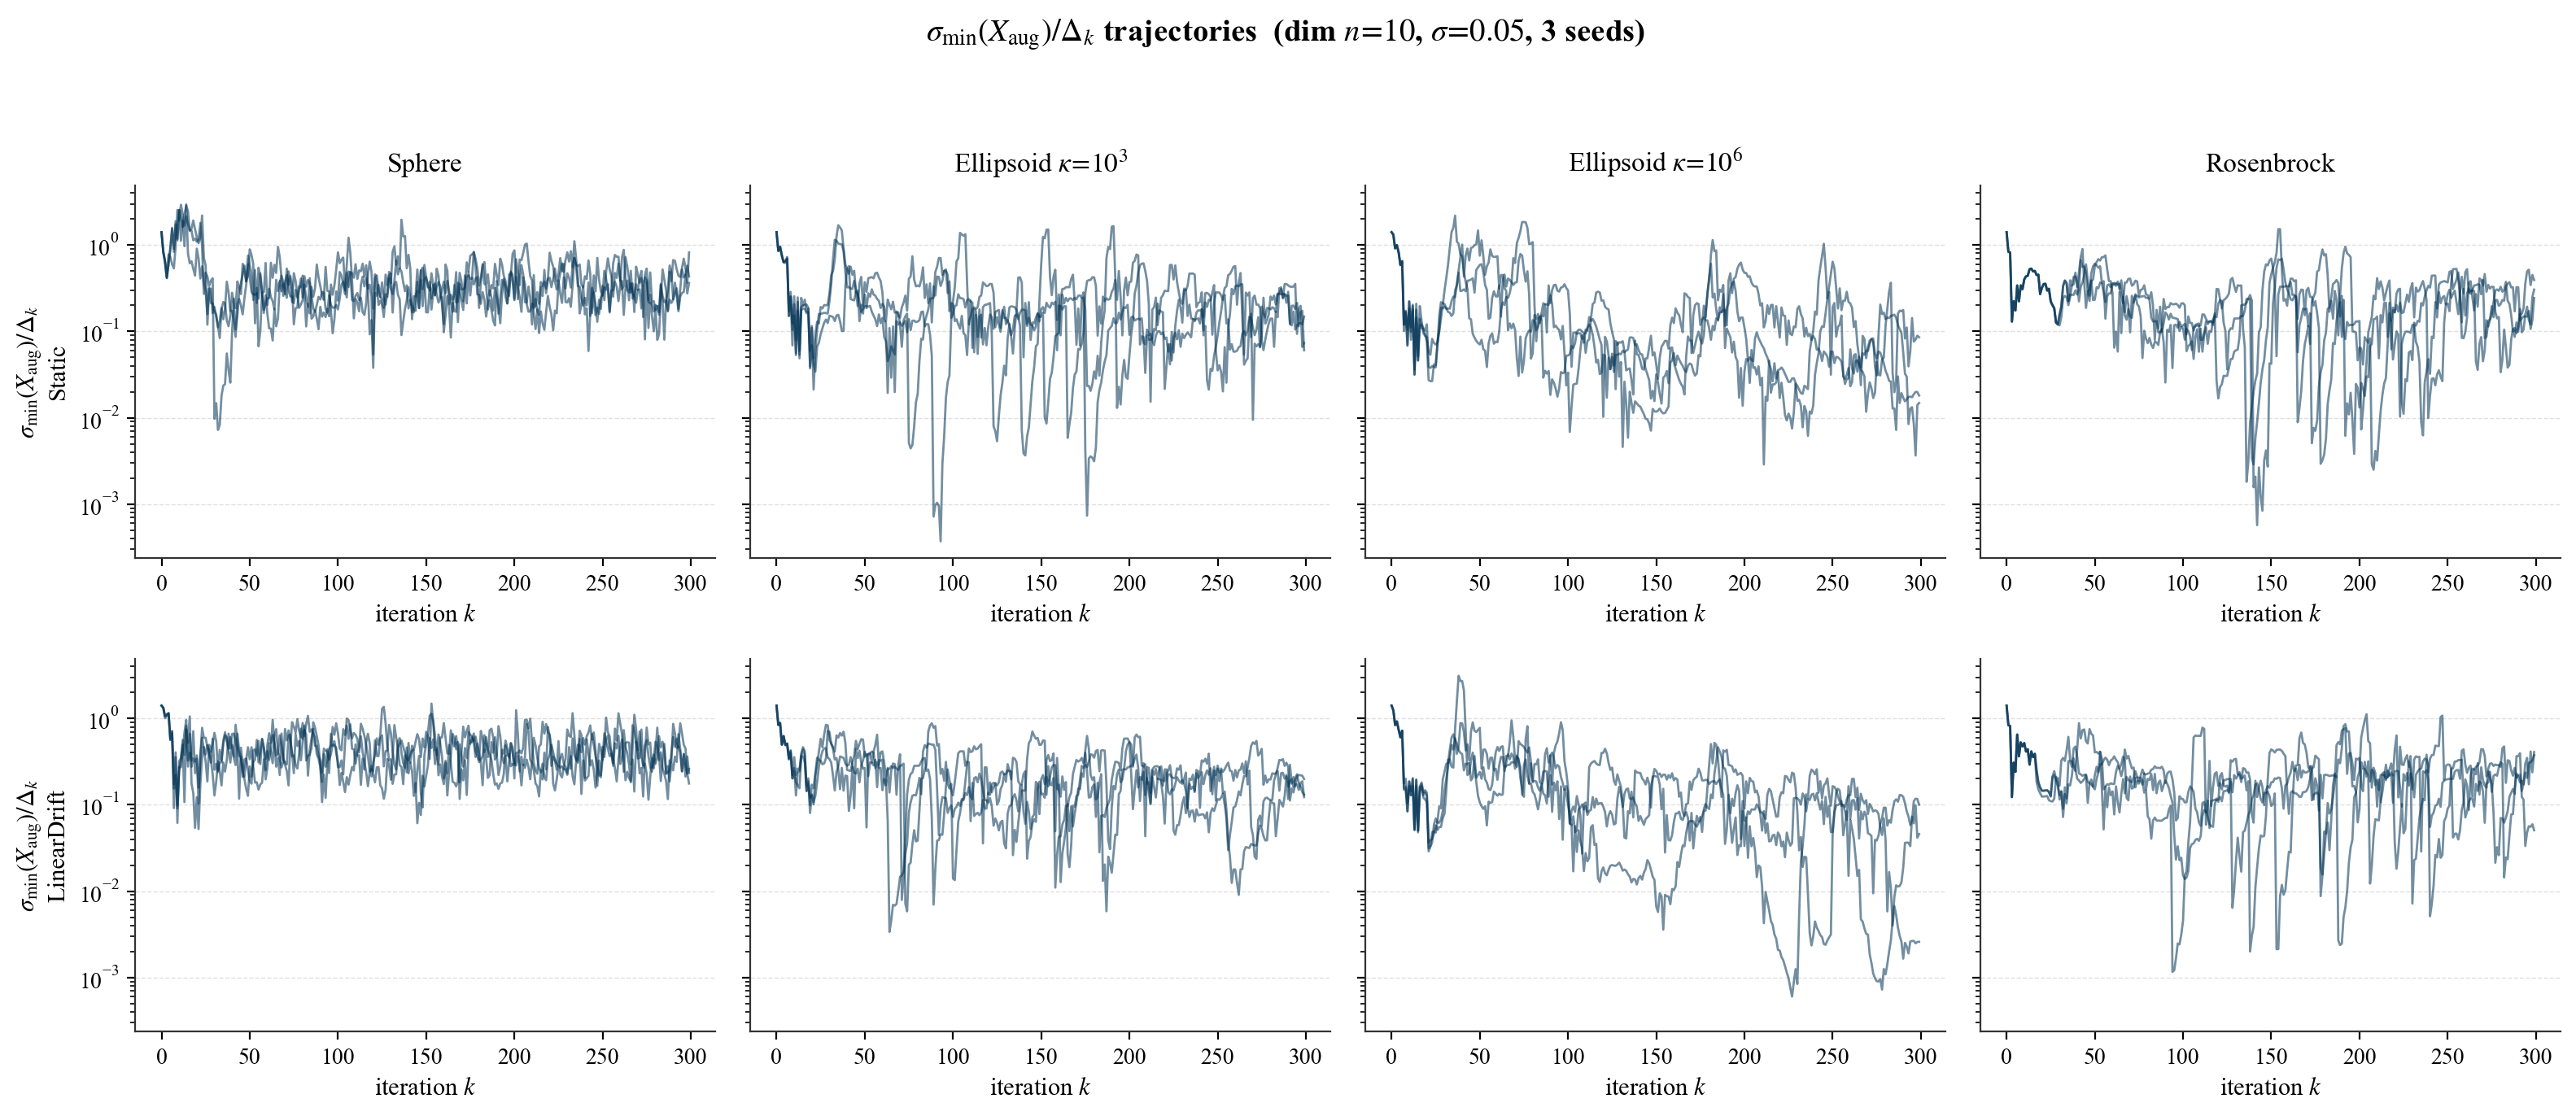
\includegraphics[width=\linewidth]{figures/fig_geometry_trajectories.png}
\caption{Empirical verification of
Assumption~\ref{ass:geometry}: the ratio
$\sigma_{\min}(X_{\mathrm{aug}}^{(k)})/\Delta_k$ along TOBYQA
trajectories. Four representative problems (sphere, ellipsoid
$\kappa=10^3$, ellipsoid $\kappa=10^6$, Rosenbrock), $n=10$,
$\sigma=0.05$, three seeds each, in two environments. The
ratio remains bounded with median $0.21$ and fifth percentile
$0.017$ across $25{,}200$ iterations.}
\label{fig:geometry-empirical}
\end{figure}

% --- 第五部分: 实验结果 ---
\section{Experimental Evaluation}
\label{sec:experiments}

We evaluate TOBYQA on three benchmarks. The Mor\'e--Wild test suite
of $88$ smooth unconstrained functions \cite{MoreWild2009},
wrapped in seven temporal environments and run at three problem
dimensions, gives the main comparison against representative
derivative-free baselines. A $29$-function synthetic suite,
stratified into six curvature regimes, supports a controlled
ablation that isolates the contribution of the two principal
ingredients of TOBYQA: the augmented KKT system with drift unknown
and the affine-scaling subproblem. A hyperparameter sensitivity
study, run on a representative subset of the synthetic suite,
characterizes the robustness of the algorithm to its two
user-facing parameters, the soft-constraint penalty $\rho$ and the
initial trust-region radius $\Delta_0$.

\subsection{Experimental Setup}
\label{sec:exp-setup}

The Mor\'e--Wild suite consists of $88$ smooth unconstrained
problems drawn from the CUTEst collection. We restrict to problems
compatible with each dimension $n \in \{6, 10, 20\}$, use the
standard starting points
$x_0 = \operatorname{linspace}(-1.5, 1.2, n)$, and run $5$ random
seeds per instance. The synthetic suite of $29$ functions is
partitioned by curvature structure into six groups: isotropic
convex ($4$ problems), anisotropic convex ($5$), coupled convex
($5$), weakly nonconvex ($5$), perturbed convex ($5$), and
translated/rotated ($5$). The stratification allows per-group
analysis of which components of TOBYQA contribute on which curvature
regime.

Each problem $f : \R^n \to \R$ is wrapped in seven temporal
environments listed in Table~\ref{tab:envs}. \emph{Static}
preserves the original objective and serves as the no-drift
baseline; the remaining six environments span the drift taxonomy
from purely additive linear drift, the regime in which
Theorem~\ref{thm:linear-drift-decomp} predicts an exact additive
recovery, to chaotic and heteroscedastic perturbations that
violate the algorithmic ansatz. Each environment adds i.i.d.\
Gaussian observation noise of standard deviation $\sigma = 0.1$ in
the main benchmark.

\begin{table}[tbp]
\centering
\caption{Temporal environments used in the Mor\'e--Wild benchmark.
Each wraps the static objective $f(x)$ as
$F(x, t) = E(f(x), x, t) + \mathcal{N}(0, \sigma^2)$.}
\label{tab:envs}
\begin{tabular}{lll}
\toprule
Environment & Form $E(f, x, t)$ & Drift type \\
\midrule
Static        & $f(x)$                                 & none \\
LinearDrift   & $f(x) + 2t$                            & additive linear \\
MultCoupling  & $f(x)\,(1 + 0.005\,t)$                 & multiplicative linear \\
PeriodicAdd   & $f(x) + 5\sin(0.05\,t)$                & additive periodic \\
PeriodicMult  & $f(x)\,(1 + 0.5\sin(0.02\,t))$         & multiplicative periodic \\
ChaoticDrift  & $f(x) + 5\sin(0.07\,t) + 2.5\cos(0.13\,t)$ & multi-frequency \\
Hetero        & $f(x) + 2t + \mathcal{N}(0, \sigma^2(1+0.3\norm{x})^2)$ & linear + heteroscedastic \\
\bottomrule
\end{tabular}
\end{table}

We compare TOBYQA against five baselines spanning the dominant
classes of derivative-free optimization: NEWUOA
\cite{Powell2006NEWUOA}, the canonical trust-region
quadratic-interpolation method on which TOBYQA builds; BOBYQA
\cite{Powell2009BOBYQA}, Powell's bound-constrained extension
applied here without bounds; DFO-LS
\cite{CartisRoberts2019}, a modern noise-aware trust-region DFO
method with its noise-handling option enabled; NMSMAX, an adaptive
Nelder--Mead variant representing the direct-search class; and
Fminunc (BFGS) via SciPy \cite{Virtanen2020} with
finite-difference gradients, included to delineate the failure
mode of derivative-based methods on noisy time-varying problems.

Each algorithm receives a budget of $1500$ function evaluations on
every (problem, environment, seed, dimension) instance. To compare
algorithms on a common metric, every trajectory point is
re-evaluated on the noise-free static $f$, so the reported
optimality gap $\min_t f(x_t) - f^\star$ measures how well each
algorithm tracks the underlying minimizer. We summarize results
through the average rank across (problem, seed) pairs, the
geometric-mean optimality gap in $\log_{10}$ scale, and the
Mor\'e--Wild data profile \cite{MoreWild2009} that gives the
fraction of problems solved to tolerance $10^{-1}$ as a function
of the simplex-gradient budget $\kappa = N_f / (n+1)$.

\subsection{Main Benchmark Results}
\label{sec:main-results}

Figures~\ref{fig:grand-d6}--\ref{fig:grand-d20} report the
Mor\'e--Wild benchmark at $n = 6$, $n = 10$ and $n = 20$. TOBYQA is
the top-ranked method on every (dimension, environment) cell
tested, with average rank ranging from $1.31$ at the most
favorable cell ($n = 6$, LinearDrift) to $2.52$ at the least
favorable ($n = 20$, Static). DFO-LS holds the second rank on
most environments and slightly outperforms NEWUOA in mean
$\log_{10}$ optimality gap. The TOBYQA advantage is modest on
Static---between $0.2$ and $0.4$ orders of magnitude over the
second-place baseline, regardless of dimension---and substantial
on the additive-linear-drift environment, where it reaches
$1.5$ orders of magnitude. The margin narrows on environments
whose drift is nonlinear in time. We unpack the pattern by
dimension below.

\begin{figure}[tbp]
\centering
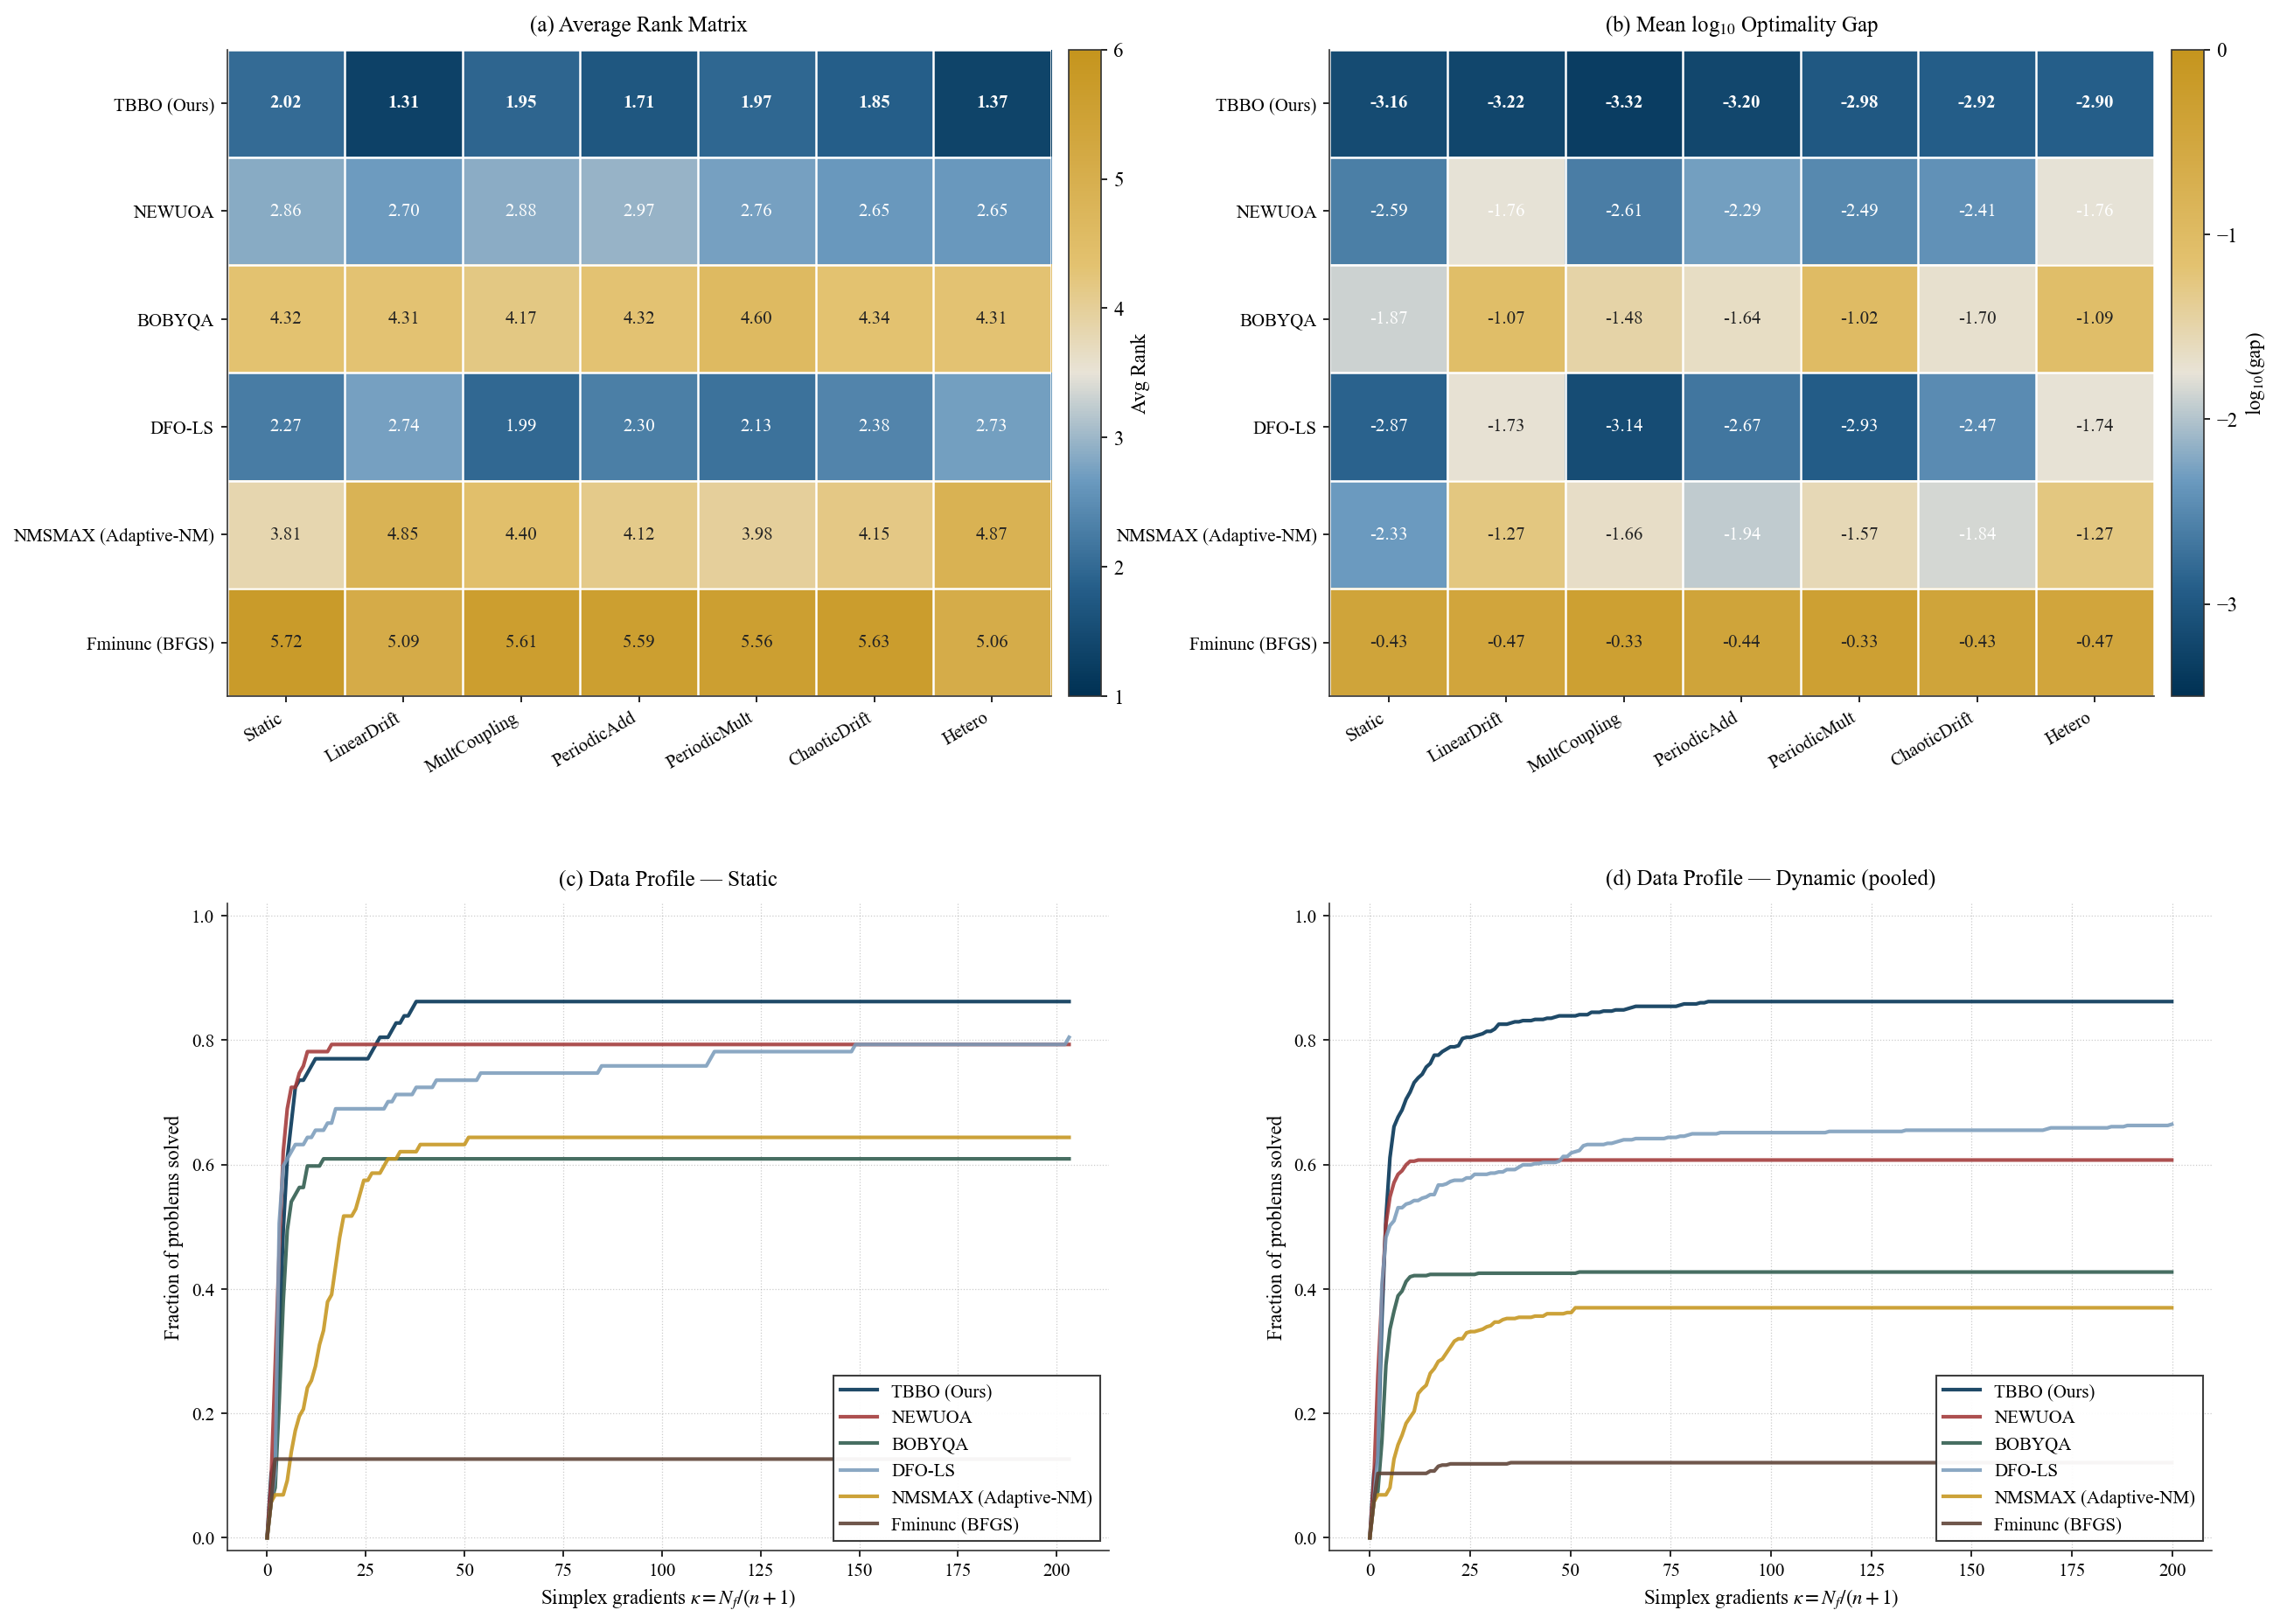
\includegraphics[width=\linewidth]{grand_summary_d6.png}
\caption{Mor\'e--Wild benchmark at $n = 6$. (a) average rank
matrix; (b) mean $\log_{10}$ optimality gap; (c) static-environment
data profile; (d) dynamic-environment data profile pooled over the
six drift settings.}
\label{fig:grand-d6}
\end{figure}

At $n = 6$ (Figure~\ref{fig:grand-d6}), TOBYQA achieves average
rank $2.02$ on Static and between $1.31$ and $1.97$ on the six
drift environments. In mean $\log_{10}$ gap, the Static column
reads $-3.16$ for TOBYQA against $-2.87$ for DFO-LS and $-2.59$ for
NEWUOA, an advantage of $0.3$ orders of magnitude that is
indistinguishable from the trust-region cluster at the low end of
the budget axis (panel c). On LinearDrift the comparison is
$-3.22$ versus DFO-LS $-1.73$ and NEWUOA $-1.76$, a margin of
roughly $1.5$ orders of magnitude. The pooled dynamic data
profile (panel d) shows TOBYQA solving approximately $85\%$ of
problems within the full budget, against $67\%$ for DFO-LS and
$60\%$ for NEWUOA. This separation is the empirical signature of
Theorem~\ref{thm:linear-drift-decomp}: under additive linear
drift, the augmented KKT system absorbs the temporal
contamination of $F_{\mathrm{old}} - F_{\mathrm{new}}$ through
the recovered $\gamma$, so the trust-region update is driven by
the static signal $f(x_k) - f(x_k + s)$ that the baselines have
to reconstruct from drifted observations. The margin narrows
visibly on PeriodicMult ($-2.98$ for TOBYQA versus $-2.93$ for
DFO-LS) and ChaoticDrift ($-2.92$ versus $-2.47$), consistent
with the $L_\mu \tau_{\max}^2$ bias predicted by
Theorem~\ref{thm:nonlinear-drift} when the drift channel has
nonzero second derivative.

\begin{figure}[tbp]
\centering
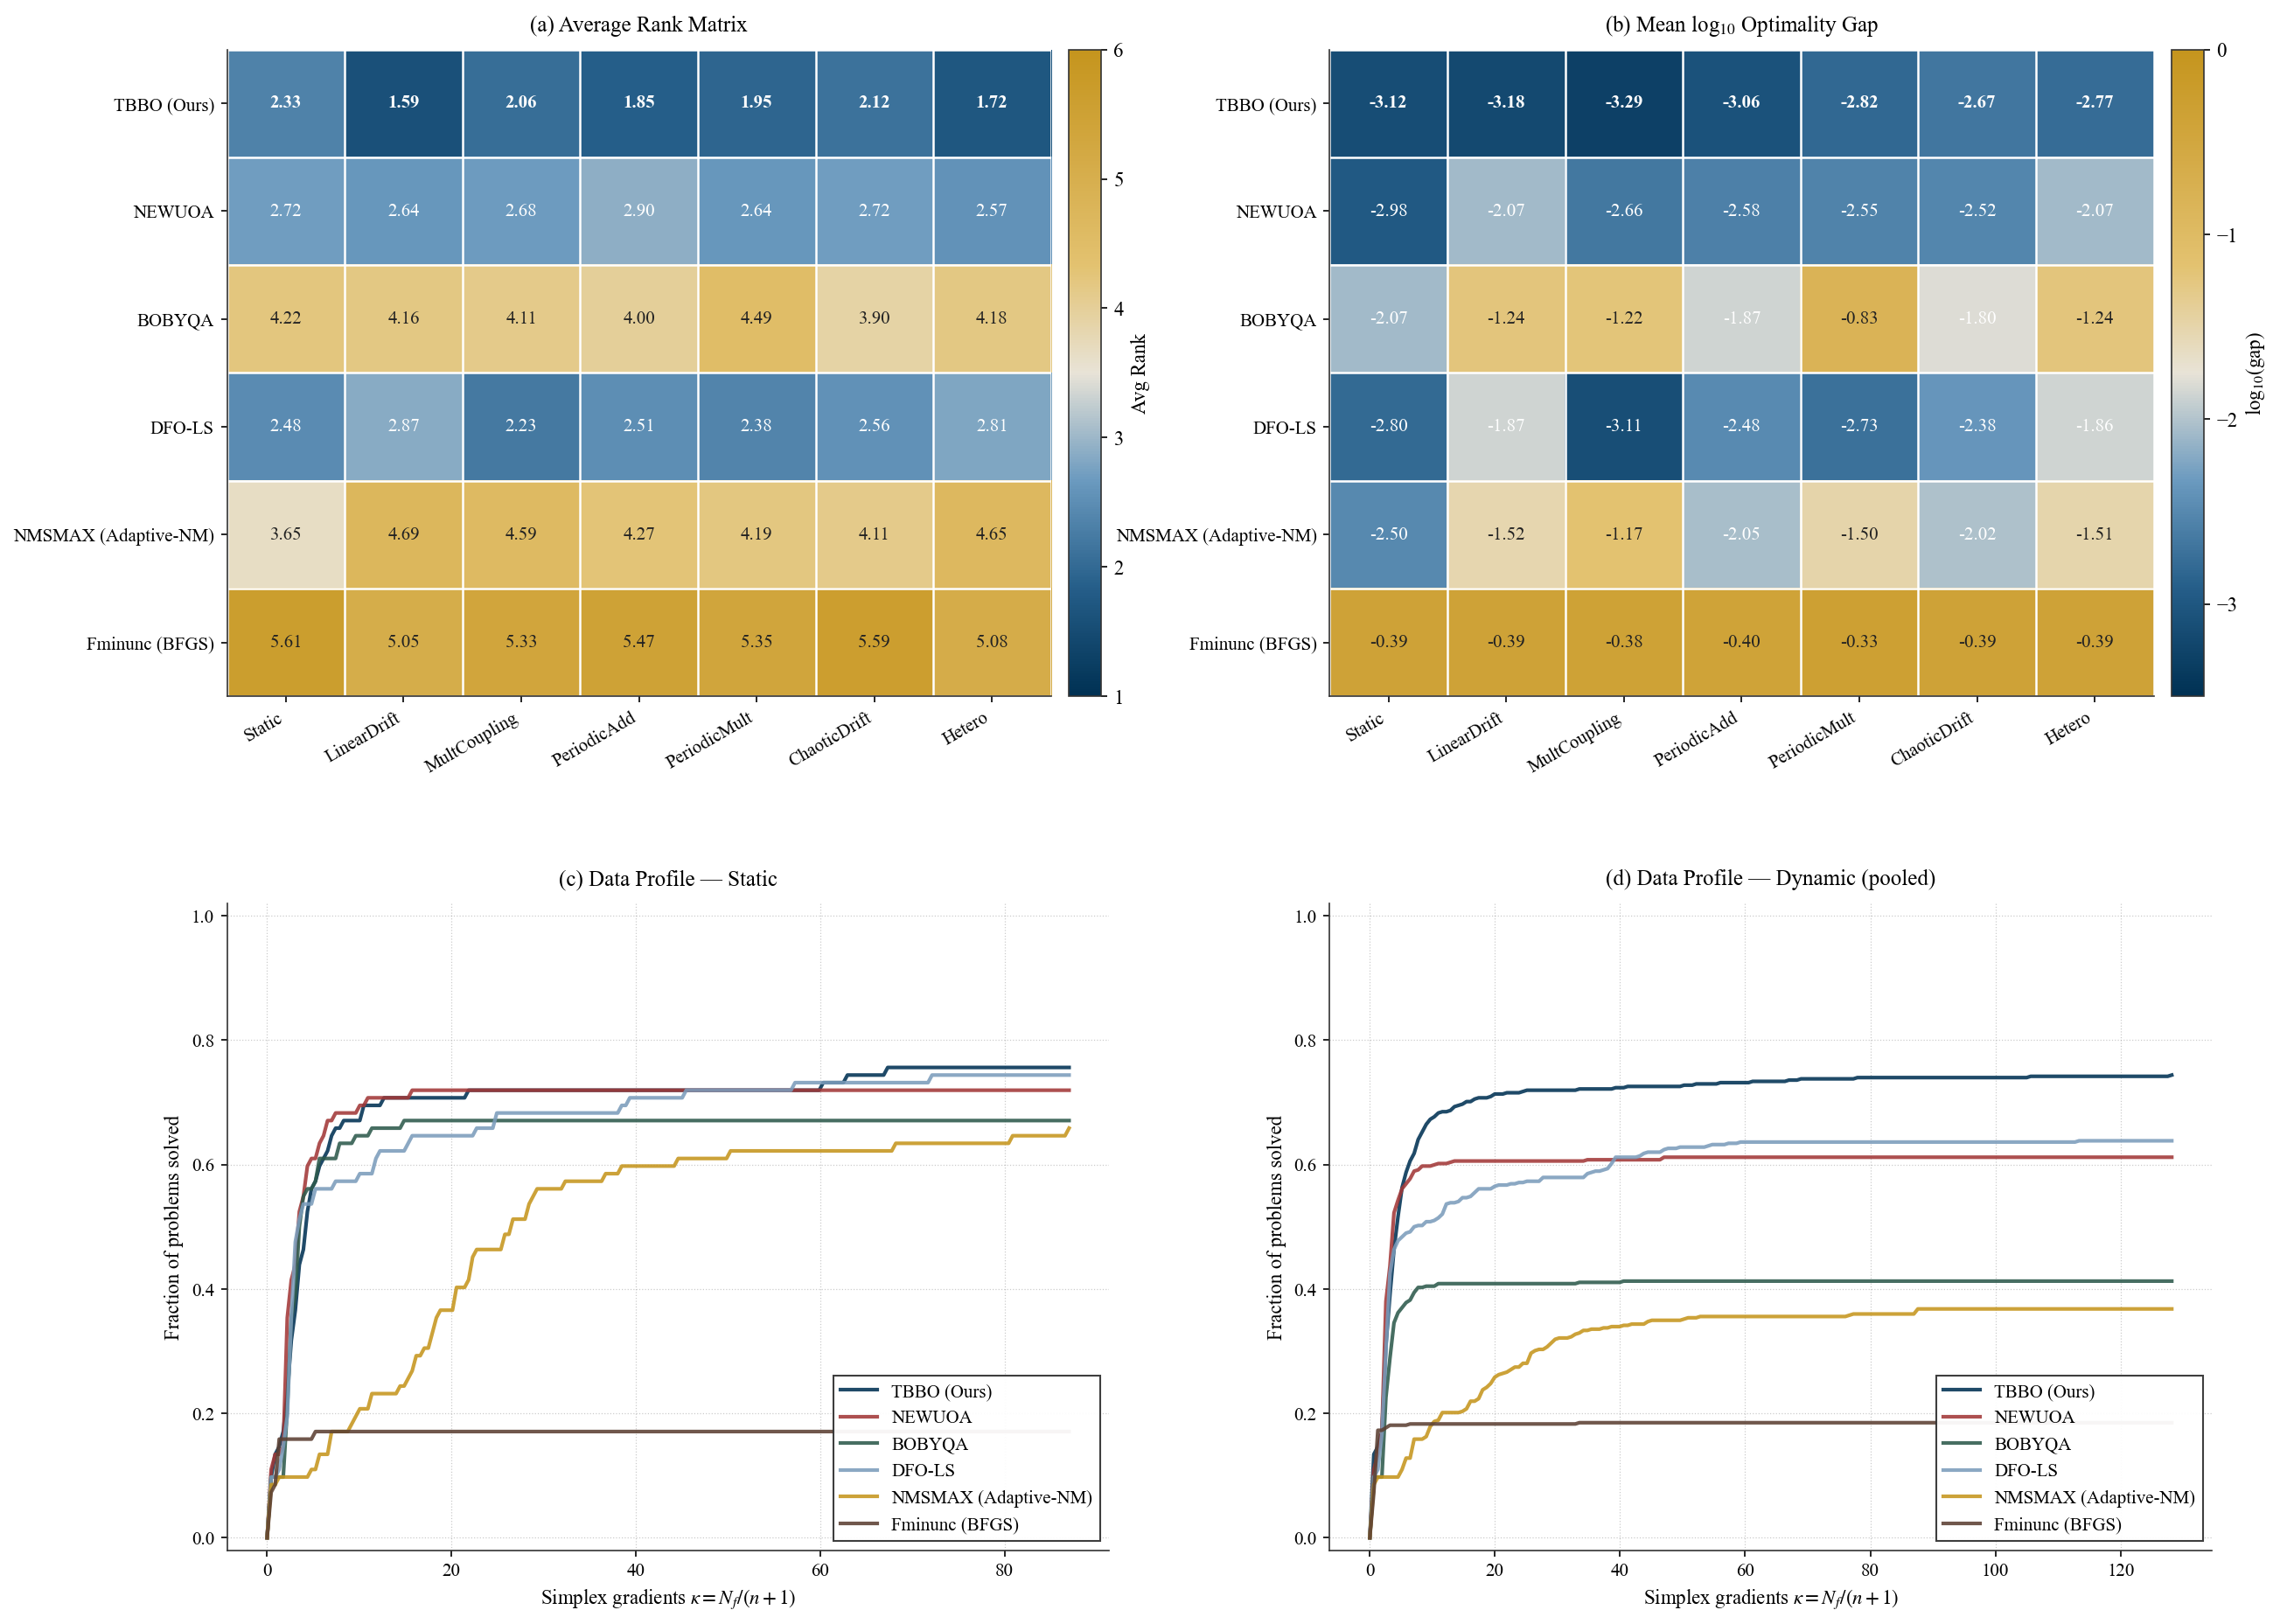
\includegraphics[width=\linewidth]{grand_summary_d10.png}
\caption{Mor\'e--Wild benchmark at $n = 10$. Panels as in
Figure~\ref{fig:grand-d6}.}
\label{fig:grand-d10}
\end{figure}

At $n = 10$ (Figure~\ref{fig:grand-d10}) the picture is
quantitatively similar, with the absolute gaps reduced as the
problem dimension grows. TOBYQA's mean $\log_{10}$ gap is $-3.12$
on Static and $-3.18$ on LinearDrift, against $-2.80$ and $-1.87$
respectively for DFO-LS; the ratio between the LinearDrift and
Static gaps for TOBYQA is essentially unity, confirming that the
drift machinery operates at the same precision as the underlying
quadratic model. The dynamic data profile shows TOBYQA at
approximately $74\%$ solved against $64\%$ for DFO-LS and
$61\%$ for BOBYQA. The relative position of the baselines
shifts: BOBYQA overtakes DFO-LS on the Dynamic profile in this
dimension, while DFO-LS remains stronger on the Static panel.

\begin{figure}[tbp]
\centering
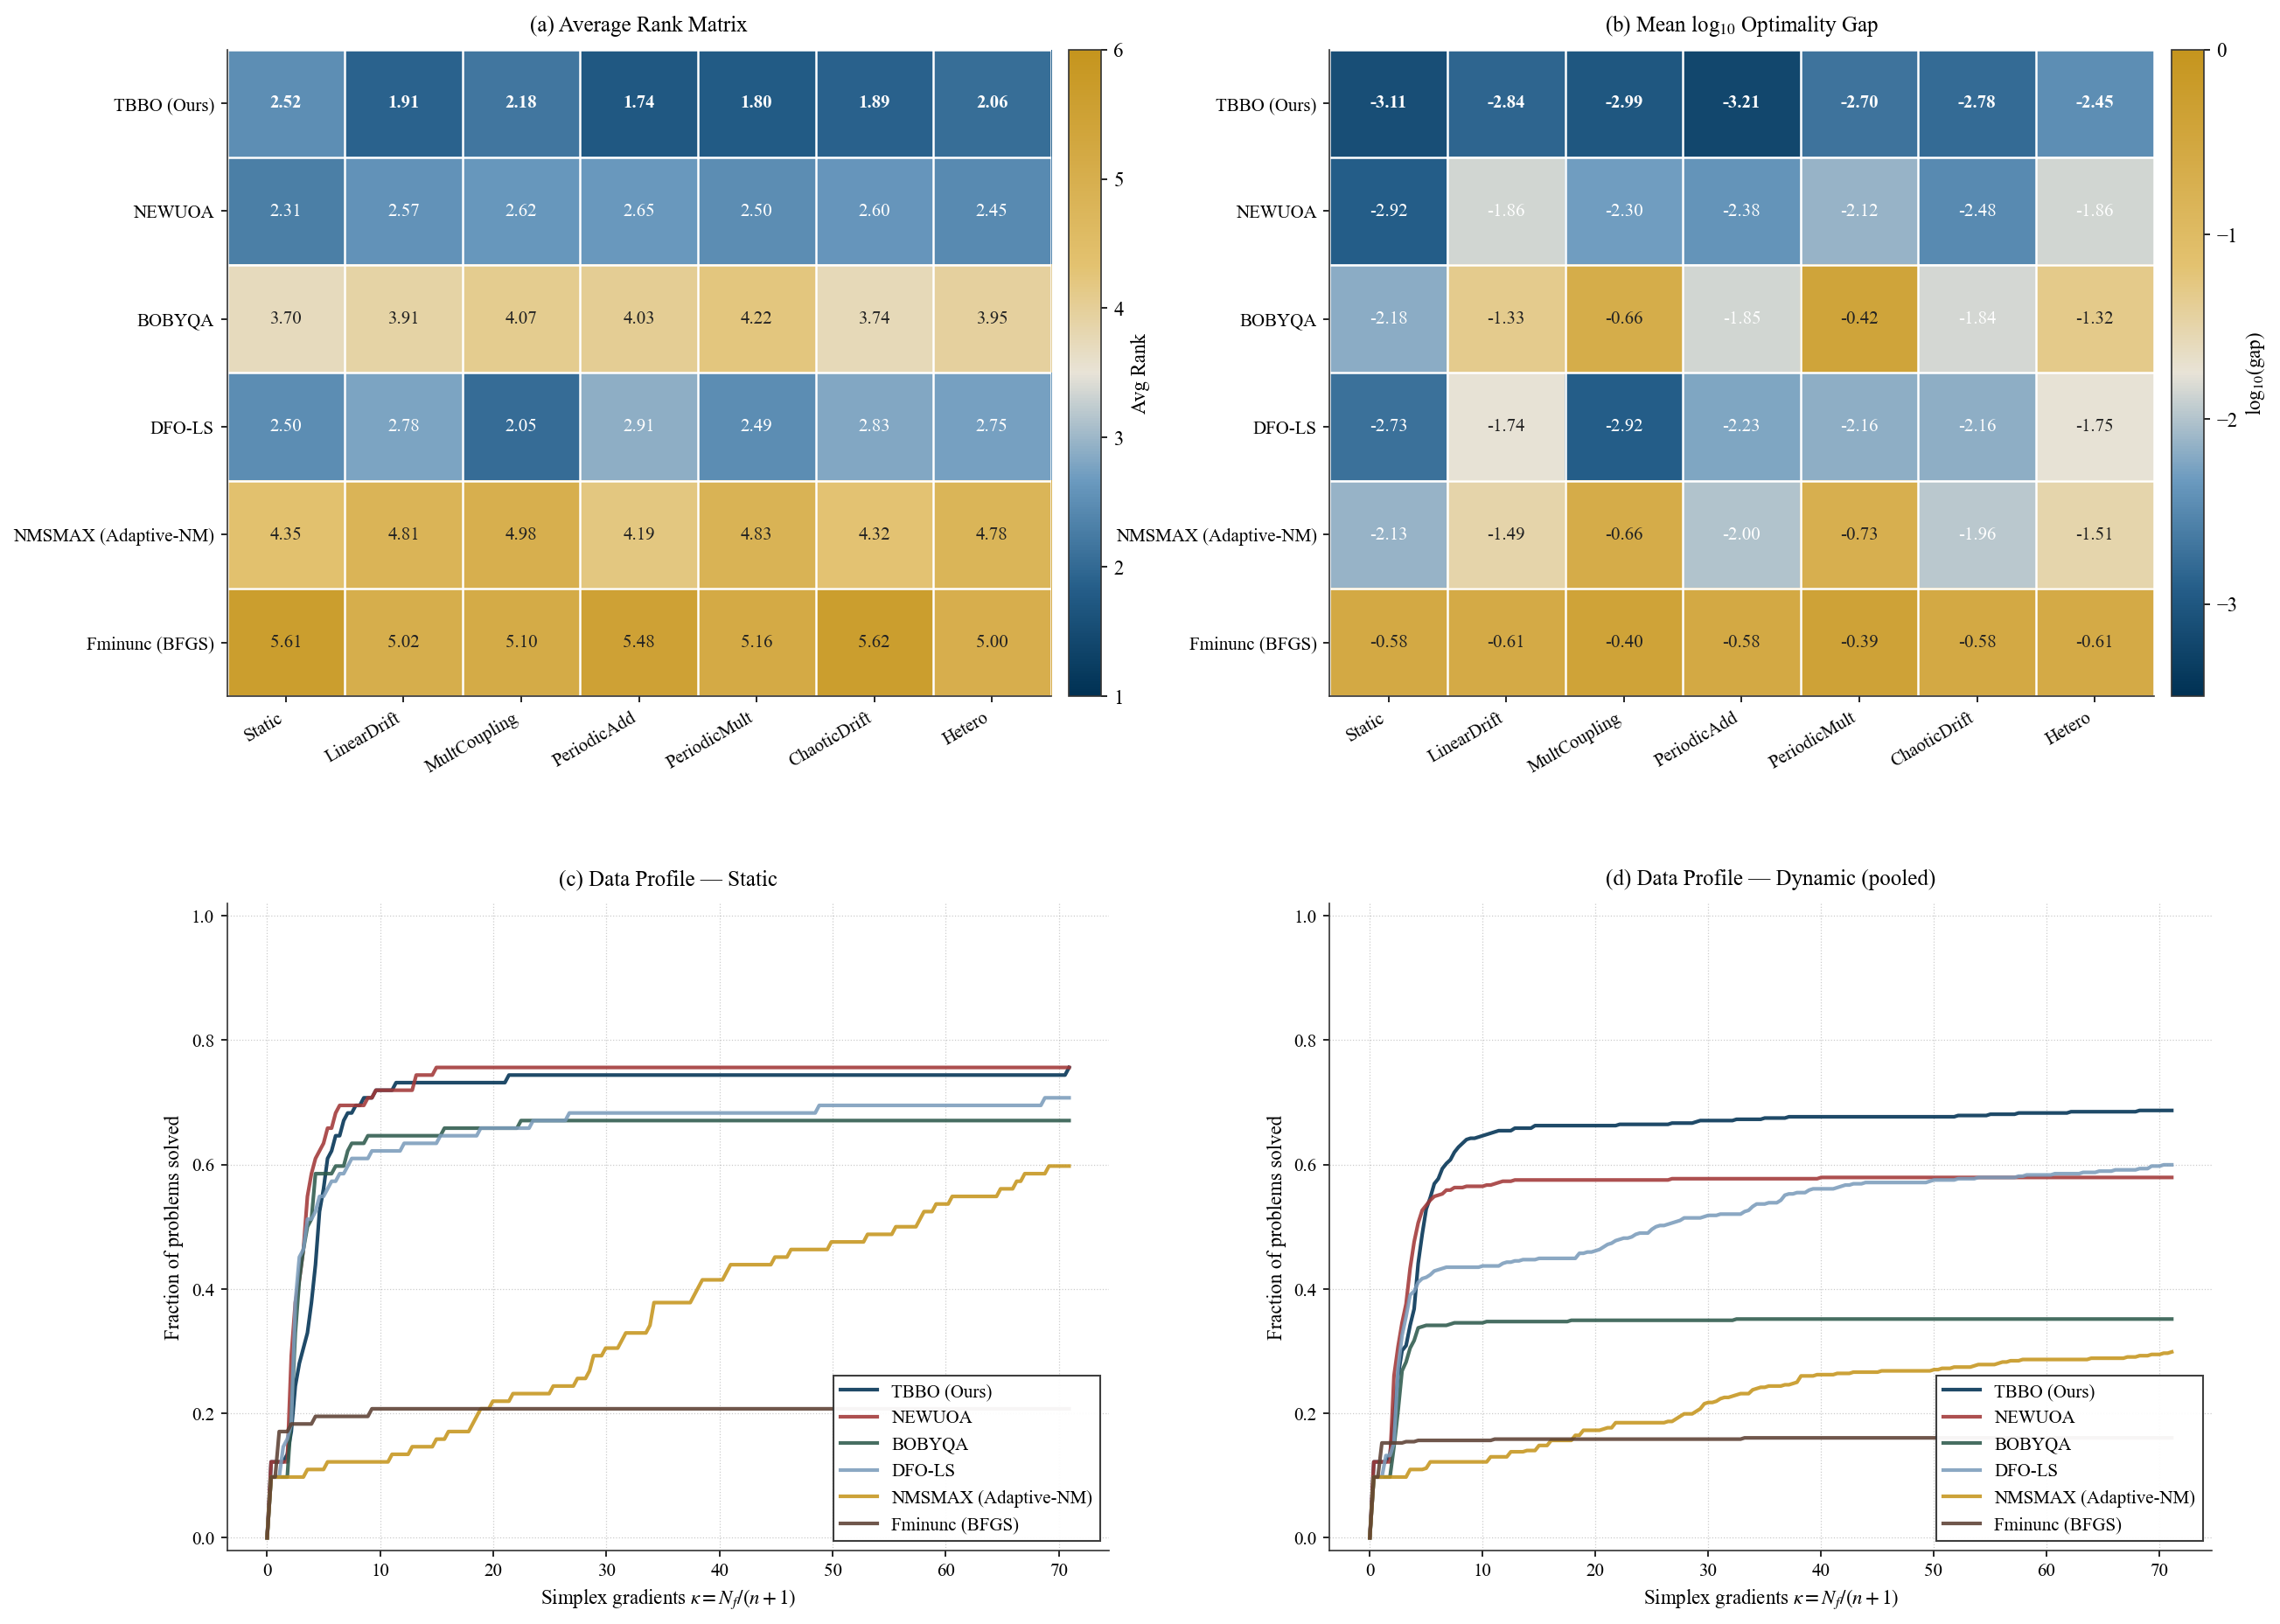
\includegraphics[width=\linewidth]{grand_summary_d20.png}
\caption{Mor\'e--Wild benchmark at $n = 20$. Panels as in
Figure~\ref{fig:grand-d6}.}
\label{fig:grand-d20}
\end{figure}

At $n = 20$ (Figure~\ref{fig:grand-d20}) the dimension reaches
the regime where quadratic-interpolation methods are known to
lose efficiency relative to their low-dimensional behavior, since
the interpolation set size $m = 2n + 1$ becomes a more demanding
fraction of the evaluation budget. TOBYQA retains the top rank on
every environment but the margin compresses: the mean $\log_{10}$
gap on LinearDrift is $-2.84$ for TOBYQA against $-1.74$ for
DFO-LS, $1.1$ orders of magnitude rather than the $1.5$ observed
at $n = 6$. The Dynamic data profile peaks around $0.69$ for
TOBYQA at the budget ceiling, indicating that roughly thirty
percent of problems at this dimension are not fully solved within
$1500$ evaluations by any of the methods tested. The behavior is
not specific to TOBYQA---NEWUOA and DFO-LS show analogous
compression---and reflects the dimensional fade that is a known
characteristic of model-based DFO at this scale.

BFGS with finite-difference gradients solves fewer than $20\%$
of instances at full budget on every dynamic environment, at every
dimension, with mean $\log_{10}$ gap above $-0.5$ throughout. The
gap between BFGS and the derivative-free cluster is the cost of
finite-difference differentiation on a noisy time-varying
landscape.

\subsection{Component Ablation}
\label{sec:ablation}

To isolate the contribution of the two principal ingredients of
TOBYQA---the augmented temporal column $\theta$ together with the
drift unknown $\gamma$ (the \emph{DriftModel}), and the diagonal
affine-scaling transformation of Section~\ref{sec:affine-coords}
(the \emph{AffineScale})---we run a controlled ablation on the
$29$-function synthetic suite. Four variants are compared: the
full algorithm, two single-component leave-one-out variants
($-$DriftModel and $-$AffineScale), and the combined ablation
($-$Drift\&AS) that disables both mechanisms simultaneously. Each
(problem, environment, variant) is run with $3$ seeds at
$\sigma = 0.1$ and dimensions $n \in \{6, 10\}$. We report the
geometric-mean optimality gap with bootstrap $95\%$ confidence
intervals and the Wilcoxon signed-rank $p$-value against Full,
paired at the problem level.

\begin{figure}[tbp]
\centering
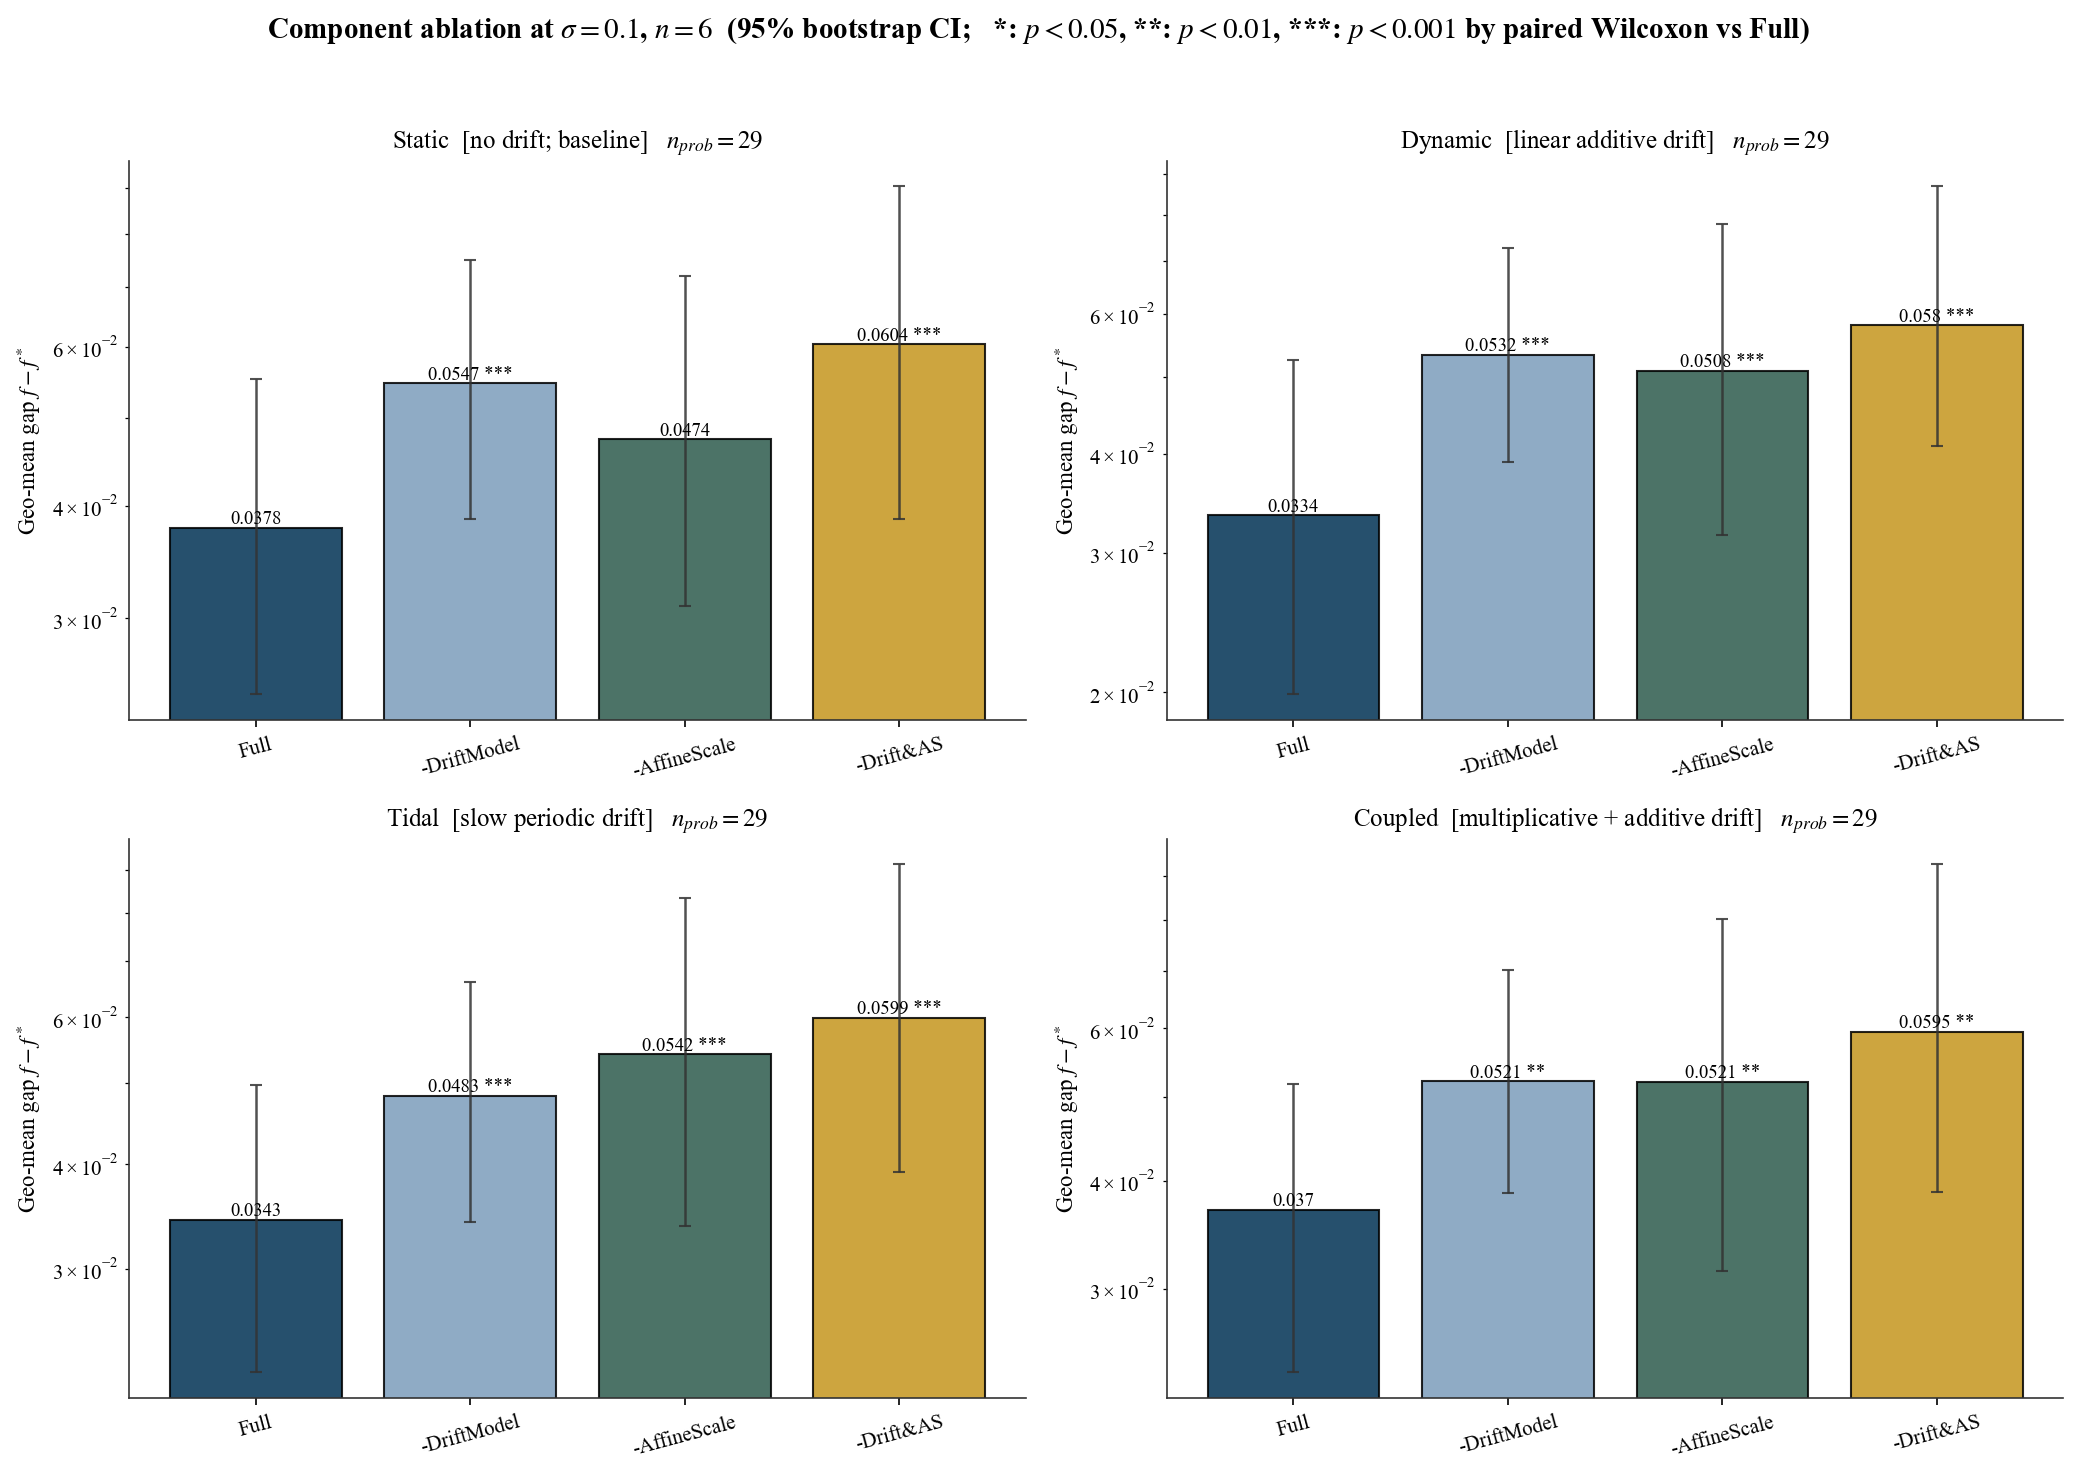
\includegraphics[width=\linewidth]{ablation_d6.png}
\caption{Component ablation at $n = 6$, $\sigma = 0.1$, $29$
problems. Bars show the geometric-mean optimality gap with
bootstrap $95\%$ CI; significance markers report Wilcoxon
signed-rank $p$-values paired against Full at the problem level
($\ast: p < 0.05$, $\ast\ast: p < 0.01$,
$\ast\ast\ast: p < 0.001$).}
\label{fig:ablation-d6}
\end{figure}

\begin{figure}[tbp]
\centering
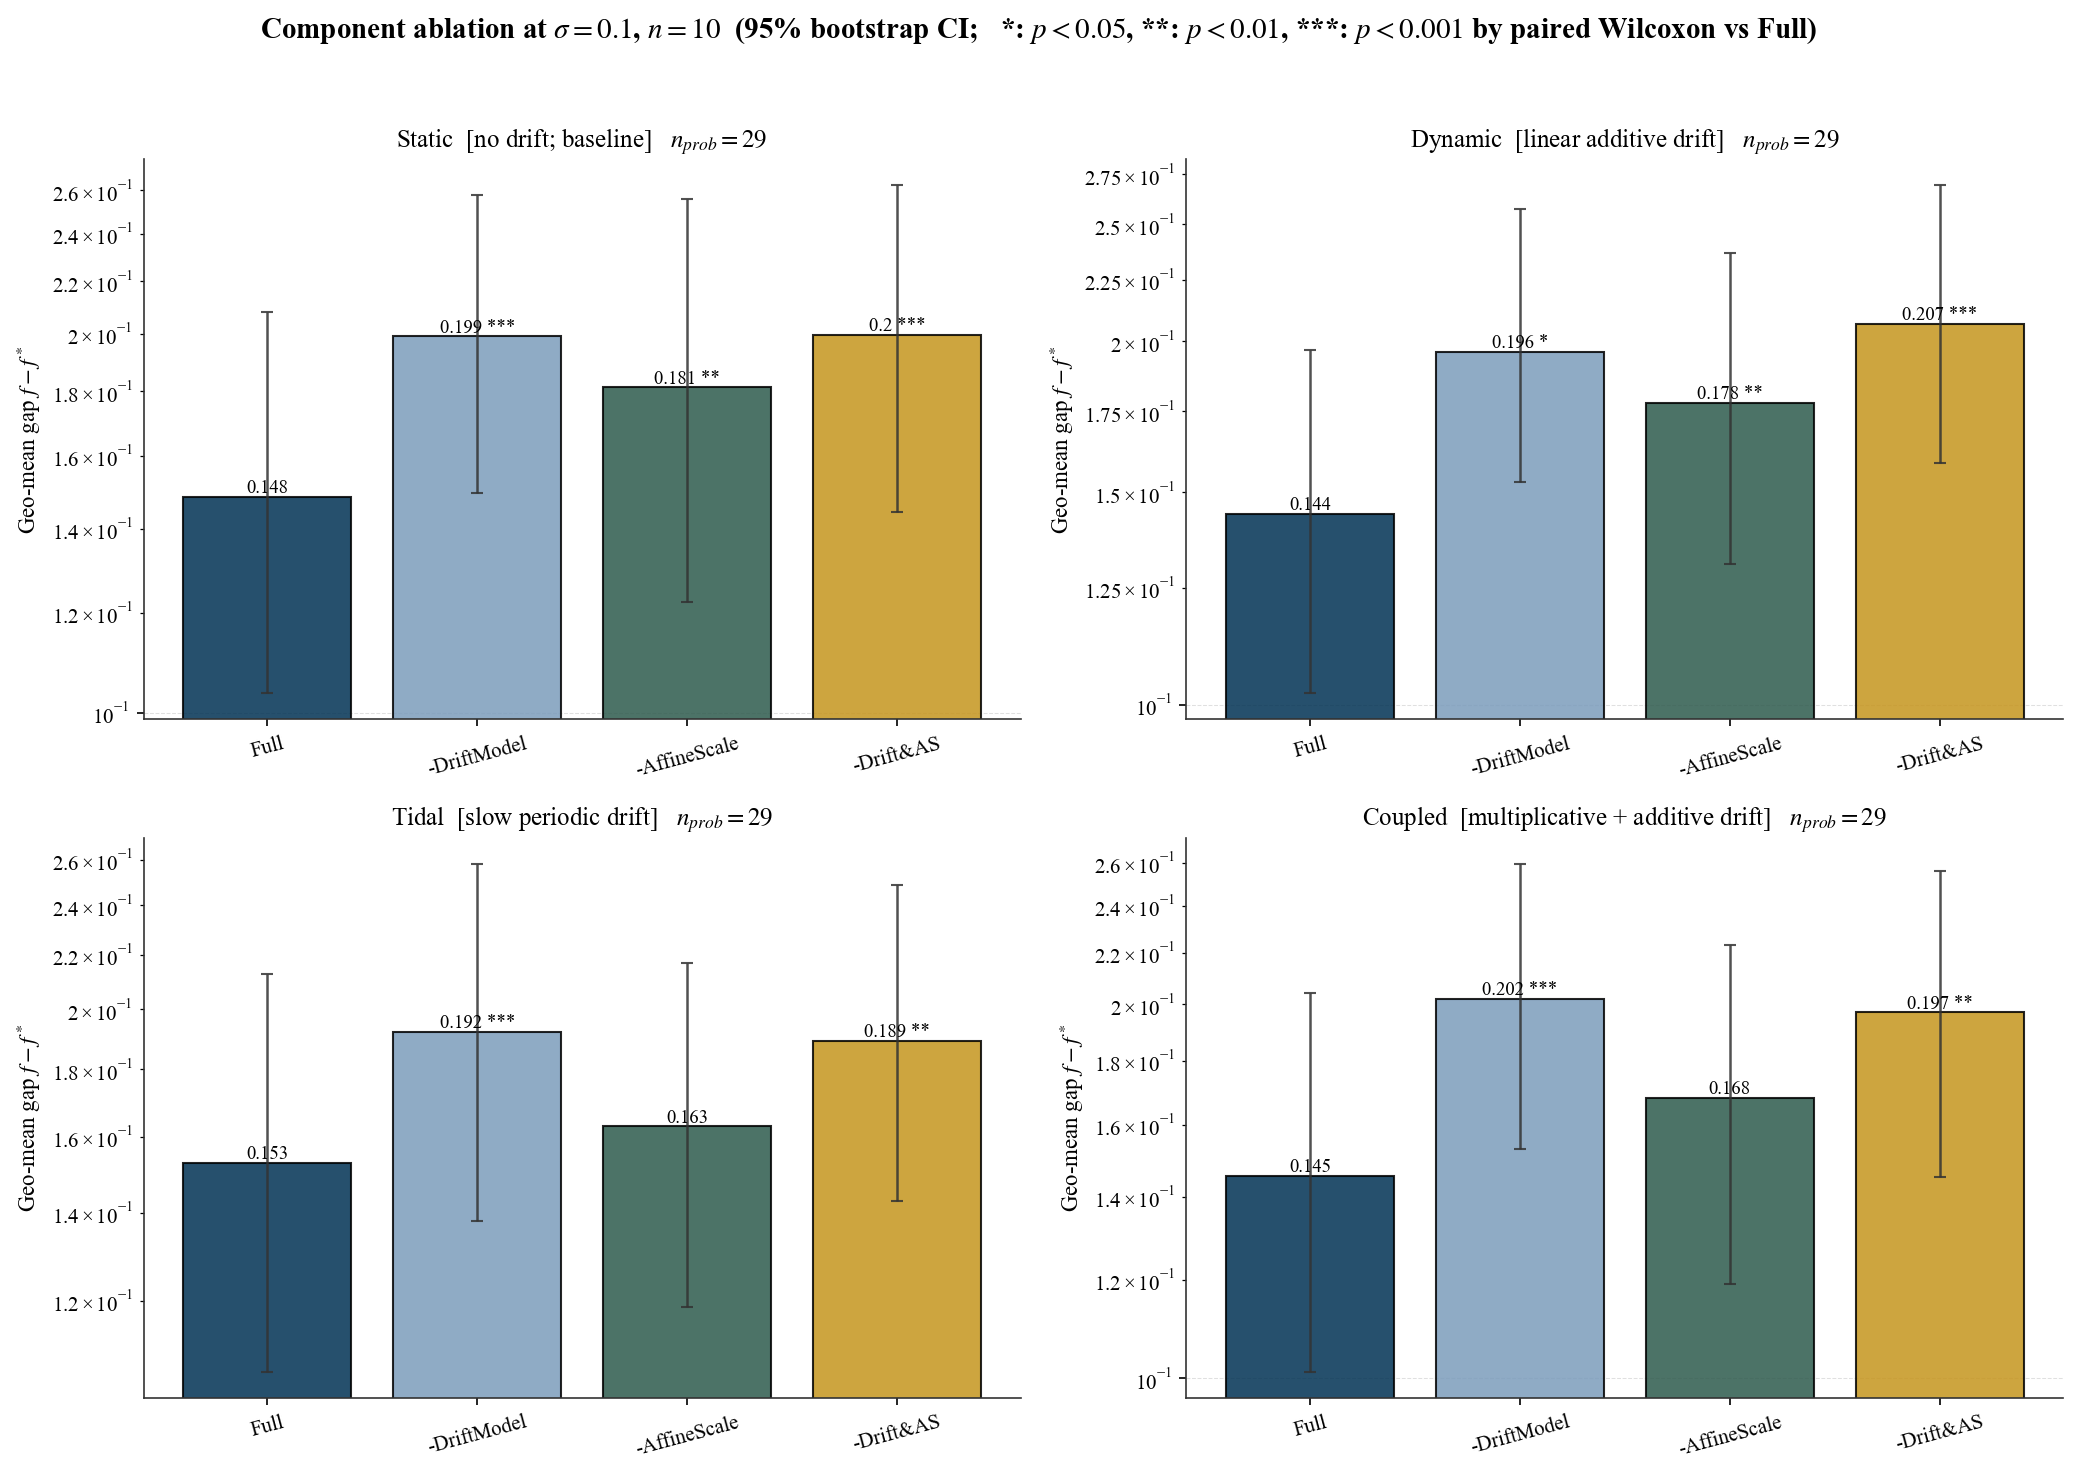
\includegraphics[width=\linewidth]{ablation_d10.png}
\caption{Component ablation at $n = 10$, otherwise as
Figure~\ref{fig:ablation-d6}.}
\label{fig:ablation-d10}
\end{figure}

At $n = 6$ (Figure~\ref{fig:ablation-d6}), disabling the
DriftModel raises the geometric-mean gap by a factor of
$1.4\text{--}1.6$ across every environment, with $p < 0.001$ on
Static, Dynamic, and Tidal and $p < 0.01$ on Coupled. The Static
column ($+0.017$ gap units, $p < 10^{-3}$) is worth noting: even
on a no-drift problem, the augmented temporal column contributes
significantly, indicating that the joint recovery of $(c, g, G,
\gamma)$ stabilizes the model fit beyond what removing the drift
unknown would suggest. On Dynamic and Coupled the gap rises by
$60\%$, consistent with the prediction of
Theorem~\ref{thm:linear-drift-decomp}: removing the drift unknown
forces the algorithm to interpret the linear-in-$t$ component of
$F$ through the spatial unknowns alone, and the resulting model
fit is correspondingly degraded.

The AffineScale contribution is smaller in aggregate---between
$+0.012$ and $+0.020$ across environments at $n = 6$, significant
on Dynamic, Tidal, and Coupled but not on Static---but the
per-group decomposition (Figure~\ref{fig:ablation-groups-d6})
reveals that AffineScale's contribution is concentrated where the
theory predicts. On the anisotropic-convex group (group B,
$5$ problems with strongly direction-dependent curvature),
removing AffineScale raises the gap from $\sim 0.04$ to
$\sim 0.10$, a factor of $2$--$3$, on every environment. On the
isotropic-convex group (group A, $4$ problems with near-spherical
curvature) AffineScale has nearly no effect. This is the
expected behavior of a diagonal curvature preconditioner: it
delivers its full contribution on problems whose curvature is
genuinely anisotropic, and idles on problems whose Hessian is
already well-conditioned.

\begin{figure}[tbp]
\centering
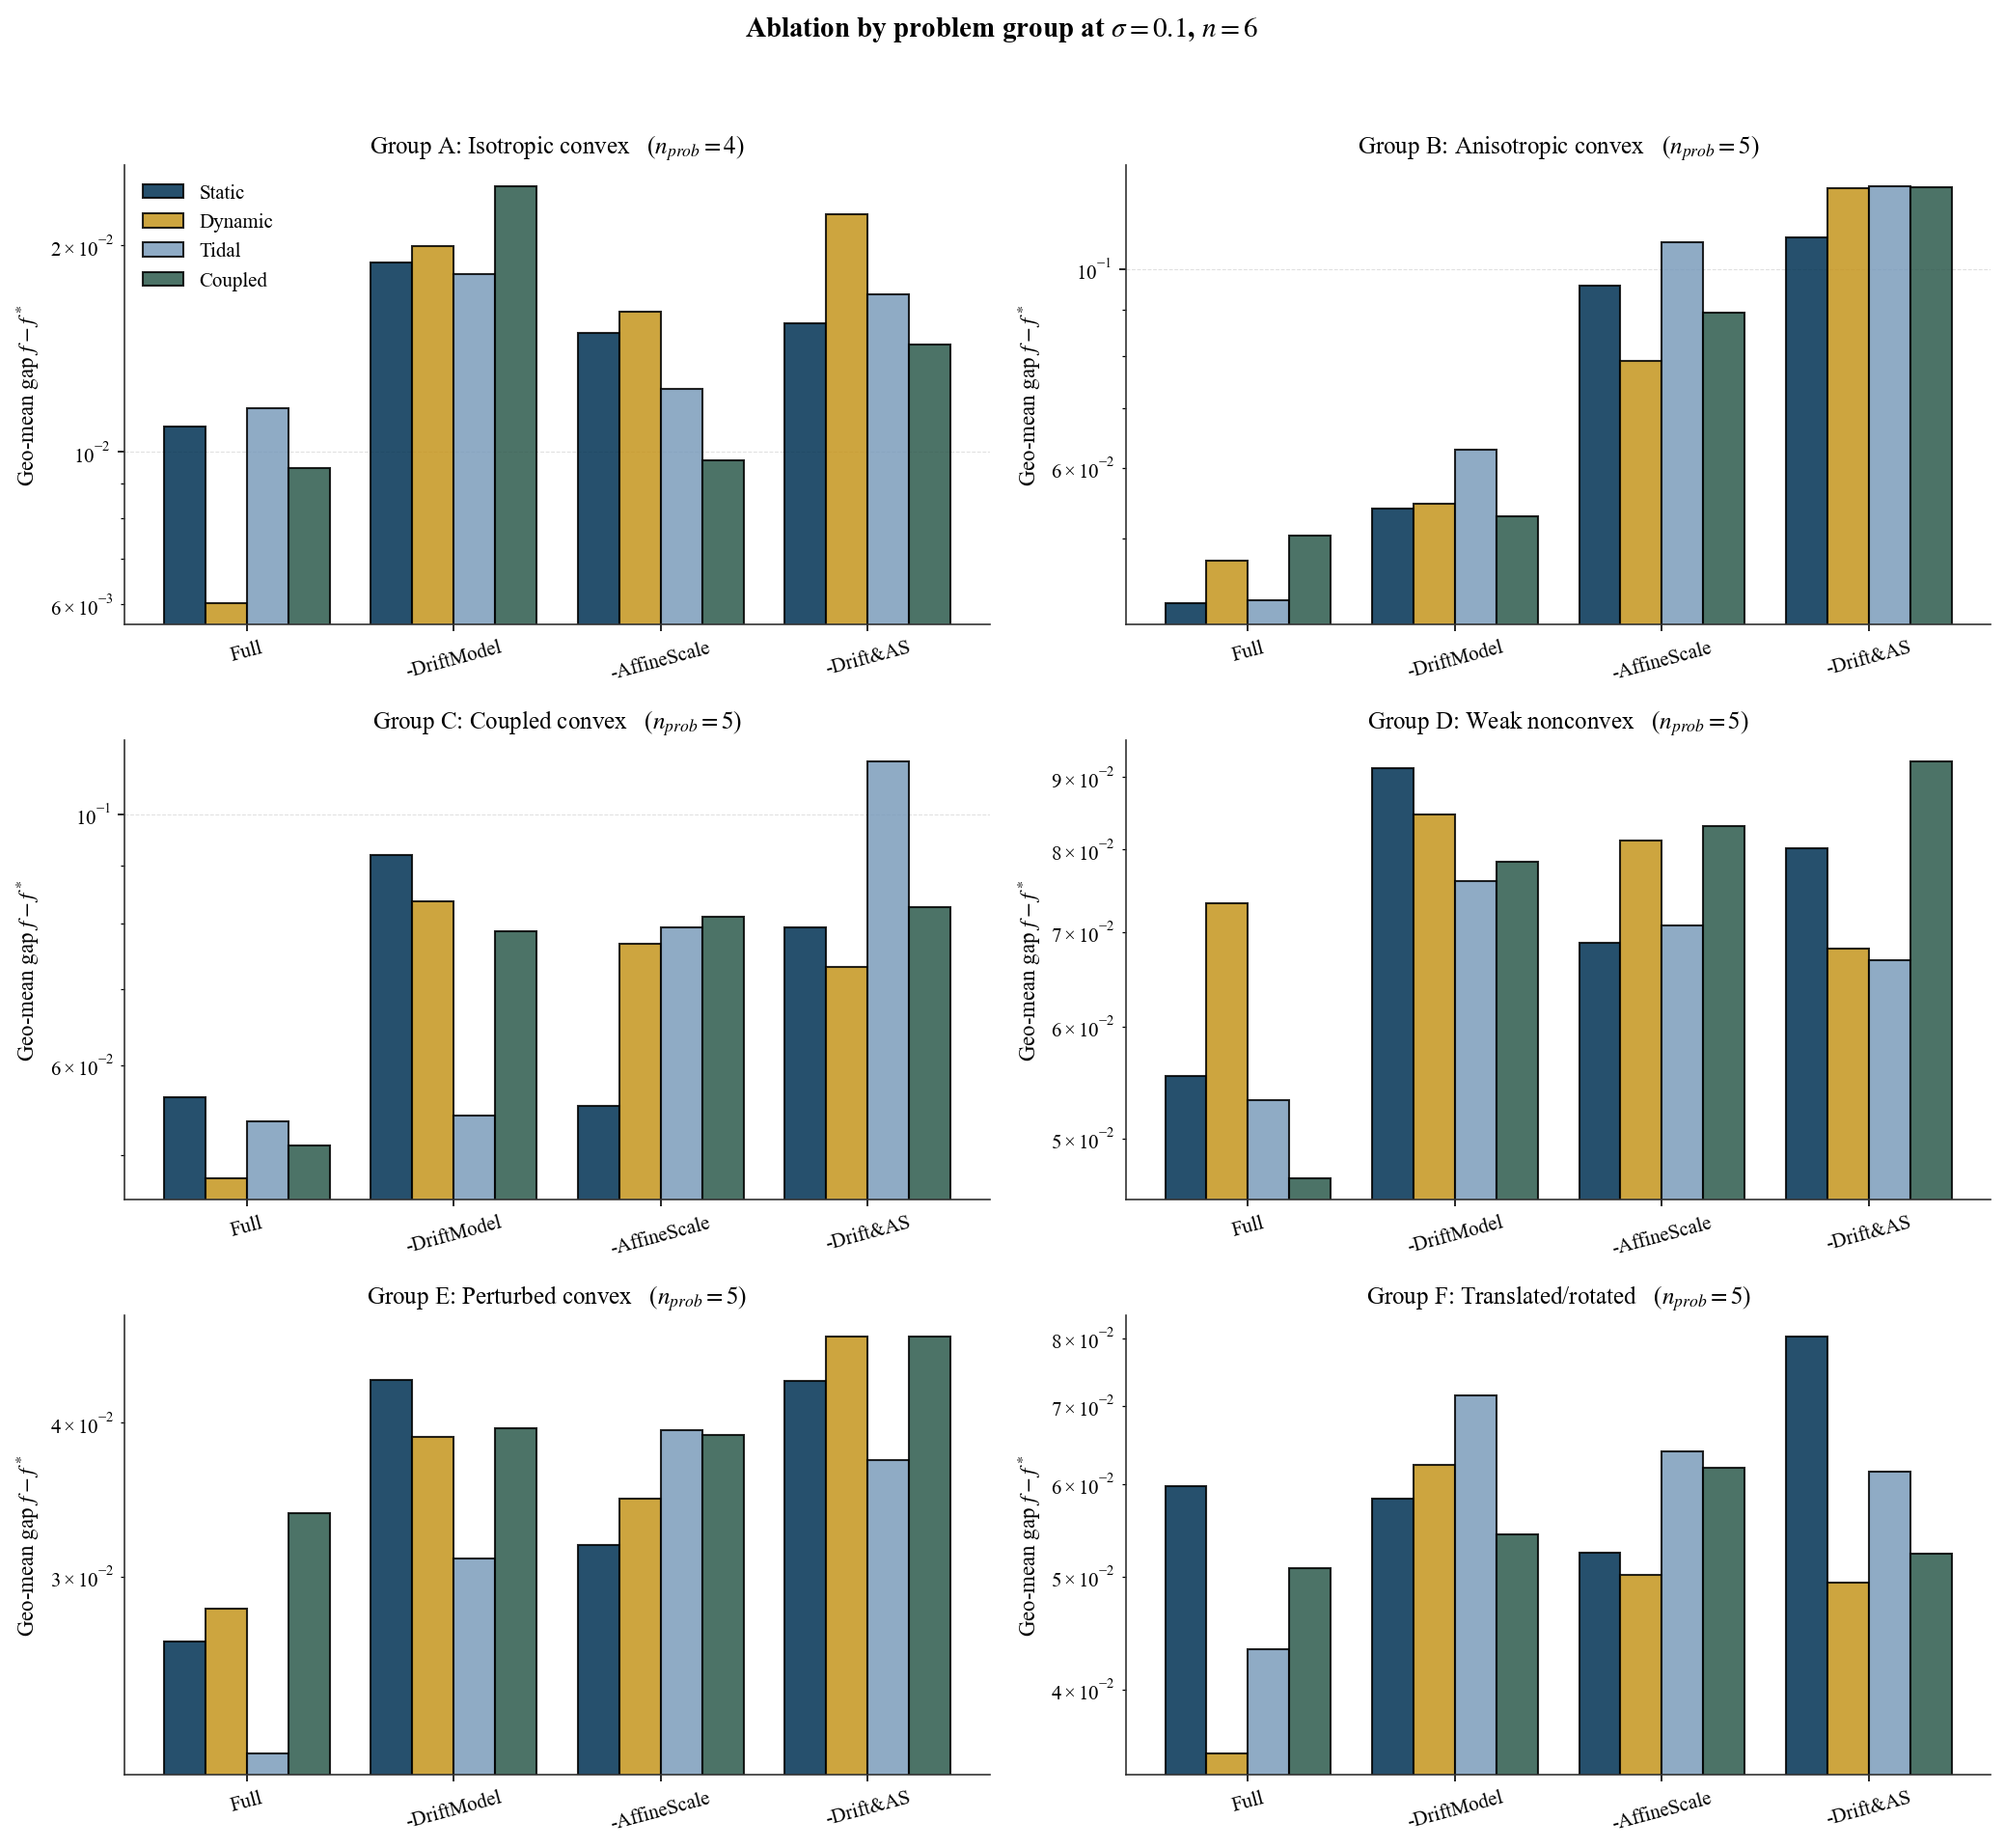
\includegraphics[width=\linewidth]{ablation_groups_d6.png}
\caption{Component ablation broken down by problem group at
$n = 6$. Each panel shows the geometric-mean gap of the four
variants across the four environments (Static, Dynamic, Tidal,
Coupled).}
\label{fig:ablation-groups-d6}
\end{figure}

The combined ablation $-$Drift\&AS produces a degradation
approximately equal to the sum of the two single-component
ablations: at $n = 6$, $0.06$ on Static (versus $0.055$ from
$-$DriftModel and $0.047$ from $-$AffineScale, on a Full baseline
of $0.038$), and similarly on the dynamic environments. The
absence of a strong interaction term indicates that the two
mechanisms operate on orthogonal sources of difficulty: the
DriftModel handles temporal contamination of the observations,
AffineScale handles spatial anisotropy of the curvature, and
neither needs the other to deliver its contribution. Results at
$n = 10$ (Figure~\ref{fig:ablation-d10}) follow the same pattern,
with the AffineScale contribution becoming statistically
significant in more cells---consistent with anisotropy effects
becoming more prominent as $n$ grows.

\subsection{Hyperparameter Sensitivity}
\label{sec:sensitivity}

The algorithm exposes two user-facing parameters: the
soft-constraint penalty $\rho$ and the initial trust-region radius
$\Delta_0$. We characterize the sensitivity of TOBYQA to each
parameter by sweeping it across two orders of magnitude on a
representative subset of the synthetic suite (group A,
isotropic-convex, $4$ problems), at three noise levels
$\sigma \in \{0.01, 0.1, 1.0\}$ and dimension $n = 6$, with $3$
seeds.

\begin{figure}[tbp]
\centering
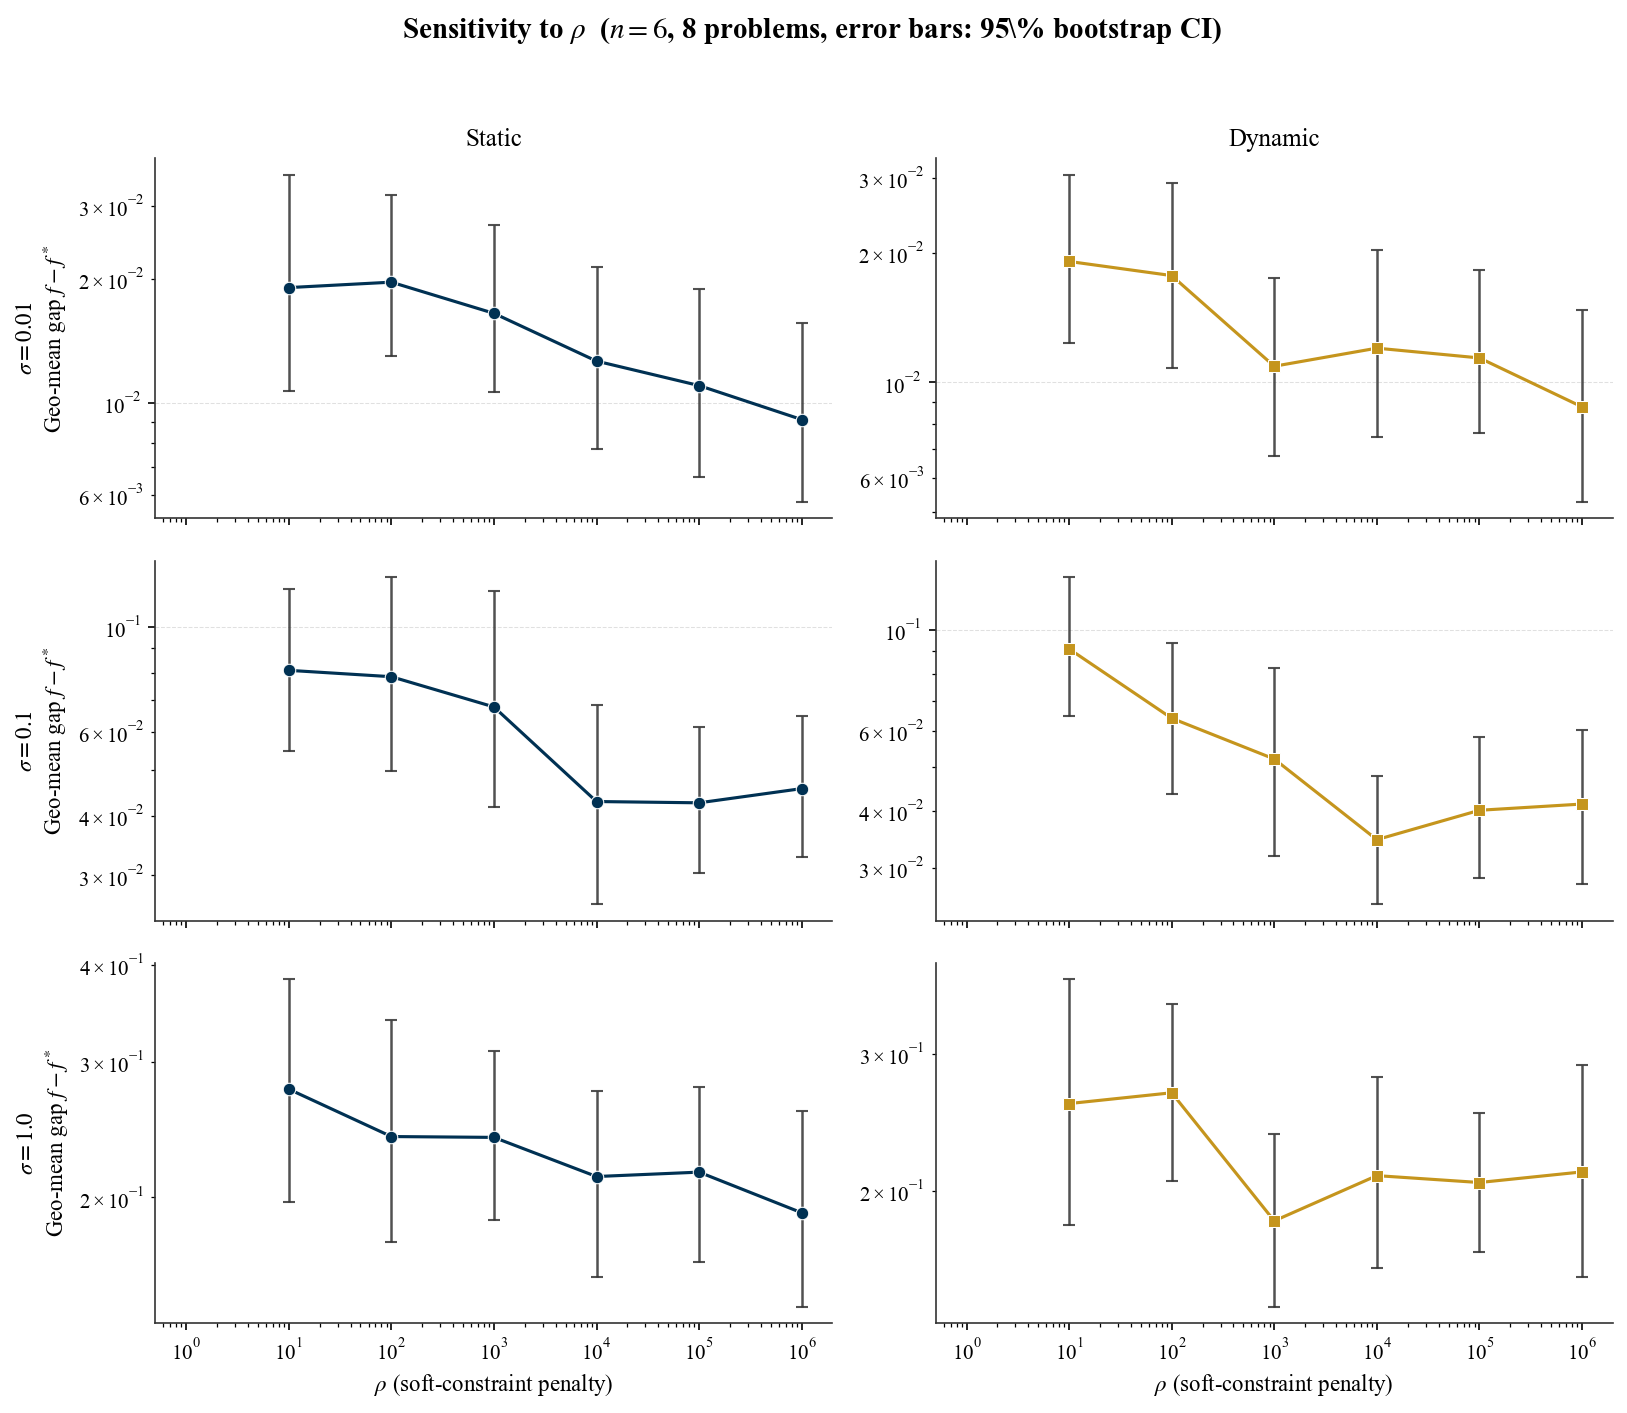
\includegraphics[width=\linewidth]{sensitivity_rho.png}
\caption{Sensitivity to the soft-constraint penalty $\rho$.
Three rows correspond to $\sigma \in \{0.01, 0.1, 1.0\}$; left and
right columns to the Static and Dynamic environments. Error bars
are $95\%$ bootstrap CI.}
\label{fig:sens-rho}
\end{figure}

\begin{figure}[tbp]
\centering
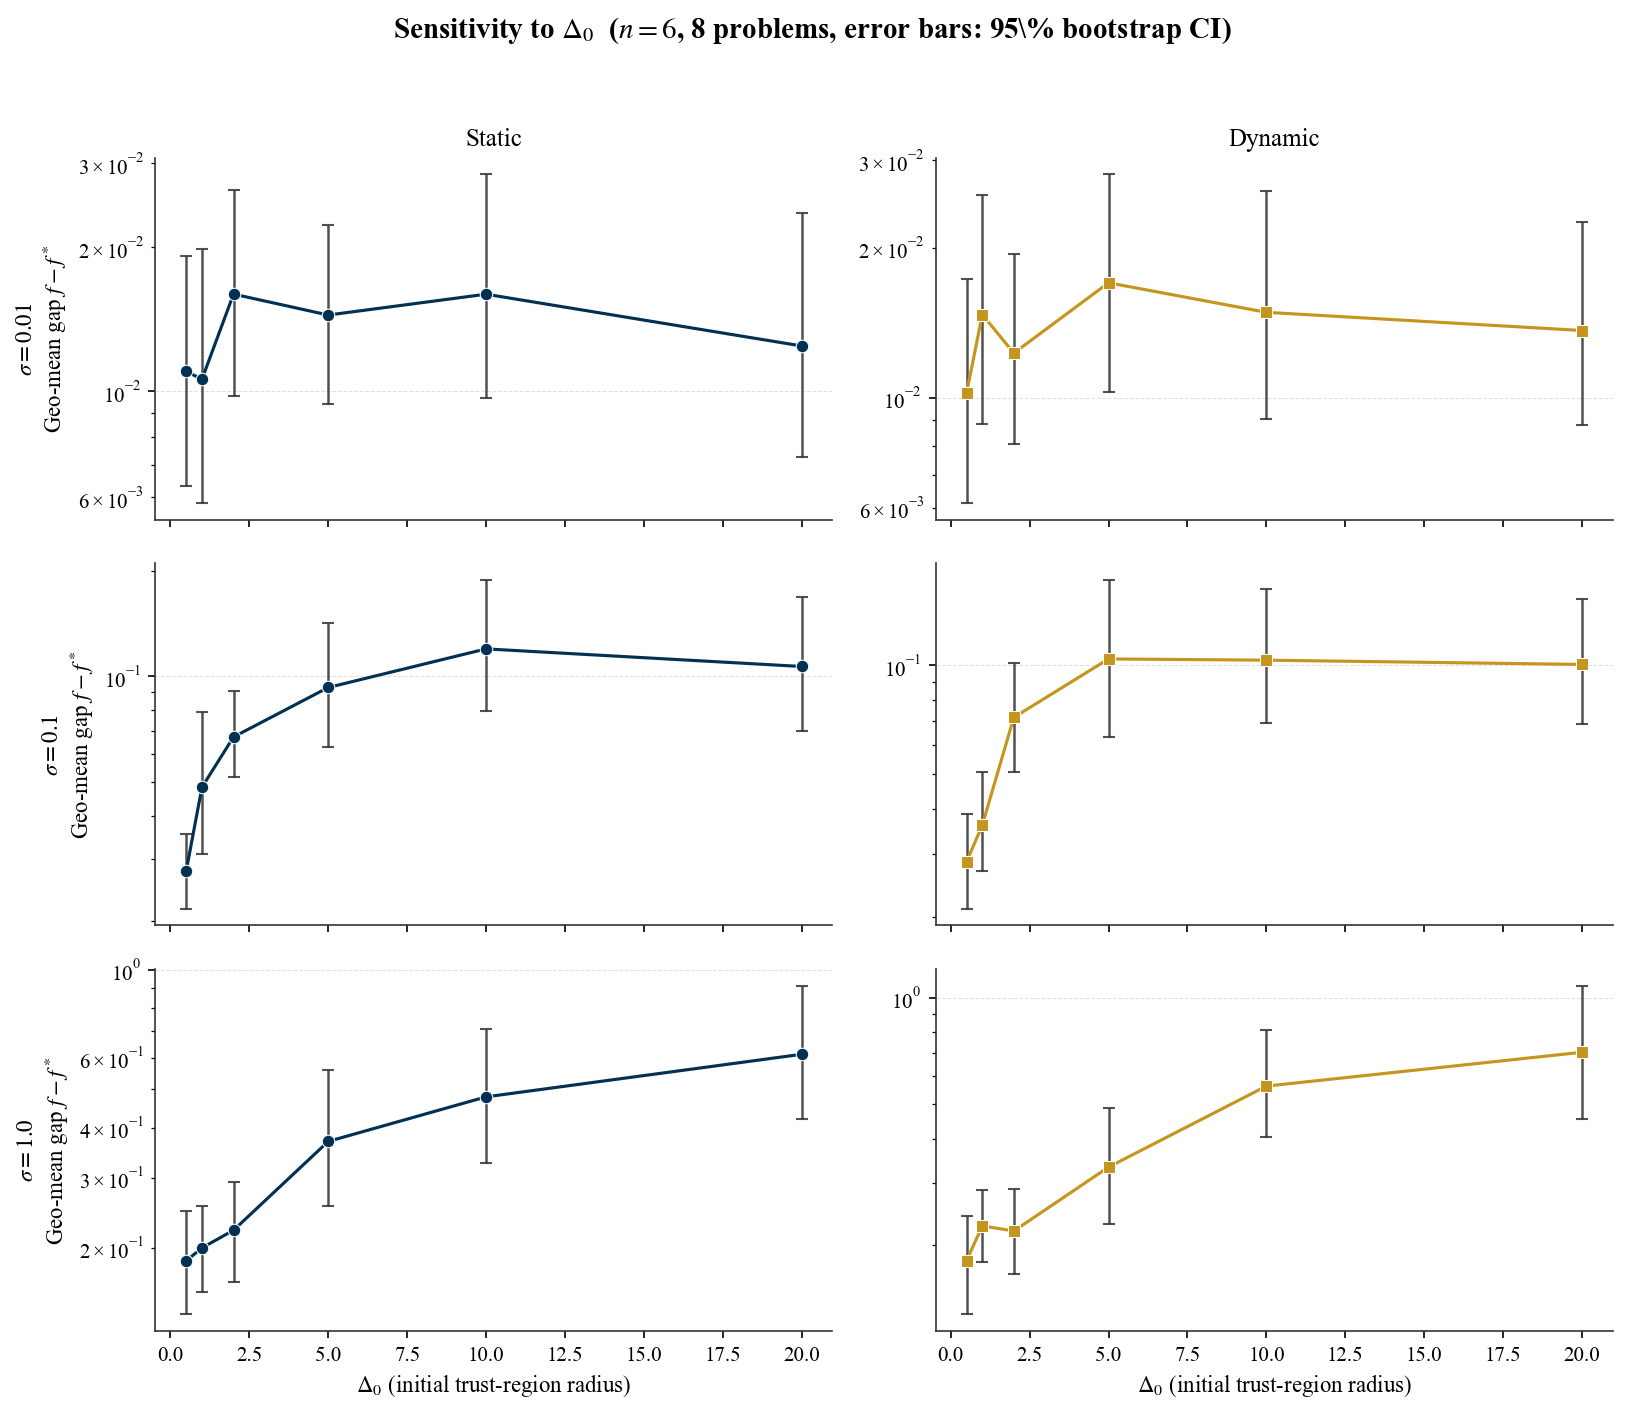
\includegraphics[width=\linewidth]{sensitivity_delta.png}
\caption{Sensitivity to the initial trust-region radius
$\Delta_0$. Panels as in Figure~\ref{fig:sens-rho}.}
\label{fig:sens-delta}
\end{figure}

The dependence on $\rho$ (Figure~\ref{fig:sens-rho}) is
monotonically decreasing across the entire range tested, on both
Static and Dynamic environments at every noise level. The
geometric-mean gap drops by roughly a factor of two between
$\rho = 10$ and $\rho = 10^6$, with most of the improvement
concentrated below $\rho = 10^4$ and a wide plateau above. The
absence of an interior optimum is consistent with the
hard-constraint limit of Proposition~\ref{prop:hard-limit}: at
finite $\rho$ the soft constraint trades a smaller Frobenius norm
of the recovered Hessian against residual fit error, and as $\rho$
grows the latter dominates, pulling the solution toward the exact
interpolation regime. The plateau in $[10^4, 10^6]$ indicates that
the algorithm is robust to the choice of $\rho$ within a wide
range, and any value in this range serves as a reasonable default.

The dependence on $\Delta_0$ (Figure~\ref{fig:sens-delta}) is
noise-dependent. At low noise ($\sigma = 0.01$) the gap is nearly
flat across $\Delta_0 \in [0.5, 20]$. At moderate and high noise
($\sigma = 0.1$ and $\sigma = 1.0$) the optimum lies at the small
end of the range tested: the gap at $\Delta_0 = 0.5$ is roughly
half that at $\Delta_0 = 20$, and the monotone increase is sharp.
The interpretation is that the trust-region machinery contracts
$\Delta_k$ as iterations proceed regardless of $\Delta_0$, but a
large $\Delta_0$ commits more of the early budget to exploration
at radii where the noise-to-signal ratio is unfavorable. Choosing
$\Delta_0 = 1$ as the default is consistent with the small end of
the sensitivity curve on the noise levels of practical interest.

% --- 第六部分: 结论 ---
\section{Conclusion}
\label{sec:conclusion}

We presented TOBYQA, a trust-region method for derivative-free
optimization of noisy time-varying black-box objectives. The
method extends the NEWUOA quadratic-interpolation framework by
augmenting the interpolation system with a linear-in-time column
that introduces a drift unknown $\gamma$ alongside the spatial
unknowns, replacing the hard interpolation constraints with a
soft penalty that absorbs observation noise, and conditioning
the trust-region subproblem in coordinates derived from the
diagonal of the recovered Hessian. The three modifications are
unified within a single augmented KKT system whose closed-form
solution is the central object of the analysis.

The recovery operator $\Pi$ associated with this system admits a
simple algebraic structure: under the column-rank condition,
$\Pi\,\theta = (0,\, 0_n^\top,\, 1)^\top$
(Lemma~\ref{lem:pi-leftinv}). This identity drives the two
recovery results of Section~\ref{sec:theory}. Under additive
linear drift $F(x, t) = f(x) + \beta\,t$, the recovered drift
coefficient decomposes additively as
$\gamma = \gamma^{\mathrm{stat}} + \beta$, where
$\gamma^{\mathrm{stat}}$ is the static-data bias that the same
KKT system would produce in the absence of drift, and the
recovered spatial gradient $g$ is independent of the true rate
$\beta$ (Theorem~\ref{thm:linear-drift-decomp}). Under additive
$C^2$ drift $\mu(t)$, the recovery captures the instantaneous
slope $\mu'(t_k)$ with a curvature-of-drift bias of order
$L_\mu\,\tau_{\max}^2$
(Theorem~\ref{thm:nonlinear-drift}). The exactness of the
linear-drift recovery in the hard-constraint limit
(Corollary~\ref{cor:linear-drift-exact-limit}) is the algebraic
content of the drift-compensated ratio test.

The empirical evaluation supports these recovery results. On the
Mor\'e--Wild benchmark of $88$ problems wrapped in seven temporal
environments, TOBYQA is the top-ranked method across all three
dimensions tested, with a margin of approximately $1.5$ orders
of magnitude in mean $\log_{10}$ optimality gap over the
strongest baseline on the additive-linear-drift environment and
a narrowing margin on environments with nonlinear temporal
structure. The component ablation on a $29$-function synthetic
suite identifies the augmented KKT system as the dominant
contributor under drift, and the affine-scaling transformation
as the dominant contributor on anisotropic curvature, with the
two mechanisms operating on orthogonal sources of difficulty.

Several questions remain open. A tracking error bound for the
iterate $x_k$ relative to the time-varying minimizer requires a
Lyapunov-style propagation argument that goes beyond the
per-iteration recovery results established here. Global
convergence of TOBYQA under the time-priority replacement rule is
not addressed in this work: the classical NEWUOA convergence
theory applies in the static regime under a $\Lambda$-poisedness
maintenance rule, and extending it to the replacement rule
actually used by the algorithm is left for future investigation.
Finally, the linear-in-time temporal column captures only the
local first derivative of the drift channel; enriching it with
polynomial columns
$[\theta,\,\theta^{(2)},\,\dots,\,\theta^{(p)}]$ would extend
the exact-recovery regime to polynomial drift of order $p$ at
the cost of $p - 1$ additional unknowns in the KKT system, and
the trade-off between fidelity and conditioning of the enlarged
system is a natural direction for further work.

% ...
% ============================================================
\begin{thebibliography}{99}
\bibitem{Powell2006NEWUOA}
M.~J.~D. Powell, ``The NEWUOA software for unconstrained optimization
without derivatives,'' in \emph{Large-Scale Nonlinear Optimization},
G.~Di~Pillo and M.~Roma, Eds.\hskip 1em plus 0.5em minus 0.4em
Boston, MA: Springer, 2006, pp.~255--297.

\bibitem{Xie2025DFOp}
P.-C. Xie and Y.-X. Yuan, ``Derivative-free optimization with
transformed objective functions and the algorithm based on the least
Frobenius norm updating quadratic model,'' \emph{J. Oper. Res. Soc.
China}, vol.~13, no.~2, pp.~327--363, 2025.

 \bibitem{ConnScheinbergVicente2009}
 A.~R. Conn, K.~Scheinberg, and L.~N. Vicente,
 \emph{Introduction to Derivative-Free Optimization}.
 Philadelphia, PA: SIAM, 2009.

 \bibitem{ConnGouldToint2000}
 A.~R. Conn, N.~I.~M. Gould, and Ph.~L. Toint,
 \emph{Trust-Region Methods}.
 Philadelphia, PA: MPS-SIAM, 2000.

 \bibitem{Powell2009BOBYQA}
 M.~J.~D. Powell, ``The BOBYQA algorithm for bound constrained
 optimization without derivatives,'' Department of Applied Mathematics
 and Theoretical Physics, University of Cambridge, Tech. Rep.
 DAMTP 2009/NA06, 2009.

 \bibitem{CartisRoberts2019}
 C.~Cartis, J.~Fiala, B.~Marteau, and L.~Roberts,
 ``Improving the flexibility and robustness of model-based
 derivative-free optimization solvers,''
 \emph{ACM Trans. Math. Softw.}, vol.~45, no.~3, pp.~32:1--32:41, 2019.

 \bibitem{ChenMenickelly2018}
 R.~Chen, M.~Menickelly, and K.~Scheinberg,
 ``Stochastic optimization using a trust-region method and random models,''
 \emph{Math. Program.}, vol.~169, no.~2, pp.~447--487, 2018.

 \bibitem{Fazlyab2018}
 M.~Fazlyab, S.~Paternain, V.~M. Preciado, and A.~Ribeiro,
 ``Prediction-correction interior-point method for time-varying convex
 optimization,'' \emph{IEEE Trans. Autom. Control}, vol.~63, no.~7,
 pp.~1973--1986, 2018.

 \bibitem{MoralesEnciso2015}
 S.~Morales-Enciso and J.~Branke,
 ``Tracking global optima in dynamic environments with efficient global
 optimization,'' \emph{European J. Oper. Res.}, vol.~242, no.~3,
 pp.~744--755, 2015.

 \bibitem{Yazdani2024}
 D.~Yazdani, R.~Cheng, K.~C. Tan, and J.~Branke,
 ``A survey of multi-population optimization algorithms for tracking the
 moving optimum in dynamic environments,''
 \emph{J. Membrane Comput.}, 2024.

 \bibitem{Dolan2002}
 E.~D. Dolan and J.~J. Mor\'e,
 ``Benchmarking optimization software with performance profiles,''
 \emph{Math. Program.}, vol.~91, no.~2, pp.~201--213, 2002.

 \bibitem{MoreWild2009}
 J.~J. Mor\'e and S.~M. Wild,
 ``Benchmarking derivative-free optimization algorithms,''
 \emph{SIAM J. Optim.}, vol.~20, no.~1, pp.~172--191, 2009.

 \bibitem{Virtanen2020}
 P.~Virtanen, R.~Gommers, T.~E. Oliphant, M.~Haberland, T.~Reddy, D.~Cournapeau,
 E.~Burovski, P.~Peterson, W.~Weckesser, J.~Bright \emph{et~al.},
 ``SciPy 1.0: fundamental algorithms for scientific computing in Python,''
 \emph{Nature Methods}, vol.~17, no.~3, pp.~261--272, 2020.

\bibitem{Powell2004LeastFrobenius}
M.~J.~D. Powell, ``Least Frobenius norm updating of quadratic
models that satisfy interpolation conditions,''
\emph{Math. Program.}, vol.~100, no.~1, pp.~183--215, 2004.

\bibitem{AudetHare2017}
C.~Audet and W.~Hare,
\emph{Derivative-Free and Blackbox Optimization}.
Cham, Switzerland: Springer, 2017.

\bibitem{ConnScheinbergVicente2009SIOPT}
A.~R. Conn, K.~Scheinberg, and L.~N. Vicente.
\newblock Global convergence of general derivative-free
  trust-region algorithms to first- and second-order critical
  points.
\newblock \emph{SIAM Journal on Optimization}, 20(1):387--415,
  2009.

\bibitem{xie2025privacypreservingblackboxoptimizationpbbo}
P.-C. Xie, ``Privacy-preserving black-box optimization (PBBO):
theory and the model-based algorithm DFOp,'' arXiv:2601.11570
[cs.CR], 2025.

\bibitem{xie2025remuregionalminimalupdating}
P.-C. Xie and S.~M. Wild, ``ReMU: regional minimal updating for
model-based derivative-free optimization,'' arXiv:2504.03606
[math.OC], 2025.

\bibitem{10.1093/imanum/drae106}
P.-C. Xie and Y.-X. Yuan, ``Least $H^2$ norm updating of quadratic
interpolation models for derivative-free trust-region algorithms,''
\emph{IMA J. Numer. Anal.}, 2025, drae106, in press.

\bibitem{xieyuannew}
P.-C. Xie and Y.-X. Yuan, ``A derivative-free method using a new
underdetermined quadratic interpolation model,'' \emph{SIAM J.
Optim.}, vol.~35, no.~2, pp.~1110--1133, 2025.

\bibitem{xie2023twodimensional}
P.-C. Xie and Y.-X. Yuan, ``A new two-dimensional model-based
subspace method for large-scale unconstrained derivative-free
optimization: 2D-MoSub,'' \emph{Optim. Methods Softw.}, 2025, to
appear.

\bibitem{he2025modeldrivensubspaceslargescaleoptimization}
Y.-T. He and P.-C. Xie, ``Model-driven subspaces for large-scale
optimization with local approximation strategy,''
arXiv:2509.08256 [math.OC], 2025.

\bibitem{xie2023linesearch}
P.-C. Xie and Y.-X. Yuan, ``A derivative-free optimization algorithm
combining line-search and trust-region techniques,'' \emph{Chinese
Ann. Math. Ser. B}, vol.~44, no.~5, pp.~719--734, 2023.

\bibitem{zhang2024relationshiplambdapoisednessderivativefreeoptimization}
P.-C. Xie, ``On the relationship between $\Lambda$-poisedness in
derivative-free optimization and outliers in local outlier factor,''
arXiv:2407.17529 [math.OC], 2024.

\bibitem{XIE2025116146}
P.-C. Xie, ``Sufficient conditions for error distance reduction in
the $\ell_2$-norm trust region between minimizers of local nonconvex
multivariate quadratic approximates,'' \emph{J. Comput. Appl.
Math.}, vol.~453, p.~116146, 2025.

\bibitem{xie2023ellipsoid}
P.-C. Xie, ``A derivative-free trust-region method for optimization
on the ellipsoid,'' \emph{J. Phys.: Conf. Ser.}, vol.~2620,
p.~012007, 2023.

\bibitem{Li2022HEA}
X.~Li, G.~Shan, J.~Zhang, and C.-H. Shek,
``Accelerated design for magnetic high entropy alloys using
data-driven multi-objective optimization,''
\emph{J. Mater. Chem. C}, vol.~10, pp.~17291--17302, 2022.

\end{thebibliography}
\end{document}